\documentclass[twoside]{book}

% Packages required by doxygen
\usepackage{fixltx2e}
\usepackage{calc}
\usepackage{doxygen}
\usepackage[export]{adjustbox} % also loads graphicx
\usepackage{graphicx}
\usepackage[utf8]{inputenc}
\usepackage{makeidx}
\usepackage{multicol}
\usepackage{multirow}
\PassOptionsToPackage{warn}{textcomp}
\usepackage{textcomp}
\usepackage[nointegrals]{wasysym}
\usepackage[table]{xcolor}

% Font selection
\usepackage[T1]{fontenc}
\usepackage[scaled=.90]{helvet}
\usepackage{courier}
\usepackage{amssymb}
\usepackage{sectsty}
\renewcommand{\familydefault}{\sfdefault}
\allsectionsfont{%
  \fontseries{bc}\selectfont%
  \color{darkgray}%
}
\renewcommand{\DoxyLabelFont}{%
  \fontseries{bc}\selectfont%
  \color{darkgray}%
}
\newcommand{\+}{\discretionary{\mbox{\scriptsize$\hookleftarrow$}}{}{}}

% Page & text layout
\usepackage{geometry}
\geometry{%
  a4paper,%
  top=2.5cm,%
  bottom=2.5cm,%
  left=2.5cm,%
  right=2.5cm%
}
\tolerance=750
\hfuzz=15pt
\hbadness=750
\setlength{\emergencystretch}{15pt}
\setlength{\parindent}{0cm}
\setlength{\parskip}{3ex plus 2ex minus 2ex}
\makeatletter
\renewcommand{\paragraph}{%
  \@startsection{paragraph}{4}{0ex}{-1.0ex}{1.0ex}{%
    \normalfont\normalsize\bfseries\SS@parafont%
  }%
}
\renewcommand{\subparagraph}{%
  \@startsection{subparagraph}{5}{0ex}{-1.0ex}{1.0ex}{%
    \normalfont\normalsize\bfseries\SS@subparafont%
  }%
}
\makeatother

% Headers & footers
\usepackage{fancyhdr}
\pagestyle{fancyplain}
\fancyhead[LE]{\fancyplain{}{\bfseries\thepage}}
\fancyhead[CE]{\fancyplain{}{}}
\fancyhead[RE]{\fancyplain{}{\bfseries\leftmark}}
\fancyhead[LO]{\fancyplain{}{\bfseries\rightmark}}
\fancyhead[CO]{\fancyplain{}{}}
\fancyhead[RO]{\fancyplain{}{\bfseries\thepage}}
\fancyfoot[LE]{\fancyplain{}{}}
\fancyfoot[CE]{\fancyplain{}{}}
\fancyfoot[RE]{\fancyplain{}{\bfseries\scriptsize 構築\+: Doxygen }}
\fancyfoot[LO]{\fancyplain{}{\bfseries\scriptsize 構築\+: Doxygen }}
\fancyfoot[CO]{\fancyplain{}{}}
\fancyfoot[RO]{\fancyplain{}{}}
\renewcommand{\footrulewidth}{0.4pt}
\renewcommand{\chaptermark}[1]{%
  \markboth{#1}{}%
}
\renewcommand{\sectionmark}[1]{%
  \markright{\thesection\ #1}%
}

% Indices & bibliography
\usepackage{natbib}
\usepackage[titles]{tocloft}
\setcounter{tocdepth}{3}
\setcounter{secnumdepth}{5}
\makeindex

% Hyperlinks (required, but should be loaded last)
\usepackage{ifpdf}
\ifpdf
  \usepackage[pdftex,pagebackref=true]{hyperref}
\else
  \usepackage[ps2pdf,pagebackref=true]{hyperref}
\fi
\hypersetup{%
  colorlinks=true,%
  linkcolor=blue,%
  citecolor=blue,%
  unicode%
}

% Custom commands
\newcommand{\clearemptydoublepage}{%
  \newpage{\pagestyle{empty}\cleardoublepage}%
}

\usepackage{caption}
\captionsetup{labelsep=space,justification=centering,font={bf},singlelinecheck=off,skip=4pt,position=top}

%===== C O N T E N T S =====

\begin{document}

% Titlepage & ToC
\hypersetup{pageanchor=false,
             bookmarksnumbered=true,
             pdfencoding=unicode
            }
\pagenumbering{alph}
\begin{titlepage}
\vspace*{7cm}
\begin{center}%
{\Large M\+C\+MS }\\
\vspace*{1cm}
{\large 構築\+: Doxygen 1.8.13}\\
\end{center}
\end{titlepage}
\clearemptydoublepage
\pagenumbering{roman}
\tableofcontents
\clearemptydoublepage
\pagenumbering{arabic}
\hypersetup{pageanchor=true}

%--- Begin generated contents ---
\chapter{todo一覧}
\label{todo}
\Hypertarget{todo}

\begin{DoxyRefList}
\item[\label{todo__todo000002}%
\Hypertarget{todo__todo000002}%
メンバ \hyperlink{class_t_k_a_d_c_c_o_n_t_r_o_l_afa385509f61162198950676d279f4c3c}{T\+K\+A\+D\+C\+C\+O\+N\+T\+R\+OL\+:\+:Delete} (std\+::string file\+\_\+name)]許されないファイル名を拒否する  
\item[\label{todo__todo000003}%
\Hypertarget{todo__todo000003}%
メンバ \hyperlink{class_t_k_a_d_c_c_o_n_t_r_o_l_afbeba1999b1d5afeda2d3b755d20b2ce}{T\+K\+A\+D\+C\+C\+O\+N\+T\+R\+OL\+:\+:Get\+Last\+Local\+Shot\+Number} ()]A\+D\+Cコントロールクラスに存在するのは不適当なので別のクラスに移動させる  
\item[\label{todo__todo000001}%
\Hypertarget{todo__todo000001}%
メンバ \hyperlink{class_t_k_a_d_c_c_o_n_t_r_o_l_a832915af5a7240efeef5c3fa139b99af}{T\+K\+A\+D\+C\+C\+O\+N\+T\+R\+OL\+:\+:Save\+Shot} (std\+::string file\+\_\+name)]保存されたファイル名の取得 

許されないファイル名を拒否する  
\item[\label{todo__todo000004}%
\Hypertarget{todo__todo000004}%
メンバ \hyperlink{class_t_k_a_n_a_l_y_z_e_ae7ea90bd92b92e5e75f89a5c5c6bbabb}{T\+K\+A\+N\+A\+L\+Y\+ZE\+:\+:calc\+Surface\+Area} (T\+K\+Charged\+Particle\+Type particle\+\_\+type)]計算手法を\+P\+R\+E\+D\+A\+T\+A\+P\+R\+O\+C\+E\+S\+S同様enum化する。~\newline
 引数が不適切であるので廃止してラッパ関数を用意する。 
\end{DoxyRefList}
\chapter{階層索引}
\section{クラス階層}
クラス階層一覧です。大雑把に文字符号順で並べられています。\begin{DoxyCompactList}
\item \contentsline{section}{\+\_\+\+Devicelist}{\pageref{struct___devicelist}}{}
\item \contentsline{section}{\+\_\+\+Devicelist\+Ex}{\pageref{struct___devicelist_ex}}{}
\item bad\+\_\+cast\begin{DoxyCompactList}
\item \contentsline{section}{Project1\+:\+:My\+Form\+:\+:clx\+:\+:bad\+\_\+lexical\+\_\+cast}{\pageref{class_project1_1_1_my_form_1_1clx_1_1bad__lexical__cast}}{}
\end{DoxyCompactList}
\item \contentsline{section}{Project1\+:\+:My\+Form\+:\+:clx\+:\+:cast\+\_\+stream$<$ Type, Source $>$}{\pageref{class_project1_1_1_my_form_1_1clx_1_1cast__stream}}{}
\item \contentsline{section}{Project1\+:\+:My\+Form\+:\+:clx\+:\+:charset\+\_\+functor$<$ CharT $>$}{\pageref{class_project1_1_1_my_form_1_1clx_1_1charset__functor}}{}
\item \contentsline{section}{Project1\+:\+:My\+Form\+:\+:clx\+:\+:classified\+\_\+functor}{\pageref{class_project1_1_1_my_form_1_1clx_1_1classified__functor}}{}
\item \contentsline{section}{exadcstart}{\pageref{classexadcstart}}{}
\item \contentsline{section}{exfunctor}{\pageref{classexfunctor}}{}
\item \contentsline{section}{T\+K\+A\+N\+A\+L\+Y\+ZE\+:\+:F\+I\+T\+R\+A\+N\+GE}{\pageref{class_t_k_a_n_a_l_y_z_e_1_1_f_i_t_r_a_n_g_e}}{}
\item Form\begin{DoxyCompactList}
\item \contentsline{section}{Project1\+:\+:My\+Form}{\pageref{class_project1_1_1_my_form}}{}
\item \contentsline{section}{Project1\+:\+:Setup\+A\+D\+C\+Connection}{\pageref{class_project1_1_1_setup_a_d_c_connection}}{}
\item \contentsline{section}{Project1\+:\+:Setup\+A\+D\+C\+Measurement}{\pageref{class_project1_1_1_setup_a_d_c_measurement}}{}
\item \contentsline{section}{Project1\+:\+:Setup\+Analyze\+SP}{\pageref{class_project1_1_1_setup_analyze_s_p}}{}
\item \contentsline{section}{Project1\+:\+:Setup\+Plot}{\pageref{class_project1_1_1_setup_plot}}{}
\end{DoxyCompactList}
\item \contentsline{section}{T\+K\+P\+L\+OT\+:\+:P\+L\+O\+T\+I\+N\+FO}{\pageref{class_t_k_p_l_o_t_1_1_p_l_o_t_i_n_f_o}}{}
\item \contentsline{section}{T\+K\+P\+L\+OT\+:\+:P\+O\+S\+I\+T\+I\+ON$<$ T $>$}{\pageref{class_t_k_p_l_o_t_1_1_p_o_s_i_t_i_o_n}}{}
\item \contentsline{section}{T\+K\+P\+L\+OT\+:\+:P\+O\+S\+I\+T\+I\+ON$<$ int $>$}{\pageref{class_t_k_p_l_o_t_1_1_p_o_s_i_t_i_o_n}}{}
\item \contentsline{section}{T\+K\+P\+L\+OT\+:\+:R\+A\+N\+GE$<$ T $>$}{\pageref{class_t_k_p_l_o_t_1_1_r_a_n_g_e}}{}
\item \contentsline{section}{T\+K\+P\+L\+OT\+:\+:R\+A\+N\+GE$<$ double $>$}{\pageref{class_t_k_p_l_o_t_1_1_r_a_n_g_e}}{}
\item \contentsline{section}{T\+K\+P\+L\+OT\+:\+:R\+A\+N\+GE$<$ float $>$}{\pageref{class_t_k_p_l_o_t_1_1_r_a_n_g_e}}{}
\item \contentsline{section}{T\+K\+P\+L\+OT\+:\+:S\+I\+ZE$<$ T $>$}{\pageref{class_t_k_p_l_o_t_1_1_s_i_z_e}}{}
\item \contentsline{section}{T\+K\+P\+L\+OT\+:\+:S\+I\+ZE$<$ int $>$}{\pageref{class_t_k_p_l_o_t_1_1_s_i_z_e}}{}
\item \contentsline{section}{Project1\+:\+:My\+Form\+:\+:clx\+:\+:detail\+:\+:stream\+\_\+char$<$ Type $>$}{\pageref{struct_project1_1_1_my_form_1_1clx_1_1detail_1_1stream__char}}{}
\item \contentsline{section}{T\+K\+A\+D\+C\+C\+O\+N\+T\+R\+OL}{\pageref{class_t_k_a_d_c_c_o_n_t_r_o_l}}{}
\begin{DoxyCompactList}
\item \contentsline{section}{T\+K\+A\+D\+C\+C\+O\+N\+T\+R\+O\+L\+\_\+\+D\+L750}{\pageref{class_t_k_a_d_c_c_o_n_t_r_o_l___d_l750}}{}
\item \contentsline{section}{T\+K\+A\+D\+C\+C\+O\+N\+T\+R\+O\+L\+\_\+\+D\+L850}{\pageref{class_t_k_a_d_c_c_o_n_t_r_o_l___d_l850}}{}
\end{DoxyCompactList}
\item \contentsline{section}{T\+K\+D\+A\+TA}{\pageref{class_t_k_d_a_t_a}}{}
\item \contentsline{section}{T\+K\+Particle\+Palameter}{\pageref{class_t_k_particle_palameter}}{}
\item \contentsline{section}{T\+K\+Plasma}{\pageref{class_t_k_plasma}}{}
\item \contentsline{section}{T\+K\+Plasma\+Parameter}{\pageref{class_t_k_plasma_parameter}}{}
\item \contentsline{section}{T\+K\+P\+L\+OT}{\pageref{class_t_k_p_l_o_t}}{}
\begin{DoxyCompactList}
\item \contentsline{section}{T\+K\+A\+N\+A\+L\+Y\+ZE}{\pageref{class_t_k_a_n_a_l_y_z_e}}{}
\begin{DoxyCompactList}
\item \contentsline{section}{T\+K\+A\+N\+A\+L\+Y\+Z\+E\+I\+SP}{\pageref{class_t_k_a_n_a_l_y_z_e_i_s_p}}{}
\item \contentsline{section}{T\+K\+A\+N\+A\+L\+Y\+Z\+E\+SP}{\pageref{class_t_k_a_n_a_l_y_z_e_s_p}}{}
\end{DoxyCompactList}
\end{DoxyCompactList}
\item \contentsline{section}{T\+K\+S\+H\+OT}{\pageref{class_t_k_s_h_o_t}}{}
\item \contentsline{section}{Project1\+:\+:My\+Form\+:\+:clx\+:\+:detail\+:\+:widest\+\_\+char$<$ Type\+Char, Source\+Char $>$}{\pageref{struct_project1_1_1_my_form_1_1clx_1_1detail_1_1widest__char}}{}
\end{DoxyCompactList}

\chapter{クラス索引}
\section{クラス一覧}
クラス・構造体・共用体・インターフェースの一覧です。\begin{DoxyCompactList}
\item\contentsline{section}{\hyperlink{struct___devicelist}{\+\_\+\+Devicelist} }{\pageref{struct___devicelist}}{}
\item\contentsline{section}{\hyperlink{struct___devicelist_ex}{\+\_\+\+Devicelist\+Ex} }{\pageref{struct___devicelist_ex}}{}
\item\contentsline{section}{\hyperlink{class_project1_1_1_my_form_1_1clx_1_1bad__lexical__cast}{Project1\+::\+My\+Form\+::clx\+::bad\+\_\+lexical\+\_\+cast} }{\pageref{class_project1_1_1_my_form_1_1clx_1_1bad__lexical__cast}}{}
\item\contentsline{section}{\hyperlink{class_project1_1_1_my_form_1_1clx_1_1cast__stream}{Project1\+::\+My\+Form\+::clx\+::cast\+\_\+stream$<$ Type, Source $>$} }{\pageref{class_project1_1_1_my_form_1_1clx_1_1cast__stream}}{}
\item\contentsline{section}{\hyperlink{class_project1_1_1_my_form_1_1clx_1_1charset__functor}{Project1\+::\+My\+Form\+::clx\+::charset\+\_\+functor$<$ Char\+T $>$} }{\pageref{class_project1_1_1_my_form_1_1clx_1_1charset__functor}}{}
\item\contentsline{section}{\hyperlink{class_project1_1_1_my_form_1_1clx_1_1classified__functor}{Project1\+::\+My\+Form\+::clx\+::classified\+\_\+functor} }{\pageref{class_project1_1_1_my_form_1_1clx_1_1classified__functor}}{}
\item\contentsline{section}{\hyperlink{classexadcstart}{exadcstart} }{\pageref{classexadcstart}}{}
\item\contentsline{section}{\hyperlink{classexfunctor}{exfunctor} }{\pageref{classexfunctor}}{}
\item\contentsline{section}{\hyperlink{class_t_k_a_n_a_l_y_z_e_1_1_f_i_t_r_a_n_g_e}{T\+K\+A\+N\+A\+L\+Y\+Z\+E\+::\+F\+I\+T\+R\+A\+N\+GE} }{\pageref{class_t_k_a_n_a_l_y_z_e_1_1_f_i_t_r_a_n_g_e}}{}
\item\contentsline{section}{\hyperlink{class_project1_1_1_my_form}{Project1\+::\+My\+Form} \\*\hyperlink{class_project1_1_1_my_form}{My\+Form} の概要 }{\pageref{class_project1_1_1_my_form}}{}
\item\contentsline{section}{\hyperlink{class_t_k_p_l_o_t_1_1_p_l_o_t_i_n_f_o}{T\+K\+P\+L\+O\+T\+::\+P\+L\+O\+T\+I\+N\+FO} }{\pageref{class_t_k_p_l_o_t_1_1_p_l_o_t_i_n_f_o}}{}
\item\contentsline{section}{\hyperlink{class_t_k_p_l_o_t_1_1_p_o_s_i_t_i_o_n}{T\+K\+P\+L\+O\+T\+::\+P\+O\+S\+I\+T\+I\+O\+N$<$ T $>$} }{\pageref{class_t_k_p_l_o_t_1_1_p_o_s_i_t_i_o_n}}{}
\item\contentsline{section}{\hyperlink{class_t_k_p_l_o_t_1_1_r_a_n_g_e}{T\+K\+P\+L\+O\+T\+::\+R\+A\+N\+G\+E$<$ T $>$} }{\pageref{class_t_k_p_l_o_t_1_1_r_a_n_g_e}}{}
\item\contentsline{section}{\hyperlink{class_project1_1_1_setup_a_d_c_connection}{Project1\+::\+Setup\+A\+D\+C\+Connection} \\*\hyperlink{class_project1_1_1_setup_a_d_c_connection}{Setup\+A\+D\+C\+Connection} �̊\+T�v }{\pageref{class_project1_1_1_setup_a_d_c_connection}}{}
\item\contentsline{section}{\hyperlink{class_project1_1_1_setup_a_d_c_measurement}{Project1\+::\+Setup\+A\+D\+C\+Measurement} \\*\hyperlink{class_project1_1_1_setup_a_d_c_measurement}{Setup\+A\+D\+C\+Measurement} �̊\+T�v }{\pageref{class_project1_1_1_setup_a_d_c_measurement}}{}
\item\contentsline{section}{\hyperlink{class_project1_1_1_setup_analyze_s_p}{Project1\+::\+Setup\+Analyze\+SP} \\*\hyperlink{class_project1_1_1_setup_analyze_s_p}{Setup\+Analyze\+SP} の概要 }{\pageref{class_project1_1_1_setup_analyze_s_p}}{}
\item\contentsline{section}{\hyperlink{class_project1_1_1_setup_plot}{Project1\+::\+Setup\+Plot} \\*\hyperlink{class_project1_1_1_setup_plot}{Setup\+Plot} の概要 }{\pageref{class_project1_1_1_setup_plot}}{}
\item\contentsline{section}{\hyperlink{class_t_k_p_l_o_t_1_1_s_i_z_e}{T\+K\+P\+L\+O\+T\+::\+S\+I\+Z\+E$<$ T $>$} }{\pageref{class_t_k_p_l_o_t_1_1_s_i_z_e}}{}
\item\contentsline{section}{\hyperlink{struct_project1_1_1_my_form_1_1clx_1_1detail_1_1stream__char}{Project1\+::\+My\+Form\+::clx\+::detail\+::stream\+\_\+char$<$ Type $>$} }{\pageref{struct_project1_1_1_my_form_1_1clx_1_1detail_1_1stream__char}}{}
\item\contentsline{section}{\hyperlink{class_t_k_a_d_c_c_o_n_t_r_o_l}{T\+K\+A\+D\+C\+C\+O\+N\+T\+R\+OL} }{\pageref{class_t_k_a_d_c_c_o_n_t_r_o_l}}{}
\item\contentsline{section}{\hyperlink{class_t_k_a_d_c_c_o_n_t_r_o_l___d_l750}{T\+K\+A\+D\+C\+C\+O\+N\+T\+R\+O\+L\+\_\+\+D\+L750} }{\pageref{class_t_k_a_d_c_c_o_n_t_r_o_l___d_l750}}{}
\item\contentsline{section}{\hyperlink{class_t_k_a_d_c_c_o_n_t_r_o_l___d_l850}{T\+K\+A\+D\+C\+C\+O\+N\+T\+R\+O\+L\+\_\+\+D\+L850} }{\pageref{class_t_k_a_d_c_c_o_n_t_r_o_l___d_l850}}{}
\item\contentsline{section}{\hyperlink{class_t_k_a_n_a_l_y_z_e}{T\+K\+A\+N\+A\+L\+Y\+ZE} }{\pageref{class_t_k_a_n_a_l_y_z_e}}{}
\item\contentsline{section}{\hyperlink{class_t_k_a_n_a_l_y_z_e_i_s_p}{T\+K\+A\+N\+A\+L\+Y\+Z\+E\+I\+SP} }{\pageref{class_t_k_a_n_a_l_y_z_e_i_s_p}}{}
\item\contentsline{section}{\hyperlink{class_t_k_a_n_a_l_y_z_e_s_p}{T\+K\+A\+N\+A\+L\+Y\+Z\+E\+SP} }{\pageref{class_t_k_a_n_a_l_y_z_e_s_p}}{}
\item\contentsline{section}{\hyperlink{class_t_k_d_a_t_a}{T\+K\+D\+A\+TA} }{\pageref{class_t_k_d_a_t_a}}{}
\item\contentsline{section}{\hyperlink{class_t_k_particle_palameter}{T\+K\+Particle\+Palameter} }{\pageref{class_t_k_particle_palameter}}{}
\item\contentsline{section}{\hyperlink{class_t_k_plasma}{T\+K\+Plasma} }{\pageref{class_t_k_plasma}}{}
\item\contentsline{section}{\hyperlink{class_t_k_plasma_parameter}{T\+K\+Plasma\+Parameter} }{\pageref{class_t_k_plasma_parameter}}{}
\item\contentsline{section}{\hyperlink{class_t_k_p_l_o_t}{T\+K\+P\+L\+OT} }{\pageref{class_t_k_p_l_o_t}}{}
\item\contentsline{section}{\hyperlink{class_t_k_s_h_o_t}{T\+K\+S\+H\+OT} }{\pageref{class_t_k_s_h_o_t}}{}
\item\contentsline{section}{\hyperlink{struct_project1_1_1_my_form_1_1clx_1_1detail_1_1widest__char}{Project1\+::\+My\+Form\+::clx\+::detail\+::widest\+\_\+char$<$ Type\+Char, Source\+Char $>$} }{\pageref{struct_project1_1_1_my_form_1_1clx_1_1detail_1_1widest__char}}{}
\end{DoxyCompactList}

\chapter{ファイル索引}
\section{ファイル一覧}
詳解が付けられているファイルの一覧です。\begin{DoxyCompactList}
\item\contentsline{section}{U\+I/\+Project1/{\bfseries My\+Form.\+h} }{\pageref{_my_form_8h}}{}
\item\contentsline{section}{U\+I/\+Project1/{\bfseries resource.\+h} }{\pageref{resource_8h}}{}
\item\contentsline{section}{U\+I/\+Project1/{\bfseries resource1.\+h} }{\pageref{resource1_8h}}{}
\item\contentsline{section}{U\+I/\+Project1/{\bfseries Setup\+A\+D\+C\+Connection.\+h} }{\pageref{_setup_a_d_c_connection_8h}}{}
\item\contentsline{section}{U\+I/\+Project1/{\bfseries Setup\+A\+D\+C\+Measurement.\+h} }{\pageref{_setup_a_d_c_measurement_8h}}{}
\item\contentsline{section}{U\+I/\+Project1/{\bfseries Setup\+Analyze\+S\+P.\+h} }{\pageref{_setup_analyze_s_p_8h}}{}
\item\contentsline{section}{U\+I/\+Project1/{\bfseries Setup\+Plot.\+h} }{\pageref{_setup_plot_8h}}{}
\item\contentsline{section}{U\+I/\+Project1/\hyperlink{tkadc_8h}{tkadc.\+h} \\*A\+D\+Cをコントロールするためのクラスを宣言しています。 A\+D\+Cの制御に関して、モデルに依存する部分はここに記述してください。 }{\pageref{tkadc_8h}}{}
\item\contentsline{section}{U\+I/\+Project1/{\bfseries tkadcinfo.\+h} }{\pageref{tkadcinfo_8h}}{}
\item\contentsline{section}{U\+I/\+Project1/{\bfseries tkanalyze.\+h} }{\pageref{tkanalyze_8h}}{}
\item\contentsline{section}{U\+I/\+Project1/{\bfseries tkanalyzeisp.\+h} }{\pageref{tkanalyzeisp_8h}}{}
\item\contentsline{section}{U\+I/\+Project1/{\bfseries tkanalyzesp.\+h} }{\pageref{tkanalyzesp_8h}}{}
\item\contentsline{section}{U\+I/\+Project1/{\bfseries tkphysics.\+h} }{\pageref{tkphysics_8h}}{}
\item\contentsline{section}{U\+I/\+Project1/{\bfseries tkplot.\+h} }{\pageref{tkplot_8h}}{}
\item\contentsline{section}{U\+I/\+Project1/{\bfseries tkshotinfo.\+h} }{\pageref{tkshotinfo_8h}}{}
\item\contentsline{section}{U\+I/\+Project1/{\bfseries tkshotno.\+h} }{\pageref{tkshotno_8h}}{}
\item\contentsline{section}{U\+I/\+Project1/{\bfseries tkthread.\+h} }{\pageref{tkthread_8h}}{}
\item\contentsline{section}{U\+I/\+Project1/\hyperlink{tkutil_8h}{tkutil.\+h} \\*�֗��Ȕėp�֐����ł��B }{\pageref{tkutil_8h}}{}
\item\contentsline{section}{U\+I/\+Project1/{\bfseries tmctl.\+h} }{\pageref{tmctl_8h}}{}
\end{DoxyCompactList}

\chapter{クラス詳解}
\hypertarget{struct___devicelist}{}\section{\+\_\+\+Devicelist 構造体}
\label{struct___devicelist}\index{\+\_\+\+Devicelist@{\+\_\+\+Devicelist}}
\subsection*{公開変数類}
\begin{DoxyCompactItemize}
\item 
\mbox{\Hypertarget{struct___devicelist_a9a7c1d6e49926f29e7b0d45717c7891c}\label{struct___devicelist_a9a7c1d6e49926f29e7b0d45717c7891c}} 
char {\bfseries adr} \mbox{[}A\+D\+R\+M\+A\+X\+L\+EN\mbox{]}
\end{DoxyCompactItemize}


この構造体詳解は次のファイルから抽出されました\+:\begin{DoxyCompactItemize}
\item 
U\+I/\+Project1/tmctl.\+h\end{DoxyCompactItemize}

\hypertarget{struct___devicelist_ex}{}\section{\+\_\+\+Devicelist\+Ex 構造体}
\label{struct___devicelist_ex}\index{\+\_\+\+Devicelist\+Ex@{\+\_\+\+Devicelist\+Ex}}
\subsection*{公開変数類}
\begin{DoxyCompactItemize}
\item 
\mbox{\Hypertarget{struct___devicelist_ex_a55f7e0697a1e58d416aa850c6ea0d714}\label{struct___devicelist_ex_a55f7e0697a1e58d416aa850c6ea0d714}} 
char {\bfseries adr} \mbox{[}A\+D\+R\+M\+A\+X\+L\+EN\mbox{]}
\item 
\mbox{\Hypertarget{struct___devicelist_ex_a317a5a5f731db982846589f5ad4f7a03}\label{struct___devicelist_ex_a317a5a5f731db982846589f5ad4f7a03}} 
unsigned short {\bfseries vendor\+ID}
\item 
\mbox{\Hypertarget{struct___devicelist_ex_a38a0533aaba6b8dc583d90363f351481}\label{struct___devicelist_ex_a38a0533aaba6b8dc583d90363f351481}} 
unsigned short {\bfseries product\+ID}
\item 
\mbox{\Hypertarget{struct___devicelist_ex_a0105c187ba3ff2943e32c9f040d7d6fc}\label{struct___devicelist_ex_a0105c187ba3ff2943e32c9f040d7d6fc}} 
char {\bfseries dummy} \mbox{[}188\mbox{]}
\end{DoxyCompactItemize}


この構造体詳解は次のファイルから抽出されました\+:\begin{DoxyCompactItemize}
\item 
U\+I/\+Project1/tmctl.\+h\end{DoxyCompactItemize}

\hypertarget{class_project1_1_1_my_form_1_1clx_1_1bad__lexical__cast}{}\section{Project1\+:\+:My\+Form\+:\+:clx\+:\+:bad\+\_\+lexical\+\_\+cast クラス}
\label{class_project1_1_1_my_form_1_1clx_1_1bad__lexical__cast}\index{Project1\+::\+My\+Form\+::clx\+::bad\+\_\+lexical\+\_\+cast@{Project1\+::\+My\+Form\+::clx\+::bad\+\_\+lexical\+\_\+cast}}
Project1\+:\+:My\+Form\+:\+:clx\+:\+:bad\+\_\+lexical\+\_\+cast の継承関係図\begin{figure}[H]
\begin{center}
\leavevmode
\includegraphics[height=2.000000cm]{class_project1_1_1_my_form_1_1clx_1_1bad__lexical__cast}
\end{center}
\end{figure}
\subsection*{公開メンバ関数}
\begin{DoxyCompactItemize}
\item 
\mbox{\Hypertarget{class_project1_1_1_my_form_1_1clx_1_1bad__lexical__cast_a29c933b0a71e3390a729febcc4359635}\label{class_project1_1_1_my_form_1_1clx_1_1bad__lexical__cast_a29c933b0a71e3390a729febcc4359635}} 
{\bfseries bad\+\_\+lexical\+\_\+cast} (const std\+::type\+\_\+info \&source, const std\+::type\+\_\+info \&target)
\item 
\mbox{\Hypertarget{class_project1_1_1_my_form_1_1clx_1_1bad__lexical__cast_ac753f53410a8a4ed06c21654ce76d5b3}\label{class_project1_1_1_my_form_1_1clx_1_1bad__lexical__cast_ac753f53410a8a4ed06c21654ce76d5b3}} 
const std\+::type\+\_\+info \& {\bfseries source\+\_\+type} () const
\item 
\mbox{\Hypertarget{class_project1_1_1_my_form_1_1clx_1_1bad__lexical__cast_ae0b07193cfe892db01fc8b4fb236d495}\label{class_project1_1_1_my_form_1_1clx_1_1bad__lexical__cast_ae0b07193cfe892db01fc8b4fb236d495}} 
const std\+::type\+\_\+info \& {\bfseries target\+\_\+type} () const
\item 
\mbox{\Hypertarget{class_project1_1_1_my_form_1_1clx_1_1bad__lexical__cast_a0935bb29f2da56fd7e44d398769cef4a}\label{class_project1_1_1_my_form_1_1clx_1_1bad__lexical__cast_a0935bb29f2da56fd7e44d398769cef4a}} 
virtual const char $\ast$ {\bfseries what} () const  throw ()
\end{DoxyCompactItemize}


このクラス詳解は次のファイルから抽出されました\+:\begin{DoxyCompactItemize}
\item 
U\+I/\+Project1/My\+Form.\+h\end{DoxyCompactItemize}

\hypertarget{class_project1_1_1_my_form_1_1clx_1_1cast__stream}{}\section{Project1\+:\+:My\+Form\+:\+:clx\+:\+:cast\+\_\+stream$<$ Type, Source $>$ クラステンプレート}
\label{class_project1_1_1_my_form_1_1clx_1_1cast__stream}\index{Project1\+::\+My\+Form\+::clx\+::cast\+\_\+stream$<$ Type, Source $>$@{Project1\+::\+My\+Form\+::clx\+::cast\+\_\+stream$<$ Type, Source $>$}}
\subsection*{公開型}
\begin{DoxyCompactItemize}
\item 
\mbox{\Hypertarget{class_project1_1_1_my_form_1_1clx_1_1cast__stream_af0a537f7df0557254490387977c545ba}\label{class_project1_1_1_my_form_1_1clx_1_1cast__stream_af0a537f7df0557254490387977c545ba}} 
typedef Source {\bfseries src\+\_\+type}
\item 
\mbox{\Hypertarget{class_project1_1_1_my_form_1_1clx_1_1cast__stream_af58084766d001872f4b3f64ee7c0c300}\label{class_project1_1_1_my_form_1_1clx_1_1cast__stream_af58084766d001872f4b3f64ee7c0c300}} 
typedef Type {\bfseries dest\+\_\+type}
\item 
\mbox{\Hypertarget{class_project1_1_1_my_form_1_1clx_1_1cast__stream_a0bbc71a4347cbdc9cd20b2428ba4e236}\label{class_project1_1_1_my_form_1_1clx_1_1cast__stream_a0bbc71a4347cbdc9cd20b2428ba4e236}} 
typedef \hyperlink{struct_project1_1_1_my_form_1_1clx_1_1detail_1_1widest__char}{detail\+::widest\+\_\+char}$<$ typename \hyperlink{struct_project1_1_1_my_form_1_1clx_1_1detail_1_1stream__char}{detail\+::stream\+\_\+char}$<$ Type $>$\+::type, typename \hyperlink{struct_project1_1_1_my_form_1_1clx_1_1detail_1_1stream__char}{detail\+::stream\+\_\+char}$<$ Source $>$\+::type $>$\+::type {\bfseries char\+\_\+type}
\item 
\mbox{\Hypertarget{class_project1_1_1_my_form_1_1clx_1_1cast__stream_aac4589e719ad0437cfc7951ed6939057}\label{class_project1_1_1_my_form_1_1clx_1_1cast__stream_aac4589e719ad0437cfc7951ed6939057}} 
typedef std\+::basic\+\_\+string$<$ char\+\_\+type $>$ {\bfseries string\+\_\+type}
\item 
\mbox{\Hypertarget{class_project1_1_1_my_form_1_1clx_1_1cast__stream_a6dccdd3ed78cd25dbd6dfef270ab9cf7}\label{class_project1_1_1_my_form_1_1clx_1_1cast__stream_a6dccdd3ed78cd25dbd6dfef270ab9cf7}} 
typedef std\+::basic\+\_\+stringstream$<$ char\+\_\+type $>$ {\bfseries internal\+\_\+stream}
\end{DoxyCompactItemize}
\subsection*{公開メンバ関数}
\begin{DoxyCompactItemize}
\item 
\mbox{\Hypertarget{class_project1_1_1_my_form_1_1clx_1_1cast__stream_a387f08a56ab764c21704f1ee8c21ae86}\label{class_project1_1_1_my_form_1_1clx_1_1cast__stream_a387f08a56ab764c21704f1ee8c21ae86}} 
{\bfseries cast\+\_\+stream} (std\+::ios\+::fmtflags base=std\+::ios\+::dec)
\item 
\mbox{\Hypertarget{class_project1_1_1_my_form_1_1clx_1_1cast__stream_a0c73a6a819948c22efb053af7a7cf54d}\label{class_project1_1_1_my_form_1_1clx_1_1cast__stream_a0c73a6a819948c22efb053af7a7cf54d}} 
bool {\bfseries operator$<$$<$} (const src\+\_\+type \&src)
\item 
\mbox{\Hypertarget{class_project1_1_1_my_form_1_1clx_1_1cast__stream_af016c1601747a5a98aaf73cab36e40e5}\label{class_project1_1_1_my_form_1_1clx_1_1cast__stream_af016c1601747a5a98aaf73cab36e40e5}} 
{\footnotesize template$<$class ValueT $>$ }\\bool {\bfseries operator$>$$>$} (ValueT \&dest)
\item 
\mbox{\Hypertarget{class_project1_1_1_my_form_1_1clx_1_1cast__stream_aaeaf3ceeb2ad1c037fc5f2a8c24f23d3}\label{class_project1_1_1_my_form_1_1clx_1_1cast__stream_aaeaf3ceeb2ad1c037fc5f2a8c24f23d3}} 
bool {\bfseries operator$>$$>$} (string\+\_\+type \&dest)
\end{DoxyCompactItemize}


このクラス詳解は次のファイルから抽出されました\+:\begin{DoxyCompactItemize}
\item 
My\+Form.\+h\end{DoxyCompactItemize}

\hypertarget{class_project1_1_1_my_form_1_1clx_1_1charset__functor}{}\section{Project1\+:\+:My\+Form\+:\+:clx\+:\+:charset\+\_\+functor$<$ CharT $>$ クラステンプレート}
\label{class_project1_1_1_my_form_1_1clx_1_1charset__functor}\index{Project1\+::\+My\+Form\+::clx\+::charset\+\_\+functor$<$ Char\+T $>$@{Project1\+::\+My\+Form\+::clx\+::charset\+\_\+functor$<$ Char\+T $>$}}
\subsection*{公開型}
\begin{DoxyCompactItemize}
\item 
\mbox{\Hypertarget{class_project1_1_1_my_form_1_1clx_1_1charset__functor_af46a677fedd21f2dd81e8e2f6d92871e}\label{class_project1_1_1_my_form_1_1clx_1_1charset__functor_af46a677fedd21f2dd81e8e2f6d92871e}} 
typedef CharT {\bfseries char\+\_\+type}
\item 
\mbox{\Hypertarget{class_project1_1_1_my_form_1_1clx_1_1charset__functor_a085c2a025adffe0c9585999580e36d4b}\label{class_project1_1_1_my_form_1_1clx_1_1charset__functor_a085c2a025adffe0c9585999580e36d4b}} 
typedef unsigned int {\bfseries size\+\_\+type}
\end{DoxyCompactItemize}
\subsection*{公開メンバ関数}
\begin{DoxyCompactItemize}
\item 
\mbox{\Hypertarget{class_project1_1_1_my_form_1_1clx_1_1charset__functor_a3520f73cbbd9d52daa0d574804a346a9}\label{class_project1_1_1_my_form_1_1clx_1_1charset__functor_a3520f73cbbd9d52daa0d574804a346a9}} 
{\bfseries charset\+\_\+functor} (const char\+\_\+type $\ast$s)
\item 
\mbox{\Hypertarget{class_project1_1_1_my_form_1_1clx_1_1charset__functor_a4e3d94cad00f37f1240e4b892503f5ad}\label{class_project1_1_1_my_form_1_1clx_1_1charset__functor_a4e3d94cad00f37f1240e4b892503f5ad}} 
{\bfseries charset\+\_\+functor} (const std\+::basic\+\_\+string$<$ CharT $>$ \&s)
\item 
\mbox{\Hypertarget{class_project1_1_1_my_form_1_1clx_1_1charset__functor_afa975ba6f5be1d62a25349ab63324dcb}\label{class_project1_1_1_my_form_1_1clx_1_1charset__functor_afa975ba6f5be1d62a25349ab63324dcb}} 
bool {\bfseries operator()} (char\+\_\+type c) const
\end{DoxyCompactItemize}


このクラス詳解は次のファイルから抽出されました\+:\begin{DoxyCompactItemize}
\item 
U\+I/\+Project1/My\+Form.\+h\end{DoxyCompactItemize}

\hypertarget{class_project1_1_1_my_form_1_1clx_1_1classified__functor}{}\section{Project1\+:\+:My\+Form\+:\+:clx\+:\+:classified\+\_\+functor クラス}
\label{class_project1_1_1_my_form_1_1clx_1_1classified__functor}\index{Project1\+::\+My\+Form\+::clx\+::classified\+\_\+functor@{Project1\+::\+My\+Form\+::clx\+::classified\+\_\+functor}}
\subsection*{公開メンバ関数}
\begin{DoxyCompactItemize}
\item 
\mbox{\Hypertarget{class_project1_1_1_my_form_1_1clx_1_1classified__functor_aa57ebeb1e93b96b0c0fb3f90aa3459d0}\label{class_project1_1_1_my_form_1_1clx_1_1classified__functor_aa57ebeb1e93b96b0c0fb3f90aa3459d0}} 
{\bfseries classified\+\_\+functor} (std\+::ctype\+\_\+base\+::mask m, const std\+::locale \&loc=std\+::locale())
\item 
\mbox{\Hypertarget{class_project1_1_1_my_form_1_1clx_1_1classified__functor_aaf89c98c3bcbe1f6d696d3f229fb8d2b}\label{class_project1_1_1_my_form_1_1clx_1_1classified__functor_aaf89c98c3bcbe1f6d696d3f229fb8d2b}} 
{\footnotesize template$<$class CharT $>$ }\\bool {\bfseries operator()} (CharT c) const
\end{DoxyCompactItemize}


このクラス詳解は次のファイルから抽出されました\+:\begin{DoxyCompactItemize}
\item 
U\+I/\+Project1/My\+Form.\+h\end{DoxyCompactItemize}

\hypertarget{classexadcstart}{}\section{exadcstart クラス}
\label{classexadcstart}\index{exadcstart@{exadcstart}}
\subsection*{公開メンバ関数}
\begin{DoxyCompactItemize}
\item 
\mbox{\Hypertarget{classexadcstart_aebb1382ce90d77c855319da9087fdf25}\label{classexadcstart_aebb1382ce90d77c855319da9087fdf25}} 
{\bfseries exadcstart} (T\+K\+A\+D\+C\+I\+N\+F\+O\+::\+A\+D\+C\+ID const adcid\+\_\+, \hyperlink{class_t_k_a_d_c_c_o_n_t_r_o_l_a4ec8bb3e68a489f7a757d08a855ffb61}{T\+K\+A\+D\+C\+C\+O\+N\+T\+R\+O\+L\+::\+C\+O\+N\+D\+I\+T\+I\+O\+N\+F\+L\+AG} flag\+\_\+)
\item 
\mbox{\Hypertarget{classexadcstart_aaf643294d3a2081a502affb98baf7d8d}\label{classexadcstart_aaf643294d3a2081a502affb98baf7d8d}} 
void {\bfseries operator()} ()
\end{DoxyCompactItemize}


このクラス詳解は次のファイルから抽出されました\+:\begin{DoxyCompactItemize}
\item 
U\+I/\+Project1/My\+Form.\+h\end{DoxyCompactItemize}

\hypertarget{classexfunctor}{}\section{exfunctor クラス}
\label{classexfunctor}\index{exfunctor@{exfunctor}}
\subsection*{公開メンバ関数}
\begin{DoxyCompactItemize}
\item 
\mbox{\Hypertarget{classexfunctor_accfd2862866174ecf26ade95ae3cb8b4}\label{classexfunctor_accfd2862866174ecf26ade95ae3cb8b4}} 
{\bfseries exfunctor} (clx\+::ini $\ast$const Setting\+\_\+, T\+K\+A\+D\+C\+I\+N\+F\+O\+::\+A\+D\+C\+ID const adcid\+\_\+, T\+K\+A\+D\+C\+::\+Condition\+Flag flag\+\_\+)
\item 
\mbox{\Hypertarget{classexfunctor_add31fc15807f9bc3efe7761173213c44}\label{classexfunctor_add31fc15807f9bc3efe7761173213c44}} 
void {\bfseries operator()} ()
\end{DoxyCompactItemize}


このクラス詳解は次のファイルから抽出されました\+:\begin{DoxyCompactItemize}
\item 
My\+Form.\+h\end{DoxyCompactItemize}

\hypertarget{class_t_k_a_n_a_l_y_z_e_1_1_f_i_t_r_a_n_g_e}{}\section{T\+K\+A\+N\+A\+L\+Y\+ZE\+:\+:F\+I\+T\+R\+A\+N\+GE クラス}
\label{class_t_k_a_n_a_l_y_z_e_1_1_f_i_t_r_a_n_g_e}\index{T\+K\+A\+N\+A\+L\+Y\+Z\+E\+::\+F\+I\+T\+R\+A\+N\+GE@{T\+K\+A\+N\+A\+L\+Y\+Z\+E\+::\+F\+I\+T\+R\+A\+N\+GE}}
\subsection*{公開メンバ関数}
\begin{DoxyCompactItemize}
\item 
\mbox{\Hypertarget{class_t_k_a_n_a_l_y_z_e_1_1_f_i_t_r_a_n_g_e_a5c329b0c3f0c0326809c71c460d7cee8}\label{class_t_k_a_n_a_l_y_z_e_1_1_f_i_t_r_a_n_g_e_a5c329b0c3f0c0326809c71c460d7cee8}} 
{\bfseries F\+I\+T\+R\+A\+N\+GE} (\hyperlink{class_t_k_p_l_o_t_1_1_r_a_n_g_e}{T\+K\+P\+L\+O\+T\+::\+R\+A\+N\+GE}$<$ double $>$ Iis\+\_\+, \hyperlink{class_t_k_p_l_o_t_1_1_r_a_n_g_e}{T\+K\+P\+L\+O\+T\+::\+R\+A\+N\+GE}$<$ double $>$ Ie\+\_\+, \hyperlink{class_t_k_p_l_o_t_1_1_r_a_n_g_e}{T\+K\+P\+L\+O\+T\+::\+R\+A\+N\+GE}$<$ double $>$ Ies\+\_\+)
\end{DoxyCompactItemize}
\subsection*{公開変数類}
\begin{DoxyCompactItemize}
\item 
\mbox{\Hypertarget{class_t_k_a_n_a_l_y_z_e_1_1_f_i_t_r_a_n_g_e_ab11e12d473ea08ccf5d5fd46e6cd8e75}\label{class_t_k_a_n_a_l_y_z_e_1_1_f_i_t_r_a_n_g_e_ab11e12d473ea08ccf5d5fd46e6cd8e75}} 
\hyperlink{class_t_k_p_l_o_t_1_1_r_a_n_g_e}{T\+K\+P\+L\+O\+T\+::\+R\+A\+N\+GE}$<$ double $>$ {\bfseries Iis}
\item 
\mbox{\Hypertarget{class_t_k_a_n_a_l_y_z_e_1_1_f_i_t_r_a_n_g_e_ad5e58e58eb386f890c9fab2b6cc47849}\label{class_t_k_a_n_a_l_y_z_e_1_1_f_i_t_r_a_n_g_e_ad5e58e58eb386f890c9fab2b6cc47849}} 
\hyperlink{class_t_k_p_l_o_t_1_1_r_a_n_g_e}{T\+K\+P\+L\+O\+T\+::\+R\+A\+N\+GE}$<$ double $>$ {\bfseries Ie}
\item 
\mbox{\Hypertarget{class_t_k_a_n_a_l_y_z_e_1_1_f_i_t_r_a_n_g_e_afee8e472d8fbb46d3112b0b6ba0f2edd}\label{class_t_k_a_n_a_l_y_z_e_1_1_f_i_t_r_a_n_g_e_afee8e472d8fbb46d3112b0b6ba0f2edd}} 
\hyperlink{class_t_k_p_l_o_t_1_1_r_a_n_g_e}{T\+K\+P\+L\+O\+T\+::\+R\+A\+N\+GE}$<$ double $>$ {\bfseries Ies}
\end{DoxyCompactItemize}


このクラス詳解は次のファイルから抽出されました\+:\begin{DoxyCompactItemize}
\item 
tkanalyze.\+h\end{DoxyCompactItemize}

\hypertarget{class_project1_1_1_my_form}{}\section{Project1\+:\+:My\+Form クラス}
\label{class_project1_1_1_my_form}\index{Project1\+::\+My\+Form@{Project1\+::\+My\+Form}}


\hyperlink{class_project1_1_1_my_form}{My\+Form} の概要  




{\ttfamily \#include $<$My\+Form.\+h$>$}

Project1\+:\+:My\+Form の継承関係図\begin{figure}[H]
\begin{center}
\leavevmode
\includegraphics[height=2.000000cm]{class_project1_1_1_my_form}
\end{center}
\end{figure}
\subsection*{公開メンバ関数}
\begin{DoxyCompactItemize}
\item 
\mbox{\Hypertarget{class_project1_1_1_my_form_a2d96004e6380e1bdfffe4675083b6769}\label{class_project1_1_1_my_form_a2d96004e6380e1bdfffe4675083b6769}} 
{\bfseries My\+Form} (clx\+::ini $\ast$Setting\+\_\+, \hyperlink{class_t_k_s_h_o_t}{T\+K\+S\+H\+OT} $\ast$this\+Shot\+\_\+, T\+K\+P\+L\+OT $\ast$this\+Plot\+\_\+, \hyperlink{class_t_k_a_d_c_c_o_n_t_r_o_l___d_l750}{T\+K\+A\+D\+C\+C\+O\+N\+T\+R\+O\+L\+\_\+\+D\+L750} $\ast$D\+L750\+\_\+, \hyperlink{class_t_k_a_d_c_c_o_n_t_r_o_l___d_l850}{T\+K\+A\+D\+C\+C\+O\+N\+T\+R\+O\+L\+\_\+\+D\+L850} $\ast$D\+L850\+\_\+)
\end{DoxyCompactItemize}
\subsection*{限定公開メンバ関数}
\begin{DoxyCompactItemize}
\item 
\hyperlink{class_project1_1_1_my_form_a501b2b4481b72877fc73101f1d6f26be}{$\sim$\+My\+Form} ()
\begin{DoxyCompactList}\small\item\em 使用中のリソースをすべてクリーンアップします。 \end{DoxyCompactList}\end{DoxyCompactItemize}


\subsection{詳解}
\hyperlink{class_project1_1_1_my_form}{My\+Form} の概要 



\subsection{構築子と解体子}
\mbox{\Hypertarget{class_project1_1_1_my_form_a501b2b4481b72877fc73101f1d6f26be}\label{class_project1_1_1_my_form_a501b2b4481b72877fc73101f1d6f26be}} 
\index{Project1\+::\+My\+Form@{Project1\+::\+My\+Form}!````~My\+Form@{$\sim$\+My\+Form}}
\index{````~My\+Form@{$\sim$\+My\+Form}!Project1\+::\+My\+Form@{Project1\+::\+My\+Form}}
\subsubsection{\texorpdfstring{$\sim$\+My\+Form()}{~MyForm()}}
{\footnotesize\ttfamily Project1\+::\+My\+Form\+::$\sim$\+My\+Form (\begin{DoxyParamCaption}{ }\end{DoxyParamCaption})\hspace{0.3cm}{\ttfamily [inline]}, {\ttfamily [protected]}}



使用中のリソースをすべてクリーンアップします。 



このクラス詳解は次のファイルから抽出されました\+:\begin{DoxyCompactItemize}
\item 
My\+Form.\+h\item 
My\+Form.\+cpp\end{DoxyCompactItemize}

\hypertarget{class_t_k_p_l_o_t_1_1_p_l_o_t_i_n_f_o}{}\section{T\+K\+P\+L\+OT\+:\+:P\+L\+O\+T\+I\+N\+FO クラス}
\label{class_t_k_p_l_o_t_1_1_p_l_o_t_i_n_f_o}\index{T\+K\+P\+L\+O\+T\+::\+P\+L\+O\+T\+I\+N\+FO@{T\+K\+P\+L\+O\+T\+::\+P\+L\+O\+T\+I\+N\+FO}}


{\ttfamily \#include $<$tkplot.\+h$>$}

\subsection*{公開メンバ関数}
\begin{DoxyCompactItemize}
\item 
std\+::string \hyperlink{class_t_k_p_l_o_t_1_1_p_l_o_t_i_n_f_o_aa5593f16a8756e42b0ba5e82f79ffd11}{Generate\+Plot\+File\+Name} (const std\+::string prefix)
\begin{DoxyCompactList}\small\item\em gnuplotのコマンドファイルの、拡張子を除いたファイルパスを生成します。出力されるグラフのファイルパスも同じパスとなります。~\newline
同時に plot\+\_\+file\+\_\+nameを初期化します。 \end{DoxyCompactList}\item 
unsigned int \hyperlink{class_t_k_p_l_o_t_1_1_p_l_o_t_i_n_f_o_aba014d5ce5807ab0e1c1a2bfb2aca7dd}{Calc\+Every\+Value} (const unsigned int point\+\_\+per\+\_\+pixel)
\begin{DoxyCompactList}\small\item\em グラフ情報を元にファイルデータの間引き量を計算します。~\newline
同時に everyを初期化します。 \end{DoxyCompactList}\end{DoxyCompactItemize}
\subsection*{公開変数類}
\begin{DoxyCompactItemize}
\item 
\mbox{\Hypertarget{class_t_k_p_l_o_t_1_1_p_l_o_t_i_n_f_o_ac1dae6b6cd429f4276f5a4491af8c24d}\label{class_t_k_p_l_o_t_1_1_p_l_o_t_i_n_f_o_ac1dae6b6cd429f4276f5a4491af8c24d}} 
std\+::string \hyperlink{class_t_k_p_l_o_t_1_1_p_l_o_t_i_n_f_o_ac1dae6b6cd429f4276f5a4491af8c24d}{plot\+\_\+file\+\_\+name}
\begin{DoxyCompactList}\small\item\em gnuplotのコマンドファイルの、拡張子を除いたファイルパスです。出力されるグラフのファイルパスも同じパスとなります。~\newline
 データファイルの拡張子は.\+pltとなります。~\newline
 \hyperlink{class_t_k_p_l_o_t_1_1_p_l_o_t_i_n_f_o_aa5593f16a8756e42b0ba5e82f79ffd11}{Generate\+Plot\+File\+Name()}によって自動的に初期化されます。 \end{DoxyCompactList}\item 
\mbox{\Hypertarget{class_t_k_p_l_o_t_1_1_p_l_o_t_i_n_f_o_ad8458a0719e051e6e3ee9166fffbf311}\label{class_t_k_p_l_o_t_1_1_p_l_o_t_i_n_f_o_ad8458a0719e051e6e3ee9166fffbf311}} 
std\+::string {\bfseries out\+\_\+file\+\_\+name}
\item 
std\+::string \hyperlink{class_t_k_p_l_o_t_1_1_p_l_o_t_i_n_f_o_a18a67313f8bb54564f35f6e6eddef899}{data\+\_\+file\+\_\+name}
\begin{DoxyCompactList}\small\item\em プロットすべきデータファイルの、拡張子を除いたファイルパスです。絶対参照、相対参照ともに使えます。~\newline
 データファイルの拡張子は、\+A\+S\+C\+I\+Iの場合.\+C\+S\+V、バイナリの場合.\+W\+V\+Fである必要があります。 \end{DoxyCompactList}\item 
\mbox{\Hypertarget{class_t_k_p_l_o_t_1_1_p_l_o_t_i_n_f_o_a027ef6fcbaf4b3356926d853e2223e64}\label{class_t_k_p_l_o_t_1_1_p_l_o_t_i_n_f_o_a027ef6fcbaf4b3356926d853e2223e64}} 
int \hyperlink{class_t_k_p_l_o_t_1_1_p_l_o_t_i_n_f_o_a027ef6fcbaf4b3356926d853e2223e64}{data\+\_\+index}
\begin{DoxyCompactList}\small\item\em T\+K\+S\+H\+O\+Tに格納された全\+A\+D\+C、全トレースのデータを順番に並べたときのトレースの番号です。 data\+\_\+indexは一意なトレースを指します。 \end{DoxyCompactList}\item 
int \hyperlink{class_t_k_p_l_o_t_1_1_p_l_o_t_i_n_f_o_a48ef8281322bf15a1e48cca923d34eeb}{trace\+\_\+index}
\begin{DoxyCompactList}\small\item\em そのトレースが含まれる\+A\+D\+Cの、全トレースのデータを順番に並べたときのトレースの番号です。 trace\+\_\+indexはその\+A\+D\+Cにおいて一意なトレースを指します。 \end{DoxyCompactList}\item 
\mbox{\Hypertarget{class_t_k_p_l_o_t_1_1_p_l_o_t_i_n_f_o_a54f1fba1318e3fdb099900839253777e}\label{class_t_k_p_l_o_t_1_1_p_l_o_t_i_n_f_o_a54f1fba1318e3fdb099900839253777e}} 
int \hyperlink{class_t_k_p_l_o_t_1_1_p_l_o_t_i_n_f_o_a54f1fba1318e3fdb099900839253777e}{data\+\_\+source\+\_\+point\+\_\+number}
\begin{DoxyCompactList}\small\item\em データファイルの1列あたりのデータ点数です。 \end{DoxyCompactList}\item 
\mbox{\Hypertarget{class_t_k_p_l_o_t_1_1_p_l_o_t_i_n_f_o_acd0e9a0e12d7679f93004dcb6bbaa489}\label{class_t_k_p_l_o_t_1_1_p_l_o_t_i_n_f_o_acd0e9a0e12d7679f93004dcb6bbaa489}} 
int \hyperlink{class_t_k_p_l_o_t_1_1_p_l_o_t_i_n_f_o_acd0e9a0e12d7679f93004dcb6bbaa489}{point\+\_\+number}
\begin{DoxyCompactList}\small\item\em 最終的に描画される1列あたりのデータ点数です。 \end{DoxyCompactList}\item 
\mbox{\Hypertarget{class_t_k_p_l_o_t_1_1_p_l_o_t_i_n_f_o_a8f7e0649b327f69db18c9bac7315a4e7}\label{class_t_k_p_l_o_t_1_1_p_l_o_t_i_n_f_o_a8f7e0649b327f69db18c9bac7315a4e7}} 
\hyperlink{class_t_k_p_l_o_t_a28dfea1dd78dfc49c1926518da615bfa}{D\+A\+T\+A\+S\+O\+U\+R\+CE} \hyperlink{class_t_k_p_l_o_t_1_1_p_l_o_t_i_n_f_o_a8f7e0649b327f69db18c9bac7315a4e7}{data\+\_\+source}
\begin{DoxyCompactList}\small\item\em ファイルデータのデータ形式を指定します。指定できるデータ形式は D\+A\+T\+A\+S\+O\+U\+R\+C\+Eを参照してくださいs。 \end{DoxyCompactList}\item 
\mbox{\Hypertarget{class_t_k_p_l_o_t_1_1_p_l_o_t_i_n_f_o_a13b0235f3544b9d875af92ce3ac247ab}\label{class_t_k_p_l_o_t_1_1_p_l_o_t_i_n_f_o_a13b0235f3544b9d875af92ce3ac247ab}} 
\hyperlink{class_t_k_p_l_o_t_1_1_r_a_n_g_e}{T\+K\+P\+L\+O\+T\+::\+R\+A\+N\+GE}$<$ float $>$ \hyperlink{class_t_k_p_l_o_t_1_1_p_l_o_t_i_n_f_o_a13b0235f3544b9d875af92ce3ac247ab}{xrange}
\begin{DoxyCompactList}\small\item\em 描画される、あるいは描画された、グラフのx軸の領域です。 \end{DoxyCompactList}\item 
\mbox{\Hypertarget{class_t_k_p_l_o_t_1_1_p_l_o_t_i_n_f_o_a5ce7809252eb582e3fae0a554bcdb65d}\label{class_t_k_p_l_o_t_1_1_p_l_o_t_i_n_f_o_a5ce7809252eb582e3fae0a554bcdb65d}} 
\hyperlink{class_t_k_p_l_o_t_1_1_r_a_n_g_e}{T\+K\+P\+L\+O\+T\+::\+R\+A\+N\+GE}$<$ float $>$ \hyperlink{class_t_k_p_l_o_t_1_1_p_l_o_t_i_n_f_o_a5ce7809252eb582e3fae0a554bcdb65d}{yrange}
\begin{DoxyCompactList}\small\item\em 描画される、あるいは描画された、グラフのy軸の領域です。 \end{DoxyCompactList}\item 
\mbox{\Hypertarget{class_t_k_p_l_o_t_1_1_p_l_o_t_i_n_f_o_a9b6c85908a1a6d8ab8371ea75aec8902}\label{class_t_k_p_l_o_t_1_1_p_l_o_t_i_n_f_o_a9b6c85908a1a6d8ab8371ea75aec8902}} 
unsigned int \hyperlink{class_t_k_p_l_o_t_1_1_p_l_o_t_i_n_f_o_a9b6c85908a1a6d8ab8371ea75aec8902}{every} = 0
\begin{DoxyCompactList}\small\item\em データの間引き量です。データファイルのevery点に対して1点の描画を行います。 \end{DoxyCompactList}\item 
std\+::string \hyperlink{class_t_k_p_l_o_t_1_1_p_l_o_t_i_n_f_o_ae98bf84fdf14074b4f7804f0617aa902}{model\+\_\+name}
\begin{DoxyCompactList}\small\item\em A\+D\+Cのモデル名です。 T\+K\+S\+H\+O\+Tのインスタンスと同じです。 \end{DoxyCompactList}\item 
int \hyperlink{class_t_k_p_l_o_t_1_1_p_l_o_t_i_n_f_o_a801d16eb357241d4f4eeef8c6393bbc4}{channel\+\_\+number}
\begin{DoxyCompactList}\small\item\em チャンネル番号です。 T\+K\+S\+H\+O\+Tのインスタンスと同じです。 \end{DoxyCompactList}\item 
\mbox{\Hypertarget{class_t_k_p_l_o_t_1_1_p_l_o_t_i_n_f_o_afe6df040b952e6ab1e234d17de6023d0}\label{class_t_k_p_l_o_t_1_1_p_l_o_t_i_n_f_o_afe6df040b952e6ab1e234d17de6023d0}} 
\hyperlink{class_t_k_p_l_o_t_1_1_s_i_z_e}{S\+I\+ZE}$<$ int $>$ \hyperlink{class_t_k_p_l_o_t_1_1_p_l_o_t_i_n_f_o_afe6df040b952e6ab1e234d17de6023d0}{terminal\+\_\+size}
\begin{DoxyCompactList}\small\item\em 描画されるグラフの、余白を含めた1枚の大きさです。 \end{DoxyCompactList}\item 
\mbox{\Hypertarget{class_t_k_p_l_o_t_1_1_p_l_o_t_i_n_f_o_a27451bd9ddcd548bff9f91cdda6ed812}\label{class_t_k_p_l_o_t_1_1_p_l_o_t_i_n_f_o_a27451bd9ddcd548bff9f91cdda6ed812}} 
\hyperlink{class_t_k_p_l_o_t_1_1_s_i_z_e}{S\+I\+ZE}$<$ int $>$ \hyperlink{class_t_k_p_l_o_t_1_1_p_l_o_t_i_n_f_o_a27451bd9ddcd548bff9f91cdda6ed812}{drawing\+\_\+size}
\begin{DoxyCompactList}\small\item\em 描画されるグラフの、グラフが描画される部分の大きさです。 \end{DoxyCompactList}\item 
\mbox{\Hypertarget{class_t_k_p_l_o_t_1_1_p_l_o_t_i_n_f_o_ad5e1f688a044784cf24846d04fd48116}\label{class_t_k_p_l_o_t_1_1_p_l_o_t_i_n_f_o_ad5e1f688a044784cf24846d04fd48116}} 
\hyperlink{class_t_k_p_l_o_t_1_1_p_o_s_i_t_i_o_n}{P\+O\+S\+I\+T\+I\+ON}$<$ int $>$ \hyperlink{class_t_k_p_l_o_t_1_1_p_l_o_t_i_n_f_o_ad5e1f688a044784cf24846d04fd48116}{drawing\+\_\+origin}
\begin{DoxyCompactList}\small\item\em 描画されるグラフの、グラフが描画される部分の基点座標です。 \end{DoxyCompactList}\item 
\mbox{\Hypertarget{class_t_k_p_l_o_t_1_1_p_l_o_t_i_n_f_o_a4266fd64b26c45e727843dc017ba2a3d}\label{class_t_k_p_l_o_t_1_1_p_l_o_t_i_n_f_o_a4266fd64b26c45e727843dc017ba2a3d}} 
std\+::vector$<$ \hyperlink{class_t_k_p_l_o_t_1_1_p_o_s_i_t_i_o_n}{P\+O\+S\+I\+T\+I\+ON}$<$ float $>$ $>$ \hyperlink{class_t_k_p_l_o_t_1_1_p_l_o_t_i_n_f_o_a4266fd64b26c45e727843dc017ba2a3d}{label\+\_\+position}
\begin{DoxyCompactList}\small\item\em 描画されるグラフの、ラベル描画の基点座標です。 \end{DoxyCompactList}\end{DoxyCompactItemize}


\subsection{詳解}
\begin{DoxyRefDesc}{todo}
\item[\hyperlink{todo__todo000004}{todo}]ショット情報に関する\+P\+L\+O\+T\+I\+N\+F\+Oインスタンスは廃止し、\+T\+K\+S\+H\+O\+Tを直接参照する \end{DoxyRefDesc}


プロット情報クラス

プロット情報クラスはグラフの描画に必要な情報を集めたクラスです。 

\subsection{関数詳解}
\mbox{\Hypertarget{class_t_k_p_l_o_t_1_1_p_l_o_t_i_n_f_o_aba014d5ce5807ab0e1c1a2bfb2aca7dd}\label{class_t_k_p_l_o_t_1_1_p_l_o_t_i_n_f_o_aba014d5ce5807ab0e1c1a2bfb2aca7dd}} 
\index{T\+K\+P\+L\+O\+T\+::\+P\+L\+O\+T\+I\+N\+FO@{T\+K\+P\+L\+O\+T\+::\+P\+L\+O\+T\+I\+N\+FO}!Calc\+Every\+Value@{Calc\+Every\+Value}}
\index{Calc\+Every\+Value@{Calc\+Every\+Value}!T\+K\+P\+L\+O\+T\+::\+P\+L\+O\+T\+I\+N\+FO@{T\+K\+P\+L\+O\+T\+::\+P\+L\+O\+T\+I\+N\+FO}}
\subsubsection{\texorpdfstring{Calc\+Every\+Value()}{CalcEveryValue()}}
{\footnotesize\ttfamily unsigned int T\+K\+P\+L\+O\+T\+::\+P\+L\+O\+T\+I\+N\+F\+O\+::\+Calc\+Every\+Value (\begin{DoxyParamCaption}\item[{const unsigned int}]{point\+\_\+per\+\_\+pixel }\end{DoxyParamCaption})\hspace{0.3cm}{\ttfamily [inline]}}



グラフ情報を元にファイルデータの間引き量を計算します。~\newline
同時に everyを初期化します。 


\begin{DoxyParams}[1]{引数}
\mbox{\tt in}  & {\em point\+\_\+per\+\_\+pixel} & 1ピクセルあたりの描画点数を指定します。 \\
\hline
\end{DoxyParams}
\begin{DoxyReturn}{戻り値}
every 間引き量を返します。 
\end{DoxyReturn}
\mbox{\Hypertarget{class_t_k_p_l_o_t_1_1_p_l_o_t_i_n_f_o_aa5593f16a8756e42b0ba5e82f79ffd11}\label{class_t_k_p_l_o_t_1_1_p_l_o_t_i_n_f_o_aa5593f16a8756e42b0ba5e82f79ffd11}} 
\index{T\+K\+P\+L\+O\+T\+::\+P\+L\+O\+T\+I\+N\+FO@{T\+K\+P\+L\+O\+T\+::\+P\+L\+O\+T\+I\+N\+FO}!Generate\+Plot\+File\+Name@{Generate\+Plot\+File\+Name}}
\index{Generate\+Plot\+File\+Name@{Generate\+Plot\+File\+Name}!T\+K\+P\+L\+O\+T\+::\+P\+L\+O\+T\+I\+N\+FO@{T\+K\+P\+L\+O\+T\+::\+P\+L\+O\+T\+I\+N\+FO}}
\subsubsection{\texorpdfstring{Generate\+Plot\+File\+Name()}{GeneratePlotFileName()}}
{\footnotesize\ttfamily std\+::string T\+K\+P\+L\+O\+T\+::\+P\+L\+O\+T\+I\+N\+F\+O\+::\+Generate\+Plot\+File\+Name (\begin{DoxyParamCaption}\item[{const std\+::string}]{prefix }\end{DoxyParamCaption})\hspace{0.3cm}{\ttfamily [inline]}}



gnuplotのコマンドファイルの、拡張子を除いたファイルパスを生成します。出力されるグラフのファイルパスも同じパスとなります。~\newline
同時に plot\+\_\+file\+\_\+nameを初期化します。 


\begin{DoxyParams}[1]{引数}
\mbox{\tt in}  & {\em prefix} & ファイル先頭に付けるプレフィックスを指定します。 \\
\hline
\end{DoxyParams}
\begin{DoxyReturn}{戻り値}
plot\+\_\+file\+\_\+name 生成されたファイルパスを返します。 
\end{DoxyReturn}


\subsection{メンバ詳解}
\mbox{\Hypertarget{class_t_k_p_l_o_t_1_1_p_l_o_t_i_n_f_o_a801d16eb357241d4f4eeef8c6393bbc4}\label{class_t_k_p_l_o_t_1_1_p_l_o_t_i_n_f_o_a801d16eb357241d4f4eeef8c6393bbc4}} 
\index{T\+K\+P\+L\+O\+T\+::\+P\+L\+O\+T\+I\+N\+FO@{T\+K\+P\+L\+O\+T\+::\+P\+L\+O\+T\+I\+N\+FO}!channel\+\_\+number@{channel\+\_\+number}}
\index{channel\+\_\+number@{channel\+\_\+number}!T\+K\+P\+L\+O\+T\+::\+P\+L\+O\+T\+I\+N\+FO@{T\+K\+P\+L\+O\+T\+::\+P\+L\+O\+T\+I\+N\+FO}}
\subsubsection{\texorpdfstring{channel\+\_\+number}{channel\_number}}
{\footnotesize\ttfamily int T\+K\+P\+L\+O\+T\+::\+P\+L\+O\+T\+I\+N\+F\+O\+::channel\+\_\+number}



チャンネル番号です。 T\+K\+S\+H\+O\+Tのインスタンスと同じです。 

\begin{DoxyRefDesc}{todo}
\item[\hyperlink{todo__todo000007}{todo}]このインスタンスは廃止し、\+T\+K\+S\+H\+O\+Tを直接参照する \end{DoxyRefDesc}
\mbox{\Hypertarget{class_t_k_p_l_o_t_1_1_p_l_o_t_i_n_f_o_a18a67313f8bb54564f35f6e6eddef899}\label{class_t_k_p_l_o_t_1_1_p_l_o_t_i_n_f_o_a18a67313f8bb54564f35f6e6eddef899}} 
\index{T\+K\+P\+L\+O\+T\+::\+P\+L\+O\+T\+I\+N\+FO@{T\+K\+P\+L\+O\+T\+::\+P\+L\+O\+T\+I\+N\+FO}!data\+\_\+file\+\_\+name@{data\+\_\+file\+\_\+name}}
\index{data\+\_\+file\+\_\+name@{data\+\_\+file\+\_\+name}!T\+K\+P\+L\+O\+T\+::\+P\+L\+O\+T\+I\+N\+FO@{T\+K\+P\+L\+O\+T\+::\+P\+L\+O\+T\+I\+N\+FO}}
\subsubsection{\texorpdfstring{data\+\_\+file\+\_\+name}{data\_file\_name}}
{\footnotesize\ttfamily std\+::string T\+K\+P\+L\+O\+T\+::\+P\+L\+O\+T\+I\+N\+F\+O\+::data\+\_\+file\+\_\+name}



プロットすべきデータファイルの、拡張子を除いたファイルパスです。絶対参照、相対参照ともに使えます。~\newline
 データファイルの拡張子は、\+A\+S\+C\+I\+Iの場合.\+C\+S\+V、バイナリの場合.\+W\+V\+Fである必要があります。 

\begin{DoxyNote}{覚え書き}
データファイルが\+A\+S\+C\+I\+Iの場合、最終的に参照されるのは data\+\_\+file\+\_\+nameの末尾に(大文字の).\+C\+S\+Vを足したファイルになります。この仕様によって、大文字と小文字を区別する(例えば\+Unix系の)環境では data\+\_\+file\+\_\+nameの末尾に(小文字の).\+csvを足したファイルをデータファイルとして参照することはできません。大文字と小文字を区別しない (例えば\+Windowsのような)環境ではどちらか存在する方のファイルが参照される事になります。 

データファイルの拡張子が大文字なのは、横河電機の\+A\+D\+Cの仕様に沿うためです。 
\end{DoxyNote}
\begin{DoxyRefDesc}{todo}
\item[\hyperlink{todo__todo000005}{todo}]このインスタンスは廃止し、\+T\+K\+S\+H\+O\+Tを直接参照する \end{DoxyRefDesc}
\mbox{\Hypertarget{class_t_k_p_l_o_t_1_1_p_l_o_t_i_n_f_o_ae98bf84fdf14074b4f7804f0617aa902}\label{class_t_k_p_l_o_t_1_1_p_l_o_t_i_n_f_o_ae98bf84fdf14074b4f7804f0617aa902}} 
\index{T\+K\+P\+L\+O\+T\+::\+P\+L\+O\+T\+I\+N\+FO@{T\+K\+P\+L\+O\+T\+::\+P\+L\+O\+T\+I\+N\+FO}!model\+\_\+name@{model\+\_\+name}}
\index{model\+\_\+name@{model\+\_\+name}!T\+K\+P\+L\+O\+T\+::\+P\+L\+O\+T\+I\+N\+FO@{T\+K\+P\+L\+O\+T\+::\+P\+L\+O\+T\+I\+N\+FO}}
\subsubsection{\texorpdfstring{model\+\_\+name}{model\_name}}
{\footnotesize\ttfamily std\+::string T\+K\+P\+L\+O\+T\+::\+P\+L\+O\+T\+I\+N\+F\+O\+::model\+\_\+name}



A\+D\+Cのモデル名です。 T\+K\+S\+H\+O\+Tのインスタンスと同じです。 

\begin{DoxyRefDesc}{todo}
\item[\hyperlink{todo__todo000006}{todo}]このインスタンスは廃止し、\+T\+K\+S\+H\+O\+Tを直接参照する \end{DoxyRefDesc}
\mbox{\Hypertarget{class_t_k_p_l_o_t_1_1_p_l_o_t_i_n_f_o_a48ef8281322bf15a1e48cca923d34eeb}\label{class_t_k_p_l_o_t_1_1_p_l_o_t_i_n_f_o_a48ef8281322bf15a1e48cca923d34eeb}} 
\index{T\+K\+P\+L\+O\+T\+::\+P\+L\+O\+T\+I\+N\+FO@{T\+K\+P\+L\+O\+T\+::\+P\+L\+O\+T\+I\+N\+FO}!trace\+\_\+index@{trace\+\_\+index}}
\index{trace\+\_\+index@{trace\+\_\+index}!T\+K\+P\+L\+O\+T\+::\+P\+L\+O\+T\+I\+N\+FO@{T\+K\+P\+L\+O\+T\+::\+P\+L\+O\+T\+I\+N\+FO}}
\subsubsection{\texorpdfstring{trace\+\_\+index}{trace\_index}}
{\footnotesize\ttfamily int T\+K\+P\+L\+O\+T\+::\+P\+L\+O\+T\+I\+N\+F\+O\+::trace\+\_\+index}



そのトレースが含まれる\+A\+D\+Cの、全トレースのデータを順番に並べたときのトレースの番号です。 trace\+\_\+indexはその\+A\+D\+Cにおいて一意なトレースを指します。 

\begin{DoxyNote}{覚え書き}
例えばある\+A\+D\+Cで C\+H2, C\+H5, C\+H8 を用いて計測が行われていたとき、\+C\+H5の trace\+\_\+indexは 1 になります。 

計測器を1台しか用いないショットではdata\+\_\+indexと trace\+\_\+indexの値は等しくなります。 
\end{DoxyNote}


このクラス詳解は次のファイルから抽出されました\+:\begin{DoxyCompactItemize}
\item 
U\+I/\+Project1/tkplot.\+h\end{DoxyCompactItemize}

\hypertarget{class_t_k_p_l_o_t_1_1_p_o_s_i_t_i_o_n}{}\section{T\+K\+P\+L\+OT\+:\+:P\+O\+S\+I\+T\+I\+ON$<$ T $>$ クラステンプレート}
\label{class_t_k_p_l_o_t_1_1_p_o_s_i_t_i_o_n}\index{T\+K\+P\+L\+O\+T\+::\+P\+O\+S\+I\+T\+I\+O\+N$<$ T $>$@{T\+K\+P\+L\+O\+T\+::\+P\+O\+S\+I\+T\+I\+O\+N$<$ T $>$}}
\subsection*{公開メンバ関数}
\begin{DoxyCompactItemize}
\item 
\mbox{\Hypertarget{class_t_k_p_l_o_t_1_1_p_o_s_i_t_i_o_n_abce2e3b6b659c15133abef1c6e35fe1c}\label{class_t_k_p_l_o_t_1_1_p_o_s_i_t_i_o_n_abce2e3b6b659c15133abef1c6e35fe1c}} 
{\bfseries P\+O\+S\+I\+T\+I\+ON} (T x\+\_\+, T y\+\_\+)
\item 
\mbox{\Hypertarget{class_t_k_p_l_o_t_1_1_p_o_s_i_t_i_o_n_a715ead8ec7884aaca1ec220e77c83b03}\label{class_t_k_p_l_o_t_1_1_p_o_s_i_t_i_o_n_a715ead8ec7884aaca1ec220e77c83b03}} 
std\+::string {\bfseries str} ()
\end{DoxyCompactItemize}
\subsection*{公開変数類}
\begin{DoxyCompactItemize}
\item 
\mbox{\Hypertarget{class_t_k_p_l_o_t_1_1_p_o_s_i_t_i_o_n_a260fc49a5e31e7dd5d42fc01b05a88f7}\label{class_t_k_p_l_o_t_1_1_p_o_s_i_t_i_o_n_a260fc49a5e31e7dd5d42fc01b05a88f7}} 
T {\bfseries x}
\item 
\mbox{\Hypertarget{class_t_k_p_l_o_t_1_1_p_o_s_i_t_i_o_n_ae84c7221f133098571c5389d76285591}\label{class_t_k_p_l_o_t_1_1_p_o_s_i_t_i_o_n_ae84c7221f133098571c5389d76285591}} 
T {\bfseries y}
\item 
\mbox{\Hypertarget{class_t_k_p_l_o_t_1_1_p_o_s_i_t_i_o_n_a023ad2c7a8239540613a5b18c70772ff}\label{class_t_k_p_l_o_t_1_1_p_o_s_i_t_i_o_n_a023ad2c7a8239540613a5b18c70772ff}} 
T \& {\bfseries u} = x
\item 
\mbox{\Hypertarget{class_t_k_p_l_o_t_1_1_p_o_s_i_t_i_o_n_a776d51b19318a7177128c435eae80a48}\label{class_t_k_p_l_o_t_1_1_p_o_s_i_t_i_o_n_a776d51b19318a7177128c435eae80a48}} 
T \& {\bfseries v} = y
\end{DoxyCompactItemize}


このクラス詳解は次のファイルから抽出されました\+:\begin{DoxyCompactItemize}
\item 
tkplot.\+h\end{DoxyCompactItemize}

\hypertarget{class_t_k_p_l_o_t_1_1_r_a_n_g_e}{}\section{T\+K\+P\+L\+OT\+:\+:R\+A\+N\+GE$<$ T $>$ クラステンプレート}
\label{class_t_k_p_l_o_t_1_1_r_a_n_g_e}\index{T\+K\+P\+L\+O\+T\+::\+R\+A\+N\+G\+E$<$ T $>$@{T\+K\+P\+L\+O\+T\+::\+R\+A\+N\+G\+E$<$ T $>$}}
\subsection*{公開メンバ関数}
\begin{DoxyCompactItemize}
\item 
\mbox{\Hypertarget{class_t_k_p_l_o_t_1_1_r_a_n_g_e_aada3563138773d6575a67eed99dc8c1b}\label{class_t_k_p_l_o_t_1_1_r_a_n_g_e_aada3563138773d6575a67eed99dc8c1b}} 
std\+::string {\bfseries str} ()
\end{DoxyCompactItemize}
\subsection*{公開変数類}
\begin{DoxyCompactItemize}
\item 
\mbox{\Hypertarget{class_t_k_p_l_o_t_1_1_r_a_n_g_e_af83dec2420b2e2d8629d212475a49fee}\label{class_t_k_p_l_o_t_1_1_r_a_n_g_e_af83dec2420b2e2d8629d212475a49fee}} 
T {\bfseries min}
\item 
\mbox{\Hypertarget{class_t_k_p_l_o_t_1_1_r_a_n_g_e_a7100fa300f2cffeed4e5f0657afea787}\label{class_t_k_p_l_o_t_1_1_r_a_n_g_e_a7100fa300f2cffeed4e5f0657afea787}} 
T {\bfseries max}
\end{DoxyCompactItemize}


このクラス詳解は次のファイルから抽出されました\+:\begin{DoxyCompactItemize}
\item 
tkplot.\+h\end{DoxyCompactItemize}

\hypertarget{class_project1_1_1_setup_a_d_c_connection}{}\section{Project1\+:\+:Setup\+A\+D\+C\+Connection クラス}
\label{class_project1_1_1_setup_a_d_c_connection}\index{Project1\+::\+Setup\+A\+D\+C\+Connection@{Project1\+::\+Setup\+A\+D\+C\+Connection}}


\hyperlink{class_project1_1_1_setup_a_d_c_connection}{Setup\+A\+D\+C\+Connection} �̊\+T�v  




{\ttfamily \#include $<$Setup\+A\+D\+C\+Connection.\+h$>$}

Project1\+:\+:Setup\+A\+D\+C\+Connection の継承関係図\begin{figure}[H]
\begin{center}
\leavevmode
\includegraphics[height=2.000000cm]{class_project1_1_1_setup_a_d_c_connection}
\end{center}
\end{figure}
\subsection*{公開メンバ関数}
\begin{DoxyCompactItemize}
\item 
\mbox{\Hypertarget{class_project1_1_1_setup_a_d_c_connection_ace927052e2be7c56f451eb04559d34d6}\label{class_project1_1_1_setup_a_d_c_connection_ace927052e2be7c56f451eb04559d34d6}} 
{\bfseries Setup\+A\+D\+C\+Connection} (clx\+::ini $\ast$Setting\+\_\+)
\end{DoxyCompactItemize}
\subsection*{限定公開メンバ関数}
\begin{DoxyCompactItemize}
\item 
\hyperlink{class_project1_1_1_setup_a_d_c_connection_a866e7e75c329629e9f2d18ff382a7dc4}{$\sim$\+Setup\+A\+D\+C\+Connection} ()
\begin{DoxyCompactList}\small\item\em �g�p���̃��\textbackslash{}�\mbox{[}�\+X�����ׂă\+N���\mbox{[}���\+A�b�v���܂��B \end{DoxyCompactList}\end{DoxyCompactItemize}


\subsection{詳解}
\hyperlink{class_project1_1_1_setup_a_d_c_connection}{Setup\+A\+D\+C\+Connection} �̊\+T�v 



\subsection{構築子と解体子}
\mbox{\Hypertarget{class_project1_1_1_setup_a_d_c_connection_a866e7e75c329629e9f2d18ff382a7dc4}\label{class_project1_1_1_setup_a_d_c_connection_a866e7e75c329629e9f2d18ff382a7dc4}} 
\index{Project1\+::\+Setup\+A\+D\+C\+Connection@{Project1\+::\+Setup\+A\+D\+C\+Connection}!````~Setup\+A\+D\+C\+Connection@{$\sim$\+Setup\+A\+D\+C\+Connection}}
\index{````~Setup\+A\+D\+C\+Connection@{$\sim$\+Setup\+A\+D\+C\+Connection}!Project1\+::\+Setup\+A\+D\+C\+Connection@{Project1\+::\+Setup\+A\+D\+C\+Connection}}
\subsubsection{\texorpdfstring{$\sim$\+Setup\+A\+D\+C\+Connection()}{~SetupADCConnection()}}
{\footnotesize\ttfamily Project1\+::\+Setup\+A\+D\+C\+Connection\+::$\sim$\+Setup\+A\+D\+C\+Connection (\begin{DoxyParamCaption}{ }\end{DoxyParamCaption})\hspace{0.3cm}{\ttfamily [inline]}, {\ttfamily [protected]}}



�g�p���̃��\textbackslash{}�\mbox{[}�\+X�����ׂă\+N���\mbox{[}���\+A�b�v���܂��B 



このクラス詳解は次のファイルから抽出されました\+:\begin{DoxyCompactItemize}
\item 
Setup\+A\+D\+C\+Connection.\+h\end{DoxyCompactItemize}

\hypertarget{class_project1_1_1_setup_a_d_c_measurement}{}\section{Project1\+:\+:Setup\+A\+D\+C\+Measurement クラス}
\label{class_project1_1_1_setup_a_d_c_measurement}\index{Project1\+::\+Setup\+A\+D\+C\+Measurement@{Project1\+::\+Setup\+A\+D\+C\+Measurement}}


\hyperlink{class_project1_1_1_setup_a_d_c_measurement}{Setup\+A\+D\+C\+Measurement} �̊\+T�v  




{\ttfamily \#include $<$Setup\+A\+D\+C\+Measurement.\+h$>$}

Project1\+:\+:Setup\+A\+D\+C\+Measurement の継承関係図\begin{figure}[H]
\begin{center}
\leavevmode
\includegraphics[height=2.000000cm]{class_project1_1_1_setup_a_d_c_measurement}
\end{center}
\end{figure}
\subsection*{限定公開メンバ関数}
\begin{DoxyCompactItemize}
\item 
\hyperlink{class_project1_1_1_setup_a_d_c_measurement_a63b1935cc1f23fc96d175fdb9f1f2fd3}{$\sim$\+Setup\+A\+D\+C\+Measurement} ()
\begin{DoxyCompactList}\small\item\em �g�p���̃��\textbackslash{}�\mbox{[}�\+X�����ׂă\+N���\mbox{[}���\+A�b�v���܂��B \end{DoxyCompactList}\end{DoxyCompactItemize}


\subsection{詳解}
\hyperlink{class_project1_1_1_setup_a_d_c_measurement}{Setup\+A\+D\+C\+Measurement} �̊\+T�v 



\subsection{構築子と解体子}
\mbox{\Hypertarget{class_project1_1_1_setup_a_d_c_measurement_a63b1935cc1f23fc96d175fdb9f1f2fd3}\label{class_project1_1_1_setup_a_d_c_measurement_a63b1935cc1f23fc96d175fdb9f1f2fd3}} 
\index{Project1\+::\+Setup\+A\+D\+C\+Measurement@{Project1\+::\+Setup\+A\+D\+C\+Measurement}!````~Setup\+A\+D\+C\+Measurement@{$\sim$\+Setup\+A\+D\+C\+Measurement}}
\index{````~Setup\+A\+D\+C\+Measurement@{$\sim$\+Setup\+A\+D\+C\+Measurement}!Project1\+::\+Setup\+A\+D\+C\+Measurement@{Project1\+::\+Setup\+A\+D\+C\+Measurement}}
\subsubsection{\texorpdfstring{$\sim$\+Setup\+A\+D\+C\+Measurement()}{~SetupADCMeasurement()}}
{\footnotesize\ttfamily Project1\+::\+Setup\+A\+D\+C\+Measurement\+::$\sim$\+Setup\+A\+D\+C\+Measurement (\begin{DoxyParamCaption}{ }\end{DoxyParamCaption})\hspace{0.3cm}{\ttfamily [inline]}, {\ttfamily [protected]}}



�g�p���̃��\textbackslash{}�\mbox{[}�\+X�����ׂă\+N���\mbox{[}���\+A�b�v���܂��B 



このクラス詳解は次のファイルから抽出されました\+:\begin{DoxyCompactItemize}
\item 
Setup\+A\+D\+C\+Measurement.\+h\end{DoxyCompactItemize}

\hypertarget{class_project1_1_1_setup_analyze_s_p}{}\section{Project1\+:\+:Setup\+Analyze\+SP クラス}
\label{class_project1_1_1_setup_analyze_s_p}\index{Project1\+::\+Setup\+Analyze\+SP@{Project1\+::\+Setup\+Analyze\+SP}}


\hyperlink{class_project1_1_1_setup_analyze_s_p}{Setup\+Analyze\+SP} �̊\+T�v  




{\ttfamily \#include $<$Setup\+Analyze\+S\+P.\+h$>$}

Project1\+:\+:Setup\+Analyze\+SP の継承関係図\begin{figure}[H]
\begin{center}
\leavevmode
\includegraphics[height=2.000000cm]{class_project1_1_1_setup_analyze_s_p}
\end{center}
\end{figure}
\subsection*{公開メンバ関数}
\begin{DoxyCompactItemize}
\item 
\mbox{\Hypertarget{class_project1_1_1_setup_analyze_s_p_a26574abeec114b328554830da5eade20}\label{class_project1_1_1_setup_analyze_s_p_a26574abeec114b328554830da5eade20}} 
{\bfseries Setup\+Analyze\+SP} (clx\+::ini $\ast$Setting\+\_\+, \hyperlink{class_t_k_s_h_o_t}{T\+K\+S\+H\+OT} $\ast$this\+Shot\+\_\+)
\end{DoxyCompactItemize}
\subsection*{限定公開メンバ関数}
\begin{DoxyCompactItemize}
\item 
\hyperlink{class_project1_1_1_setup_analyze_s_p_abb81aeae2341ceec276805a830e94b67}{$\sim$\+Setup\+Analyze\+SP} ()
\begin{DoxyCompactList}\small\item\em �g�p���̃��\textbackslash{}�\mbox{[}�\+X�����ׂă\+N���\mbox{[}���\+A�b�v���܂��B \end{DoxyCompactList}\end{DoxyCompactItemize}


\subsection{詳解}
\hyperlink{class_project1_1_1_setup_analyze_s_p}{Setup\+Analyze\+SP} �̊\+T�v 



\subsection{構築子と解体子}
\mbox{\Hypertarget{class_project1_1_1_setup_analyze_s_p_abb81aeae2341ceec276805a830e94b67}\label{class_project1_1_1_setup_analyze_s_p_abb81aeae2341ceec276805a830e94b67}} 
\index{Project1\+::\+Setup\+Analyze\+SP@{Project1\+::\+Setup\+Analyze\+SP}!````~Setup\+Analyze\+SP@{$\sim$\+Setup\+Analyze\+SP}}
\index{````~Setup\+Analyze\+SP@{$\sim$\+Setup\+Analyze\+SP}!Project1\+::\+Setup\+Analyze\+SP@{Project1\+::\+Setup\+Analyze\+SP}}
\subsubsection{\texorpdfstring{$\sim$\+Setup\+Analyze\+S\+P()}{~SetupAnalyzeSP()}}
{\footnotesize\ttfamily Project1\+::\+Setup\+Analyze\+S\+P\+::$\sim$\+Setup\+Analyze\+SP (\begin{DoxyParamCaption}{ }\end{DoxyParamCaption})\hspace{0.3cm}{\ttfamily [inline]}, {\ttfamily [protected]}}



�g�p���̃��\textbackslash{}�\mbox{[}�\+X�����ׂă\+N���\mbox{[}���\+A�b�v���܂��B 



このクラス詳解は次のファイルから抽出されました\+:\begin{DoxyCompactItemize}
\item 
Setup\+Analyze\+S\+P.\+h\end{DoxyCompactItemize}

\hypertarget{class_project1_1_1_setup_plot}{}\section{Project1\+:\+:Setup\+Plot クラス}
\label{class_project1_1_1_setup_plot}\index{Project1\+::\+Setup\+Plot@{Project1\+::\+Setup\+Plot}}


\hyperlink{class_project1_1_1_setup_plot}{Setup\+Plot} の概要  




{\ttfamily \#include $<$Setup\+Plot.\+h$>$}

Project1\+:\+:Setup\+Plot の継承関係図\begin{figure}[H]
\begin{center}
\leavevmode
\includegraphics[height=2.000000cm]{class_project1_1_1_setup_plot}
\end{center}
\end{figure}
\subsection*{公開メンバ関数}
\begin{DoxyCompactItemize}
\item 
\mbox{\Hypertarget{class_project1_1_1_setup_plot_a45203c01dce8ca7a6871ff50c10051cd}\label{class_project1_1_1_setup_plot_a45203c01dce8ca7a6871ff50c10051cd}} 
{\bfseries Setup\+Plot} (clx\+::ini $\ast$Shot\+Setting\+\_\+)
\end{DoxyCompactItemize}
\subsection*{限定公開メンバ関数}
\begin{DoxyCompactItemize}
\item 
\hyperlink{class_project1_1_1_setup_plot_a99164cdf31bea63c1f4e01204e381538}{$\sim$\+Setup\+Plot} ()
\begin{DoxyCompactList}\small\item\em 使用中のリソースをすべてクリーンアップします。 \end{DoxyCompactList}\end{DoxyCompactItemize}


\subsection{詳解}
\hyperlink{class_project1_1_1_setup_plot}{Setup\+Plot} の概要 



\subsection{構築子と解体子}
\mbox{\Hypertarget{class_project1_1_1_setup_plot_a99164cdf31bea63c1f4e01204e381538}\label{class_project1_1_1_setup_plot_a99164cdf31bea63c1f4e01204e381538}} 
\index{Project1\+::\+Setup\+Plot@{Project1\+::\+Setup\+Plot}!````~Setup\+Plot@{$\sim$\+Setup\+Plot}}
\index{````~Setup\+Plot@{$\sim$\+Setup\+Plot}!Project1\+::\+Setup\+Plot@{Project1\+::\+Setup\+Plot}}
\subsubsection{\texorpdfstring{$\sim$\+Setup\+Plot()}{~SetupPlot()}}
{\footnotesize\ttfamily Project1\+::\+Setup\+Plot\+::$\sim$\+Setup\+Plot (\begin{DoxyParamCaption}{ }\end{DoxyParamCaption})\hspace{0.3cm}{\ttfamily [inline]}, {\ttfamily [protected]}}



使用中のリソースをすべてクリーンアップします。 



このクラス詳解は次のファイルから抽出されました\+:\begin{DoxyCompactItemize}
\item 
U\+I/\+Project1/Setup\+Plot.\+h\end{DoxyCompactItemize}

\hypertarget{class_t_k_p_l_o_t_1_1_s_i_z_e}{}\section{T\+K\+P\+L\+OT\+:\+:S\+I\+ZE$<$ T $>$ クラステンプレート}
\label{class_t_k_p_l_o_t_1_1_s_i_z_e}\index{T\+K\+P\+L\+O\+T\+::\+S\+I\+Z\+E$<$ T $>$@{T\+K\+P\+L\+O\+T\+::\+S\+I\+Z\+E$<$ T $>$}}
\subsection*{公開メンバ関数}
\begin{DoxyCompactItemize}
\item 
\mbox{\Hypertarget{class_t_k_p_l_o_t_1_1_s_i_z_e_a876e32d89a46cb96f9020c699b43b9ed}\label{class_t_k_p_l_o_t_1_1_s_i_z_e_a876e32d89a46cb96f9020c699b43b9ed}} 
std\+::string {\bfseries str} ()
\end{DoxyCompactItemize}
\subsection*{公開変数類}
\begin{DoxyCompactItemize}
\item 
\mbox{\Hypertarget{class_t_k_p_l_o_t_1_1_s_i_z_e_a11e6a0ae01e934f1f03cd091a778a4f7}\label{class_t_k_p_l_o_t_1_1_s_i_z_e_a11e6a0ae01e934f1f03cd091a778a4f7}} 
T {\bfseries w}
\item 
\mbox{\Hypertarget{class_t_k_p_l_o_t_1_1_s_i_z_e_af53c6cc5ae8485c0e5842ce59783d39e}\label{class_t_k_p_l_o_t_1_1_s_i_z_e_af53c6cc5ae8485c0e5842ce59783d39e}} 
T {\bfseries h}
\item 
\mbox{\Hypertarget{class_t_k_p_l_o_t_1_1_s_i_z_e_ad01852541685a33ee9ac7fb1fbee13bf}\label{class_t_k_p_l_o_t_1_1_s_i_z_e_ad01852541685a33ee9ac7fb1fbee13bf}} 
T \& {\bfseries u} = w
\item 
\mbox{\Hypertarget{class_t_k_p_l_o_t_1_1_s_i_z_e_ac1fb3da1cbaf26656371b68b1f2955a3}\label{class_t_k_p_l_o_t_1_1_s_i_z_e_ac1fb3da1cbaf26656371b68b1f2955a3}} 
T \& {\bfseries v} = h
\end{DoxyCompactItemize}


このクラス詳解は次のファイルから抽出されました\+:\begin{DoxyCompactItemize}
\item 
tkplot.\+h\end{DoxyCompactItemize}

\hypertarget{struct_project1_1_1_my_form_1_1clx_1_1detail_1_1stream__char}{}\section{Project1\+:\+:My\+Form\+:\+:clx\+:\+:detail\+:\+:stream\+\_\+char$<$ Type $>$ 構造体テンプレート}
\label{struct_project1_1_1_my_form_1_1clx_1_1detail_1_1stream__char}\index{Project1\+::\+My\+Form\+::clx\+::detail\+::stream\+\_\+char$<$ Type $>$@{Project1\+::\+My\+Form\+::clx\+::detail\+::stream\+\_\+char$<$ Type $>$}}
\subsection*{公開型}
\begin{DoxyCompactItemize}
\item 
\mbox{\Hypertarget{struct_project1_1_1_my_form_1_1clx_1_1detail_1_1stream__char_af3162ed23258265b5a5a3257fd258d55}\label{struct_project1_1_1_my_form_1_1clx_1_1detail_1_1stream__char_af3162ed23258265b5a5a3257fd258d55}} 
typedef char {\bfseries type}
\end{DoxyCompactItemize}


この構造体詳解は次のファイルから抽出されました\+:\begin{DoxyCompactItemize}
\item 
U\+I/\+Project1/My\+Form.\+h\end{DoxyCompactItemize}

\hypertarget{class_t_k_a_d_c_c_o_n_t_r_o_l}{}\section{T\+K\+A\+D\+C\+C\+O\+N\+T\+R\+OL クラス}
\label{class_t_k_a_d_c_c_o_n_t_r_o_l}\index{T\+K\+A\+D\+C\+C\+O\+N\+T\+R\+OL@{T\+K\+A\+D\+C\+C\+O\+N\+T\+R\+OL}}


{\ttfamily \#include $<$tkadc.\+h$>$}

T\+K\+A\+D\+C\+C\+O\+N\+T\+R\+OL の継承関係図\begin{figure}[H]
\begin{center}
\leavevmode
\includegraphics[height=2.000000cm]{class_t_k_a_d_c_c_o_n_t_r_o_l}
\end{center}
\end{figure}
\subsection*{クラス}
\begin{DoxyCompactItemize}
\item 
class \hyperlink{class_t_k_a_d_c_c_o_n_t_r_o_l_1_1_exception}{Exception}
\end{DoxyCompactItemize}
\subsection*{公開型}
\begin{DoxyCompactItemize}
\item 
enum \hyperlink{class_t_k_a_d_c_c_o_n_t_r_o_l_a9a5cfed6c86912f4b9053c8707cf89dd}{A\+D\+C\+M\+O\+D\+EL} \{ {\bfseries D\+L750}, 
{\bfseries D\+L850}
 \}
\item 
enum \hyperlink{class_t_k_a_d_c_c_o_n_t_r_o_l_a4ec8bb3e68a489f7a757d08a855ffb61}{C\+O\+N\+D\+I\+T\+I\+O\+N\+F\+L\+AG} \{ {\bfseries A\+LL} = 0xffff
 \}
\end{DoxyCompactItemize}
\subsection*{公開メンバ関数}
\begin{DoxyCompactItemize}
\item 
\mbox{\Hypertarget{class_t_k_a_d_c_c_o_n_t_r_o_l_a28a8b97f27c62f8bc60f8676f5906320}\label{class_t_k_a_d_c_c_o_n_t_r_o_l_a28a8b97f27c62f8bc60f8676f5906320}} 
{\bfseries T\+K\+A\+D\+C\+C\+O\+N\+T\+R\+OL} (\hyperlink{class_t_k_a_d_c_c_o_n_t_r_o_l_a9a5cfed6c86912f4b9053c8707cf89dd}{A\+D\+C\+M\+O\+D\+EL} adcmodel)
\item 
\mbox{\Hypertarget{class_t_k_a_d_c_c_o_n_t_r_o_l_a1f6c755d05a5d9e3625b6777ccb39ccf}\label{class_t_k_a_d_c_c_o_n_t_r_o_l_a1f6c755d05a5d9e3625b6777ccb39ccf}} 
\hyperlink{class_t_k_a_d_c_c_o_n_t_r_o_l_a9a5cfed6c86912f4b9053c8707cf89dd}{A\+D\+C\+M\+O\+D\+EL} {\bfseries Model} ()
\item 
int \hyperlink{class_t_k_a_d_c_c_o_n_t_r_o_l_a307cc5bd3358c89db6ec7798d47b2840}{Open} (int wire\+\_\+type\+\_\+, const char $\ast$adress\+\_\+)
\item 
int \hyperlink{class_t_k_a_d_c_c_o_n_t_r_o_l_a2f8903ef41b5b97ddf2d2f08a5374402}{Close} ()
\item 
int \hyperlink{class_t_k_a_d_c_c_o_n_t_r_o_l_a2808f2efde28bcfc670d0ddfe2c6791e}{Send\+Message} (const char $\ast$message)
\item 
int \hyperlink{class_t_k_a_d_c_c_o_n_t_r_o_l_afd243c443ca134193acc8a409368aaf3}{Start} ()
\item 
int \hyperlink{class_t_k_a_d_c_c_o_n_t_r_o_l_a3fc45766f6e7f770280f0e165827f86a}{Stop} ()
\item 
int \hyperlink{class_t_k_a_d_c_c_o_n_t_r_o_l_a7d6629217b6f034b9b546f88603d7f58}{Wait\+A\+DC} (\hyperlink{class_t_k_a_d_c_c_o_n_t_r_o_l_a4ec8bb3e68a489f7a757d08a855ffb61}{T\+K\+A\+D\+C\+C\+O\+N\+T\+R\+O\+L\+::\+C\+O\+N\+D\+I\+T\+I\+O\+N\+F\+L\+AG} flag=C\+O\+N\+D\+I\+T\+I\+O\+N\+F\+L\+A\+G\+::\+A\+LL)
\item 
int \hyperlink{class_t_k_a_d_c_c_o_n_t_r_o_l_a832915af5a7240efeef5c3fa139b99af}{Save\+Shot} (std\+::string file\+\_\+name)
\item 
int \hyperlink{class_t_k_a_d_c_c_o_n_t_r_o_l_a63b5da1398f6374705bb5b906e7d23b8}{Get\+Device\+ID} ()
\item 
virtual int \hyperlink{class_t_k_a_d_c_c_o_n_t_r_o_l_ad7009751520eecf10f2fd1aaed28b7df}{Get\+Status\+Condition} (\hyperlink{class_t_k_a_d_c_c_o_n_t_r_o_l_a4ec8bb3e68a489f7a757d08a855ffb61}{T\+K\+A\+D\+C\+C\+O\+N\+T\+R\+O\+L\+::\+C\+O\+N\+D\+I\+T\+I\+O\+N\+F\+L\+AG} flag=C\+O\+N\+D\+I\+T\+I\+O\+N\+F\+L\+A\+G\+::\+A\+LL)
\item 
virtual int \hyperlink{class_t_k_a_d_c_c_o_n_t_r_o_l_afa385509f61162198950676d279f4c3c}{Delete} (std\+::string file\+\_\+name)
\item 
int \hyperlink{class_t_k_a_d_c_c_o_n_t_r_o_l_afbeba1999b1d5afeda2d3b755d20b2ce}{Get\+Last\+Local\+Shot\+Number} ()
\item 
\mbox{\Hypertarget{class_t_k_a_d_c_c_o_n_t_r_o_l_a14b0bfaadfcc3a9e68000da38b34a9ce}\label{class_t_k_a_d_c_c_o_n_t_r_o_l_a14b0bfaadfcc3a9e68000da38b34a9ce}} 
int {\bfseries Get\+Next\+Local\+Shot\+Number} ()
\item 
\mbox{\Hypertarget{class_t_k_a_d_c_c_o_n_t_r_o_l_af2c1452b8d352d610fae97f3f545124b}\label{class_t_k_a_d_c_c_o_n_t_r_o_l_af2c1452b8d352d610fae97f3f545124b}} 
int {\bfseries Set\+Last\+Local\+Shot\+Number} (int new\+\_\+local\+\_\+shot\+\_\+number)
\item 
\mbox{\Hypertarget{class_t_k_a_d_c_c_o_n_t_r_o_l_a424d3c2c41d077dbdc2af5d27e45f76e}\label{class_t_k_a_d_c_c_o_n_t_r_o_l_a424d3c2c41d077dbdc2af5d27e45f76e}} 
int {\bfseries Increment\+Local\+Shot\+Number} ()
\item 
\mbox{\Hypertarget{class_t_k_a_d_c_c_o_n_t_r_o_l_ad75a36e7a3ff1555171addad9dfc1c68}\label{class_t_k_a_d_c_c_o_n_t_r_o_l_ad75a36e7a3ff1555171addad9dfc1c68}} 
int {\bfseries Set\+Local\+Shot\+Number\+Max} (int new\+\_\+local\+\_\+shot\+\_\+number\+\_\+max)
\item 
\mbox{\Hypertarget{class_t_k_a_d_c_c_o_n_t_r_o_l_a997ee62e77c15fc48bf9c7f4deee17f1}\label{class_t_k_a_d_c_c_o_n_t_r_o_l_a997ee62e77c15fc48bf9c7f4deee17f1}} 
int {\bfseries Get\+Local\+Shot\+Number\+Max} ()
\end{DoxyCompactItemize}


\subsection{詳解}
A\+D\+Cコントロールクラス

A\+D\+Cコントロールクラスは\+A\+D\+Cをコントロールするための基底クラスです。~\newline
 A\+D\+Cとのコネクションは排他的であるため、ある\+A\+D\+Cのコントロールには1対1に対応する\+A\+D\+Cコントロールクラスオブジェクトを作成する必要があります。~\newline
 \begin{DoxyParagraph}{この基底クラスが作られた背景}
A\+D\+Cモデルによっては機能が制限されることがあります。例えば\+D\+L750は\+V\+X\+I11に対応していません。\+D\+L1740のコントロールには\+Ethernetを用いることができません。~\newline
 また、\+D\+L750と\+D\+L850のステータスビットの違いのように、\+A\+D\+Cモデルによっては同じ機能でも実装が異なることがあります。~\newline
 このような実装の違いもメソッドをオーバーロードさせることで同様に扱うことができます。~\newline
 
\end{DoxyParagraph}
\begin{DoxyNote}{覚え書き}
もし新たな計測器を追加するようなことがあれば、可能な限り\+A\+D\+Cコントロールクラスを派生させて多態性を持たせてください。 
\end{DoxyNote}


\subsection{列挙型メンバ詳解}
\mbox{\Hypertarget{class_t_k_a_d_c_c_o_n_t_r_o_l_a9a5cfed6c86912f4b9053c8707cf89dd}\label{class_t_k_a_d_c_c_o_n_t_r_o_l_a9a5cfed6c86912f4b9053c8707cf89dd}} 
\index{T\+K\+A\+D\+C\+C\+O\+N\+T\+R\+OL@{T\+K\+A\+D\+C\+C\+O\+N\+T\+R\+OL}!A\+D\+C\+M\+O\+D\+EL@{A\+D\+C\+M\+O\+D\+EL}}
\index{A\+D\+C\+M\+O\+D\+EL@{A\+D\+C\+M\+O\+D\+EL}!T\+K\+A\+D\+C\+C\+O\+N\+T\+R\+OL@{T\+K\+A\+D\+C\+C\+O\+N\+T\+R\+OL}}
\subsubsection{\texorpdfstring{A\+D\+C\+M\+O\+D\+EL}{ADCMODEL}}
{\footnotesize\ttfamily enum \hyperlink{class_t_k_a_d_c_c_o_n_t_r_o_l_a9a5cfed6c86912f4b9053c8707cf89dd}{T\+K\+A\+D\+C\+C\+O\+N\+T\+R\+O\+L\+::\+A\+D\+C\+M\+O\+D\+EL}\hspace{0.3cm}{\ttfamily [strong]}}

A\+D\+Cモデル列挙型

A\+D\+Cのモデルを区別するための型です。~\newline
 A\+D\+Cモデルは多くの場合\+A\+D\+Cの型番を指します(あるいは商品名と呼べるかもしれません)。~\newline
 A\+D\+Cモデルはある\+A\+D\+Cについての固有な名前を意味しません。従って複数の同じ\+A\+D\+Cがシステムに組み込まれている場合は、 それら複数の\+A\+D\+Cが同じ\+A\+D\+Cモデル名を持ちます。~\newline
 A\+D\+Cモデルという呼称は横河電機の流儀に従ったものです。 \mbox{\Hypertarget{class_t_k_a_d_c_c_o_n_t_r_o_l_a4ec8bb3e68a489f7a757d08a855ffb61}\label{class_t_k_a_d_c_c_o_n_t_r_o_l_a4ec8bb3e68a489f7a757d08a855ffb61}} 
\index{T\+K\+A\+D\+C\+C\+O\+N\+T\+R\+OL@{T\+K\+A\+D\+C\+C\+O\+N\+T\+R\+OL}!C\+O\+N\+D\+I\+T\+I\+O\+N\+F\+L\+AG@{C\+O\+N\+D\+I\+T\+I\+O\+N\+F\+L\+AG}}
\index{C\+O\+N\+D\+I\+T\+I\+O\+N\+F\+L\+AG@{C\+O\+N\+D\+I\+T\+I\+O\+N\+F\+L\+AG}!T\+K\+A\+D\+C\+C\+O\+N\+T\+R\+OL@{T\+K\+A\+D\+C\+C\+O\+N\+T\+R\+OL}}
\subsubsection{\texorpdfstring{C\+O\+N\+D\+I\+T\+I\+O\+N\+F\+L\+AG}{CONDITIONFLAG}}
{\footnotesize\ttfamily enum \hyperlink{class_t_k_a_d_c_c_o_n_t_r_o_l_a4ec8bb3e68a489f7a757d08a855ffb61}{T\+K\+A\+D\+C\+C\+O\+N\+T\+R\+O\+L\+::\+C\+O\+N\+D\+I\+T\+I\+O\+N\+F\+L\+AG}\hspace{0.3cm}{\ttfamily [strong]}}

コンディションビットマスク列挙型

ビットマスクはモデルによって異なるため、実際にビットマスクとして使用する為には継承されたクラスで再定義する必要があります。 

\subsection{関数詳解}
\mbox{\Hypertarget{class_t_k_a_d_c_c_o_n_t_r_o_l_a2f8903ef41b5b97ddf2d2f08a5374402}\label{class_t_k_a_d_c_c_o_n_t_r_o_l_a2f8903ef41b5b97ddf2d2f08a5374402}} 
\index{T\+K\+A\+D\+C\+C\+O\+N\+T\+R\+OL@{T\+K\+A\+D\+C\+C\+O\+N\+T\+R\+OL}!Close@{Close}}
\index{Close@{Close}!T\+K\+A\+D\+C\+C\+O\+N\+T\+R\+OL@{T\+K\+A\+D\+C\+C\+O\+N\+T\+R\+OL}}
\subsubsection{\texorpdfstring{Close()}{Close()}}
{\footnotesize\ttfamily T\+K\+A\+D\+C\+C\+O\+N\+T\+R\+O\+L\+::\+Close (\begin{DoxyParamCaption}{ }\end{DoxyParamCaption})}

A\+D\+Cとの通信を閉じます。

デストラクタから呼ばれます。 \begin{DoxyReturn}{戻り値}
0\+: 正常終了 

0以外\+: tmctl.\+hで定義されたエラーコードを返します 
\end{DoxyReturn}
\begin{DoxyNote}{覚え書き}
\hyperlink{class_t_k_a_d_c_c_o_n_t_r_o_l_a2f8903ef41b5b97ddf2d2f08a5374402}{Close()}に失敗すると次の通信が成立しないので、\+Close()できなかった場合は\+A\+D\+Cを再起動させてください。~\newline
 電源の再投入が許されるまでの時間は各\+A\+D\+Cのマニュアルを参照してください。 
\end{DoxyNote}
\mbox{\Hypertarget{class_t_k_a_d_c_c_o_n_t_r_o_l_afa385509f61162198950676d279f4c3c}\label{class_t_k_a_d_c_c_o_n_t_r_o_l_afa385509f61162198950676d279f4c3c}} 
\index{T\+K\+A\+D\+C\+C\+O\+N\+T\+R\+OL@{T\+K\+A\+D\+C\+C\+O\+N\+T\+R\+OL}!Delete@{Delete}}
\index{Delete@{Delete}!T\+K\+A\+D\+C\+C\+O\+N\+T\+R\+OL@{T\+K\+A\+D\+C\+C\+O\+N\+T\+R\+OL}}
\subsubsection{\texorpdfstring{Delete()}{Delete()}}
{\footnotesize\ttfamily T\+K\+A\+D\+C\+C\+O\+N\+T\+R\+O\+L\+::\+Delete (\begin{DoxyParamCaption}\item[{std\+::string}]{file\+\_\+name }\end{DoxyParamCaption})\hspace{0.3cm}{\ttfamily [virtual]}}

A\+D\+Cの内部ストレージから指定したファイル名のバイナリデータを削除します。

存在しないファイル名が指定された場合の挙動は\+A\+D\+Cの仕様によります。 
\begin{DoxyParams}[1]{引数}
\mbox{\tt in}  & {\em file\+\_\+name} & 削除ファイル名を指定します。拡張子は不要です。 \\
\hline
\end{DoxyParams}
\begin{DoxyReturn}{戻り値}
0\+: 正常終了 

0以外\+: tmctl.\+hで定義されたエラーコードを返します 
\end{DoxyReturn}
\begin{DoxyNote}{覚え書き}
D\+L750, D\+L850 では存在しないファイル名が指定された場合、\+A\+D\+Cの画面に警告が出るに留まり、コントロールは継続されます。~\newline
 削除が実行されるとディスクアクセスが発生するため\+Wait\+A\+D\+C()等で待つ必要があります。 
\end{DoxyNote}
\begin{DoxyRefDesc}{todo}
\item[\hyperlink{todo__todo000002}{todo}]許されないファイル名を拒否する \end{DoxyRefDesc}


\hyperlink{class_t_k_a_d_c_c_o_n_t_r_o_l___d_l850_acef79a34544e50a51bab03b83652306a}{T\+K\+A\+D\+C\+C\+O\+N\+T\+R\+O\+L\+\_\+\+D\+L850}, \hyperlink{class_t_k_a_d_c_c_o_n_t_r_o_l___d_l750_a27ce5b790800ffee6d2daddeb0bf9e17}{T\+K\+A\+D\+C\+C\+O\+N\+T\+R\+O\+L\+\_\+\+D\+L750}で再実装されています。

\mbox{\Hypertarget{class_t_k_a_d_c_c_o_n_t_r_o_l_a63b5da1398f6374705bb5b906e7d23b8}\label{class_t_k_a_d_c_c_o_n_t_r_o_l_a63b5da1398f6374705bb5b906e7d23b8}} 
\index{T\+K\+A\+D\+C\+C\+O\+N\+T\+R\+OL@{T\+K\+A\+D\+C\+C\+O\+N\+T\+R\+OL}!Get\+Device\+ID@{Get\+Device\+ID}}
\index{Get\+Device\+ID@{Get\+Device\+ID}!T\+K\+A\+D\+C\+C\+O\+N\+T\+R\+OL@{T\+K\+A\+D\+C\+C\+O\+N\+T\+R\+OL}}
\subsubsection{\texorpdfstring{Get\+Device\+I\+D()}{GetDeviceID()}}
{\footnotesize\ttfamily T\+K\+A\+D\+C\+C\+O\+N\+T\+R\+O\+L\+::\+Get\+Device\+ID (\begin{DoxyParamCaption}\item[{void}]{ }\end{DoxyParamCaption})}

A\+D\+Cとの通信によって生成されるデバイス\+I\+Dを取得します。

通常このデバイス\+I\+Dを知る必要はありません。 \begin{DoxyReturn}{戻り値}
デバイス\+I\+Dを返します 
\end{DoxyReturn}
\mbox{\Hypertarget{class_t_k_a_d_c_c_o_n_t_r_o_l_afbeba1999b1d5afeda2d3b755d20b2ce}\label{class_t_k_a_d_c_c_o_n_t_r_o_l_afbeba1999b1d5afeda2d3b755d20b2ce}} 
\index{T\+K\+A\+D\+C\+C\+O\+N\+T\+R\+OL@{T\+K\+A\+D\+C\+C\+O\+N\+T\+R\+OL}!Get\+Last\+Local\+Shot\+Number@{Get\+Last\+Local\+Shot\+Number}}
\index{Get\+Last\+Local\+Shot\+Number@{Get\+Last\+Local\+Shot\+Number}!T\+K\+A\+D\+C\+C\+O\+N\+T\+R\+OL@{T\+K\+A\+D\+C\+C\+O\+N\+T\+R\+OL}}
\subsubsection{\texorpdfstring{Get\+Last\+Local\+Shot\+Number()}{GetLastLocalShotNumber()}}
{\footnotesize\ttfamily int T\+K\+A\+D\+C\+C\+O\+N\+T\+R\+O\+L\+::\+Get\+Last\+Local\+Shot\+Number (\begin{DoxyParamCaption}{ }\end{DoxyParamCaption})}

\begin{DoxyRefDesc}{todo}
\item[\hyperlink{todo__todo000003}{todo}]A\+D\+Cコントロールクラスに存在するのは不適当なので別のクラスに移動させる \end{DoxyRefDesc}
\mbox{\Hypertarget{class_t_k_a_d_c_c_o_n_t_r_o_l_ad7009751520eecf10f2fd1aaed28b7df}\label{class_t_k_a_d_c_c_o_n_t_r_o_l_ad7009751520eecf10f2fd1aaed28b7df}} 
\index{T\+K\+A\+D\+C\+C\+O\+N\+T\+R\+OL@{T\+K\+A\+D\+C\+C\+O\+N\+T\+R\+OL}!Get\+Status\+Condition@{Get\+Status\+Condition}}
\index{Get\+Status\+Condition@{Get\+Status\+Condition}!T\+K\+A\+D\+C\+C\+O\+N\+T\+R\+OL@{T\+K\+A\+D\+C\+C\+O\+N\+T\+R\+OL}}
\subsubsection{\texorpdfstring{Get\+Status\+Condition()}{GetStatusCondition()}}
{\footnotesize\ttfamily T\+K\+A\+D\+C\+C\+O\+N\+T\+R\+O\+L\+::\+Get\+Status\+Condition (\begin{DoxyParamCaption}\item[{\hyperlink{class_t_k_a_d_c_c_o_n_t_r_o_l_a4ec8bb3e68a489f7a757d08a855ffb61}{T\+K\+A\+D\+C\+C\+O\+N\+T\+R\+O\+L\+::\+C\+O\+N\+D\+I\+T\+I\+O\+N\+F\+L\+AG}}]{flag = {\ttfamily CONDITIONFLAG\+:\+:ALL} }\end{DoxyParamCaption})\hspace{0.3cm}{\ttfamily [virtual]}}

A\+D\+Cのビジー状態を取得します。 
\begin{DoxyParams}[1]{引数}
\mbox{\tt in}  & {\em flag} & ビジー要因のビットマスク条件を指定します。省略した場合は\+C\+O\+N\+D\+I\+T\+I\+O\+N\+F\+L\+A\+G\+::\+A\+L\+Lになります。 \\
\hline
\end{DoxyParams}
\begin{DoxyReturn}{戻り値}
0\+: 指定したビットマスク条件のうちビジー状態のものはありません。 

0以外\+: 指定したビットマスク条件のうち少なくとも1つはビジー状態です。 
\end{DoxyReturn}
\mbox{\Hypertarget{class_t_k_a_d_c_c_o_n_t_r_o_l_a307cc5bd3358c89db6ec7798d47b2840}\label{class_t_k_a_d_c_c_o_n_t_r_o_l_a307cc5bd3358c89db6ec7798d47b2840}} 
\index{T\+K\+A\+D\+C\+C\+O\+N\+T\+R\+OL@{T\+K\+A\+D\+C\+C\+O\+N\+T\+R\+OL}!Open@{Open}}
\index{Open@{Open}!T\+K\+A\+D\+C\+C\+O\+N\+T\+R\+OL@{T\+K\+A\+D\+C\+C\+O\+N\+T\+R\+OL}}
\subsubsection{\texorpdfstring{Open()}{Open()}}
{\footnotesize\ttfamily T\+K\+A\+D\+C\+C\+O\+N\+T\+R\+O\+L\+::\+Open (\begin{DoxyParamCaption}\item[{int}]{wire\+\_\+type\+\_\+,  }\item[{const char $\ast$}]{adress\+\_\+ }\end{DoxyParamCaption})}

A\+D\+Cとの通信を開きます。

開いた通信は\+Close()関数によって必ず閉じる必要があります。 
\begin{DoxyParams}[1]{引数}
\mbox{\tt in}  & {\em wire\+\_\+type\+\_\+} & 通信プロトコルを選択します。 \\
\hline
\mbox{\tt in}  & {\em adress\+\_\+} & アドレスを指定します。 \\
\hline
\end{DoxyParams}
\begin{DoxyReturn}{戻り値}
0\+: 正常終了 

0以外\+: tmctl.\+hで定義されたエラーコードを返します 
\end{DoxyReturn}
\begin{DoxyNote}{覚え書き}
\hyperlink{class_t_k_a_d_c_c_o_n_t_r_o_l_a2f8903ef41b5b97ddf2d2f08a5374402}{Close()}に失敗すると通信が成立しないので、通信が開かない場合は一度\+A\+D\+Cを再起動させてください。 電源の再投入が許されるまでの時間は各\+A\+D\+Cのマニュアルを参照してください。 
\end{DoxyNote}
\mbox{\Hypertarget{class_t_k_a_d_c_c_o_n_t_r_o_l_a832915af5a7240efeef5c3fa139b99af}\label{class_t_k_a_d_c_c_o_n_t_r_o_l_a832915af5a7240efeef5c3fa139b99af}} 
\index{T\+K\+A\+D\+C\+C\+O\+N\+T\+R\+OL@{T\+K\+A\+D\+C\+C\+O\+N\+T\+R\+OL}!Save\+Shot@{Save\+Shot}}
\index{Save\+Shot@{Save\+Shot}!T\+K\+A\+D\+C\+C\+O\+N\+T\+R\+OL@{T\+K\+A\+D\+C\+C\+O\+N\+T\+R\+OL}}
\subsubsection{\texorpdfstring{Save\+Shot()}{SaveShot()}}
{\footnotesize\ttfamily T\+K\+A\+D\+C\+C\+O\+N\+T\+R\+O\+L\+::\+Save\+Shot (\begin{DoxyParamCaption}\item[{std\+::string}]{file\+\_\+name }\end{DoxyParamCaption})}

A\+D\+Cが取り込んだ波形を指定したファイル名で\+A\+D\+Cの内部ストレージに保存します。

バイナリファイルです。既存のファイル名が指定された場合の挙動は\+A\+D\+Cの仕様によります。 
\begin{DoxyParams}[1]{引数}
\mbox{\tt in}  & {\em file\+\_\+name} & 保存ファイル名を指定します。拡張子は不要です。 \\
\hline
\end{DoxyParams}
\begin{DoxyReturn}{戻り値}
0\+: 正常終了 

0以外\+: tmctl.\+hで定義されたエラーコードを返します 
\end{DoxyReturn}
\begin{DoxyWarning}{警告}
D\+L750, D\+L850 ではファイルは上書き保存されず36進数で自動インクリメントされた名前が採用されます。~\newline
 指定した名前と異なるファイルに保存される可能性があることに注意してください。 
\end{DoxyWarning}
\begin{DoxyRefDesc}{todo}
\item[\hyperlink{todo__todo000001}{todo}]保存されたファイル名の取得 

許されないファイル名を拒否する \end{DoxyRefDesc}
\mbox{\Hypertarget{class_t_k_a_d_c_c_o_n_t_r_o_l_a2808f2efde28bcfc670d0ddfe2c6791e}\label{class_t_k_a_d_c_c_o_n_t_r_o_l_a2808f2efde28bcfc670d0ddfe2c6791e}} 
\index{T\+K\+A\+D\+C\+C\+O\+N\+T\+R\+OL@{T\+K\+A\+D\+C\+C\+O\+N\+T\+R\+OL}!Send\+Message@{Send\+Message}}
\index{Send\+Message@{Send\+Message}!T\+K\+A\+D\+C\+C\+O\+N\+T\+R\+OL@{T\+K\+A\+D\+C\+C\+O\+N\+T\+R\+OL}}
\subsubsection{\texorpdfstring{Send\+Message()}{SendMessage()}}
{\footnotesize\ttfamily T\+K\+A\+D\+C\+C\+O\+N\+T\+R\+O\+L\+::\+Send\+Message (\begin{DoxyParamCaption}\item[{const char $\ast$}]{message }\end{DoxyParamCaption})}

A\+D\+Cにメッセージを送信します。

A\+D\+Cをコントロールする手段としては最も低水準な関数です。 
\begin{DoxyParams}[1]{引数}
\mbox{\tt in}  & {\em message} & A\+D\+Cに送信するメッセージを指定します。 \\
\hline
\end{DoxyParams}
\begin{DoxyReturn}{戻り値}
0\+: 正常終了 

0以外\+: tmctl.\+hで定義されたエラーコードを返します 
\end{DoxyReturn}
\mbox{\Hypertarget{class_t_k_a_d_c_c_o_n_t_r_o_l_afd243c443ca134193acc8a409368aaf3}\label{class_t_k_a_d_c_c_o_n_t_r_o_l_afd243c443ca134193acc8a409368aaf3}} 
\index{T\+K\+A\+D\+C\+C\+O\+N\+T\+R\+OL@{T\+K\+A\+D\+C\+C\+O\+N\+T\+R\+OL}!Start@{Start}}
\index{Start@{Start}!T\+K\+A\+D\+C\+C\+O\+N\+T\+R\+OL@{T\+K\+A\+D\+C\+C\+O\+N\+T\+R\+OL}}
\subsubsection{\texorpdfstring{Start()}{Start()}}
{\footnotesize\ttfamily T\+K\+A\+D\+C\+C\+O\+N\+T\+R\+O\+L\+::\+Start (\begin{DoxyParamCaption}{ }\end{DoxyParamCaption})}

A\+D\+Cの計測を開始します。 \begin{DoxyReturn}{戻り値}
0\+: 正常終了 

0以外\+: tmctl.\+hで定義されたエラーコードを返します 
\end{DoxyReturn}
\begin{DoxyNote}{覚え書き}
Singleでの使用を前提としています。 

\hyperlink{class_t_k_a_d_c_c_o_n_t_r_o_l_afd243c443ca134193acc8a409368aaf3}{Start()}が呼ばれた事と\+A\+D\+Cの波形取り込みの準備が整った事(実際に\char`\"{}\+Start\char`\"{}している事)は同義ではありません。~\newline
 例えば\+D\+L850は\+Start()が呼ばれた後、高い頻度でキャリブレーションを実行します。この間波形を取り込むことはできません。~\newline
 波形が取り込める状態かどうかは\+Get\+Status\+Condition(\+T\+K\+A\+D\+C\+C\+O\+N\+T\+R\+O\+L\+::\+C\+O\+N\+D\+I\+T\+I\+O\+N\+F\+L\+A\+G\+::\+T\+R\+G)等で調べる必要があります。 
\end{DoxyNote}
\mbox{\Hypertarget{class_t_k_a_d_c_c_o_n_t_r_o_l_a3fc45766f6e7f770280f0e165827f86a}\label{class_t_k_a_d_c_c_o_n_t_r_o_l_a3fc45766f6e7f770280f0e165827f86a}} 
\index{T\+K\+A\+D\+C\+C\+O\+N\+T\+R\+OL@{T\+K\+A\+D\+C\+C\+O\+N\+T\+R\+OL}!Stop@{Stop}}
\index{Stop@{Stop}!T\+K\+A\+D\+C\+C\+O\+N\+T\+R\+OL@{T\+K\+A\+D\+C\+C\+O\+N\+T\+R\+OL}}
\subsubsection{\texorpdfstring{Stop()}{Stop()}}
{\footnotesize\ttfamily T\+K\+A\+D\+C\+C\+O\+N\+T\+R\+O\+L\+::\+Stop (\begin{DoxyParamCaption}{ }\end{DoxyParamCaption})}

A\+D\+Cの計測を終了します。 \begin{DoxyReturn}{戻り値}
0\+: 正常終了 

0以外\+: tmctl.\+hで定義されたエラーコードを返します 
\end{DoxyReturn}
\mbox{\Hypertarget{class_t_k_a_d_c_c_o_n_t_r_o_l_a7d6629217b6f034b9b546f88603d7f58}\label{class_t_k_a_d_c_c_o_n_t_r_o_l_a7d6629217b6f034b9b546f88603d7f58}} 
\index{T\+K\+A\+D\+C\+C\+O\+N\+T\+R\+OL@{T\+K\+A\+D\+C\+C\+O\+N\+T\+R\+OL}!Wait\+A\+DC@{Wait\+A\+DC}}
\index{Wait\+A\+DC@{Wait\+A\+DC}!T\+K\+A\+D\+C\+C\+O\+N\+T\+R\+OL@{T\+K\+A\+D\+C\+C\+O\+N\+T\+R\+OL}}
\subsubsection{\texorpdfstring{Wait\+A\+D\+C()}{WaitADC()}}
{\footnotesize\ttfamily T\+K\+A\+D\+C\+C\+O\+N\+T\+R\+O\+L\+::\+Wait\+A\+DC (\begin{DoxyParamCaption}\item[{\hyperlink{class_t_k_a_d_c_c_o_n_t_r_o_l_a4ec8bb3e68a489f7a757d08a855ffb61}{T\+K\+A\+D\+C\+C\+O\+N\+T\+R\+O\+L\+::\+C\+O\+N\+D\+I\+T\+I\+O\+N\+F\+L\+AG}}]{flag = {\ttfamily CONDITIONFLAG\+:\+:ALL} }\end{DoxyParamCaption})}

A\+D\+Cがビジー状態の間待ち続けます。 
\begin{DoxyParams}[1]{引数}
\mbox{\tt in}  & {\em flag} & コンディションのビットマスク条件を指定します。省略した場合は\+C\+O\+N\+D\+I\+T\+I\+O\+N\+F\+L\+A\+G\+::\+A\+L\+Lになります。 \\
\hline
\end{DoxyParams}
\begin{DoxyReturn}{戻り値}
0\+: 正常終了 

0以外\+: tmctl.\+hで定義されたエラーコードを返します 
\end{DoxyReturn}


このクラス詳解は次のファイルから抽出されました\+:\begin{DoxyCompactItemize}
\item 
\hyperlink{tkadc_8h}{tkadc.\+h}\item 
tkadc.\+cpp\end{DoxyCompactItemize}

\hypertarget{class_t_k_a_d_c_c_o_n_t_r_o_l___d_l750}{}\section{T\+K\+A\+D\+C\+C\+O\+N\+T\+R\+O\+L\+\_\+\+D\+L750 クラス}
\label{class_t_k_a_d_c_c_o_n_t_r_o_l___d_l750}\index{T\+K\+A\+D\+C\+C\+O\+N\+T\+R\+O\+L\+\_\+\+D\+L750@{T\+K\+A\+D\+C\+C\+O\+N\+T\+R\+O\+L\+\_\+\+D\+L750}}


{\ttfamily \#include $<$tkadc.\+h$>$}

T\+K\+A\+D\+C\+C\+O\+N\+T\+R\+O\+L\+\_\+\+D\+L750 の継承関係図\begin{figure}[H]
\begin{center}
\leavevmode
\includegraphics[height=2.000000cm]{class_t_k_a_d_c_c_o_n_t_r_o_l___d_l750}
\end{center}
\end{figure}
\subsection*{公開型}
\begin{DoxyCompactItemize}
\item 
\mbox{\Hypertarget{class_t_k_a_d_c_c_o_n_t_r_o_l___d_l750_a3d102b40e87ea05ca2676ba29ac7fcd3}\label{class_t_k_a_d_c_c_o_n_t_r_o_l___d_l750_a3d102b40e87ea05ca2676ba29ac7fcd3}} 
enum {\bfseries C\+O\+N\+D\+I\+T\+I\+O\+N\+F\+L\+AG} \{ \newline
{\bfseries A\+LL} = 0xffff, 
{\bfseries R\+UN} = 1 $<$$<$ 0, 
{\bfseries T\+RG} = 1 $<$$<$ 2, 
{\bfseries T\+R\+G\+I\+NV} = A\+LL -\/ T\+RG, 
\newline
{\bfseries C\+AL} = 1 $<$$<$ 3, 
{\bfseries T\+ST} = 1 $<$$<$ 4, 
{\bfseries P\+RN} = 1 $<$$<$ 5, 
{\bfseries A\+CS} = 1 $<$$<$ 6, 
\newline
{\bfseries M\+ES} = 1 $<$$<$ 7, 
{\bfseries H\+ST} = 1 $<$$<$ 8, 
{\bfseries S\+UP} = 1 $<$$<$ 9, 
{\bfseries N\+GO} = 1 $<$$<$ 10, 
\newline
{\bfseries S\+CH} = 1 $<$$<$ 11, 
{\bfseries N\+SS} = 1 $<$$<$ 12, 
{\bfseries I\+NI} = 1 $<$$<$ 13, 
{\bfseries F\+FT} = 1 $<$$<$ 14
 \}
\end{DoxyCompactItemize}
\subsection*{公開メンバ関数}
\begin{DoxyCompactItemize}
\item 
\mbox{\Hypertarget{class_t_k_a_d_c_c_o_n_t_r_o_l___d_l750_a446061dc1b932e53ca20d8ae449d788e}\label{class_t_k_a_d_c_c_o_n_t_r_o_l___d_l750_a446061dc1b932e53ca20d8ae449d788e}} 
int {\bfseries Get\+Status\+Condition} (T\+K\+A\+D\+C\+C\+O\+N\+T\+R\+O\+L\+\_\+\+D\+L750\+::\+C\+O\+N\+D\+I\+T\+I\+O\+N\+F\+L\+AG flag=C\+O\+N\+D\+I\+T\+I\+O\+N\+F\+L\+A\+G\+::\+A\+LL)
\item 
int \hyperlink{class_t_k_a_d_c_c_o_n_t_r_o_l___d_l750_a27ce5b790800ffee6d2daddeb0bf9e17}{Delete} (std\+::string file\+\_\+name)
\end{DoxyCompactItemize}


\subsection{詳解}
D\+L750\+A\+D\+Cコントロールクラス

D\+L750をコントロールするためのクラスです。 

\subsection{関数詳解}
\mbox{\Hypertarget{class_t_k_a_d_c_c_o_n_t_r_o_l___d_l750_a27ce5b790800ffee6d2daddeb0bf9e17}\label{class_t_k_a_d_c_c_o_n_t_r_o_l___d_l750_a27ce5b790800ffee6d2daddeb0bf9e17}} 
\index{T\+K\+A\+D\+C\+C\+O\+N\+T\+R\+O\+L\+\_\+\+D\+L750@{T\+K\+A\+D\+C\+C\+O\+N\+T\+R\+O\+L\+\_\+\+D\+L750}!Delete@{Delete}}
\index{Delete@{Delete}!T\+K\+A\+D\+C\+C\+O\+N\+T\+R\+O\+L\+\_\+\+D\+L750@{T\+K\+A\+D\+C\+C\+O\+N\+T\+R\+O\+L\+\_\+\+D\+L750}}
\subsubsection{\texorpdfstring{Delete()}{Delete()}}
{\footnotesize\ttfamily int T\+K\+A\+D\+C\+C\+O\+N\+T\+R\+O\+L\+\_\+\+D\+L750\+::\+Delete (\begin{DoxyParamCaption}\item[{std\+::string}]{file\+\_\+name }\end{DoxyParamCaption})\hspace{0.3cm}{\ttfamily [virtual]}}

A\+D\+Cの内部ストレージから指定したファイル名のバイナリデータを削除します。

存在しないファイル名が指定された場合の挙動は\+A\+D\+Cの仕様によります。 
\begin{DoxyParams}[1]{引数}
\mbox{\tt in}  & {\em file\+\_\+name} & 削除ファイル名を指定します。拡張子は不要です。 \\
\hline
\end{DoxyParams}
\begin{DoxyReturn}{戻り値}
0\+: 正常終了 

0以外\+: tmctl.\+hで定義されたエラーコードを返します 
\end{DoxyReturn}
\begin{DoxyNote}{覚え書き}
D\+L750, D\+L850 では存在しないファイル名が指定された場合、\+A\+D\+Cの画面に警告が出るに留まり、コントロールは継続されます。~\newline
 削除が実行されるとディスクアクセスが発生するため\+Wait\+A\+D\+C()等で待つ必要があります。 
\end{DoxyNote}
\begin{DoxyRefDesc}{todo}
\item[\hyperlink{todo__todo000002}{todo}]許されないファイル名を拒否する \end{DoxyRefDesc}


\hyperlink{class_t_k_a_d_c_c_o_n_t_r_o_l_afa385509f61162198950676d279f4c3c}{T\+K\+A\+D\+C\+C\+O\+N\+T\+R\+OL}を再実装しています。



このクラス詳解は次のファイルから抽出されました\+:\begin{DoxyCompactItemize}
\item 
U\+I/\+Project1/\hyperlink{tkadc_8h}{tkadc.\+h}\item 
U\+I/\+Project1/tkadc.\+cpp\end{DoxyCompactItemize}

\hypertarget{class_t_k_a_d_c_c_o_n_t_r_o_l___d_l850}{}\section{T\+K\+A\+D\+C\+C\+O\+N\+T\+R\+O\+L\+\_\+\+D\+L850 クラス}
\label{class_t_k_a_d_c_c_o_n_t_r_o_l___d_l850}\index{T\+K\+A\+D\+C\+C\+O\+N\+T\+R\+O\+L\+\_\+\+D\+L850@{T\+K\+A\+D\+C\+C\+O\+N\+T\+R\+O\+L\+\_\+\+D\+L850}}


{\ttfamily \#include $<$tkadc.\+h$>$}

T\+K\+A\+D\+C\+C\+O\+N\+T\+R\+O\+L\+\_\+\+D\+L850 の継承関係図\begin{figure}[H]
\begin{center}
\leavevmode
\includegraphics[height=2.000000cm]{class_t_k_a_d_c_c_o_n_t_r_o_l___d_l850}
\end{center}
\end{figure}
\subsection*{公開型}
\begin{DoxyCompactItemize}
\item 
\mbox{\Hypertarget{class_t_k_a_d_c_c_o_n_t_r_o_l___d_l850_aecf0f8f87a3fd72a24a12d859eefd456}\label{class_t_k_a_d_c_c_o_n_t_r_o_l___d_l850_aecf0f8f87a3fd72a24a12d859eefd456}} 
enum {\bfseries C\+O\+N\+D\+I\+T\+I\+O\+N\+F\+L\+AG} \{ \newline
{\bfseries A\+LL} = 0xffff, 
{\bfseries C\+AP} = 1 $<$$<$ 0, 
{\bfseries R\+EC} = 1 $<$$<$ 1, 
{\bfseries T\+RG} = 1 $<$$<$ 2, 
\newline
{\bfseries T\+R\+G\+I\+NV} = A\+LL -\/ T\+RG, 
{\bfseries C\+AL} = 1 $<$$<$ 3, 
{\bfseries T\+ST} = 1 $<$$<$ 4, 
{\bfseries P\+RN} = 1 $<$$<$ 5, 
\newline
{\bfseries A\+CS} = 1 $<$$<$ 6, 
{\bfseries M\+ES} = 1 $<$$<$ 7, 
{\bfseries H\+ST} = 1 $<$$<$ 8, 
{\bfseries C\+NT} = 1 $<$$<$ 9, 
\newline
{\bfseries N\+GO} = 1 $<$$<$ 10, 
{\bfseries S\+CH} = 1 $<$$<$ 11, 
{\bfseries R\+UN} = 1 $<$$<$ 12, 
{\bfseries K\+LK} = 1 $<$$<$ 13, 
\newline
{\bfseries AN} = 1 $<$$<$ 14
 \}
\end{DoxyCompactItemize}
\subsection*{公開メンバ関数}
\begin{DoxyCompactItemize}
\item 
\mbox{\Hypertarget{class_t_k_a_d_c_c_o_n_t_r_o_l___d_l850_aecc88bc7f7ae5b93e578f711ce653e0f}\label{class_t_k_a_d_c_c_o_n_t_r_o_l___d_l850_aecc88bc7f7ae5b93e578f711ce653e0f}} 
int {\bfseries Get\+Status\+Condition} (T\+K\+A\+D\+C\+C\+O\+N\+T\+R\+O\+L\+\_\+\+D\+L850\+::\+C\+O\+N\+D\+I\+T\+I\+O\+N\+F\+L\+AG flag=C\+O\+N\+D\+I\+T\+I\+O\+N\+F\+L\+A\+G\+::\+A\+LL)
\item 
int \hyperlink{class_t_k_a_d_c_c_o_n_t_r_o_l___d_l850_acef79a34544e50a51bab03b83652306a}{Delete} (std\+::string file\+\_\+name)
\end{DoxyCompactItemize}


\subsection{詳解}
D\+L850\+A\+D\+Cコントロールクラス

D\+L850をコントロールするためのクラスです。 

\subsection{関数詳解}
\mbox{\Hypertarget{class_t_k_a_d_c_c_o_n_t_r_o_l___d_l850_acef79a34544e50a51bab03b83652306a}\label{class_t_k_a_d_c_c_o_n_t_r_o_l___d_l850_acef79a34544e50a51bab03b83652306a}} 
\index{T\+K\+A\+D\+C\+C\+O\+N\+T\+R\+O\+L\+\_\+\+D\+L850@{T\+K\+A\+D\+C\+C\+O\+N\+T\+R\+O\+L\+\_\+\+D\+L850}!Delete@{Delete}}
\index{Delete@{Delete}!T\+K\+A\+D\+C\+C\+O\+N\+T\+R\+O\+L\+\_\+\+D\+L850@{T\+K\+A\+D\+C\+C\+O\+N\+T\+R\+O\+L\+\_\+\+D\+L850}}
\subsubsection{\texorpdfstring{Delete()}{Delete()}}
{\footnotesize\ttfamily int T\+K\+A\+D\+C\+C\+O\+N\+T\+R\+O\+L\+\_\+\+D\+L850\+::\+Delete (\begin{DoxyParamCaption}\item[{std\+::string}]{file\+\_\+name }\end{DoxyParamCaption})\hspace{0.3cm}{\ttfamily [virtual]}}

A\+D\+Cの内部ストレージから指定したファイル名のバイナリデータを削除します。

存在しないファイル名が指定された場合の挙動は\+A\+D\+Cの仕様によります。 
\begin{DoxyParams}[1]{引数}
\mbox{\tt in}  & {\em file\+\_\+name} & 削除ファイル名を指定します。拡張子は不要です。 \\
\hline
\end{DoxyParams}
\begin{DoxyReturn}{戻り値}
0\+: 正常終了 

0以外\+: tmctl.\+hで定義されたエラーコードを返します 
\end{DoxyReturn}
\begin{DoxyNote}{覚え書き}
D\+L750, D\+L850 では存在しないファイル名が指定された場合、\+A\+D\+Cの画面に警告が出るに留まり、コントロールは継続されます。~\newline
 削除が実行されるとディスクアクセスが発生するため\+Wait\+A\+D\+C()等で待つ必要があります。 
\end{DoxyNote}
\begin{DoxyRefDesc}{todo}
\item[\hyperlink{todo__todo000002}{todo}]許されないファイル名を拒否する \end{DoxyRefDesc}


\hyperlink{class_t_k_a_d_c_c_o_n_t_r_o_l_afa385509f61162198950676d279f4c3c}{T\+K\+A\+D\+C\+C\+O\+N\+T\+R\+OL}を再実装しています。



このクラス詳解は次のファイルから抽出されました\+:\begin{DoxyCompactItemize}
\item 
U\+I/\+Project1/\hyperlink{tkadc_8h}{tkadc.\+h}\item 
U\+I/\+Project1/tkadc.\+cpp\end{DoxyCompactItemize}

\hypertarget{class_t_k_a_n_a_l_y_z_e}{}\section{T\+K\+A\+N\+A\+L\+Y\+ZE クラス}
\label{class_t_k_a_n_a_l_y_z_e}\index{T\+K\+A\+N\+A\+L\+Y\+ZE@{T\+K\+A\+N\+A\+L\+Y\+ZE}}


{\ttfamily \#include $<$tkanalyze.\+h$>$}

T\+K\+A\+N\+A\+L\+Y\+ZE の継承関係図\begin{figure}[H]
\begin{center}
\leavevmode
\includegraphics[height=2.000000cm]{class_t_k_a_n_a_l_y_z_e}
\end{center}
\end{figure}
\subsection*{クラス}
\begin{DoxyCompactItemize}
\item 
class \hyperlink{class_t_k_a_n_a_l_y_z_e_1_1_f_i_t_r_a_n_g_e}{F\+I\+T\+R\+A\+N\+GE}
\end{DoxyCompactItemize}
\subsection*{公開型}
\begin{DoxyCompactItemize}
\item 
enum \hyperlink{class_t_k_a_n_a_l_y_z_e_a7a931f59627879ac86be378797e00e1e}{P\+R\+E\+D\+A\+T\+A\+P\+R\+O\+C\+E\+SS} \{ \hyperlink{class_t_k_a_n_a_l_y_z_e_a7a931f59627879ac86be378797e00e1ea65e65c8ab0d8609ce12fc68a03cb8e00}{P\+R\+E\+D\+A\+T\+A\+P\+R\+O\+C\+E\+S\+S\+::\+Raw}, 
\hyperlink{class_t_k_a_n_a_l_y_z_e_a7a931f59627879ac86be378797e00e1ea371bd54577d68567ed50af283052e0d1}{P\+R\+E\+D\+A\+T\+A\+P\+R\+O\+C\+E\+S\+S\+::\+S\+MA}, 
\hyperlink{class_t_k_a_n_a_l_y_z_e_a7a931f59627879ac86be378797e00e1ea6a4b64f73438d12a93beac8948e68c9e}{P\+R\+E\+D\+A\+T\+A\+P\+R\+O\+C\+E\+S\+S\+::\+S\+M\+A\+\_\+\+KH}, 
\hyperlink{class_t_k_a_n_a_l_y_z_e_a7a931f59627879ac86be378797e00e1ea70db69579e6940eec11797004377d147}{P\+R\+E\+D\+A\+T\+A\+P\+R\+O\+C\+E\+S\+S\+::\+S\+M\+A\+\_\+\+K\+H\+\_\+\+S\+MA}
 \}
\end{DoxyCompactItemize}
\subsection*{公開メンバ関数}
\begin{DoxyCompactItemize}
\item 
\mbox{\Hypertarget{class_t_k_a_n_a_l_y_z_e_ac522bb7549f5e2329a8de8de2b2b2d8a}\label{class_t_k_a_n_a_l_y_z_e_ac522bb7549f5e2329a8de8de2b2b2d8a}} 
{\bfseries T\+K\+A\+N\+A\+L\+Y\+ZE} (\hyperlink{class_t_k_s_h_o_t}{T\+K\+S\+H\+OT} $\ast$T\+K\+Shot\+\_\+, clx\+::ini $\ast$Setting\+\_\+, std\+::string group\+\_\+)
\item 
\mbox{\Hypertarget{class_t_k_a_n_a_l_y_z_e_a597c5a215fdb450ba3e169c2487cb3ed}\label{class_t_k_a_n_a_l_y_z_e_a597c5a215fdb450ba3e169c2487cb3ed}} 
void {\bfseries Set\+M\+A\+Sample\+Number} (int sample\+\_\+number)
\item 
\mbox{\Hypertarget{class_t_k_a_n_a_l_y_z_e_ae49ffac275bc42e4d01d4100e55a8f13}\label{class_t_k_a_n_a_l_y_z_e_ae49ffac275bc42e4d01d4100e55a8f13}} 
virtual int {\bfseries Plot\+Analyze\+SP} (T\+K\+P\+L\+O\+T\+::\+P\+L\+O\+T\+S\+I\+ZE plot\+\_\+size, int shot\+\_\+number, bool replot)=0
\item 
\mbox{\Hypertarget{class_t_k_a_n_a_l_y_z_e_abcaf46784a1be43930c1909f5ce122aa}\label{class_t_k_a_n_a_l_y_z_e_abcaf46784a1be43930c1909f5ce122aa}} 
std\+::vector$<$ P\+L\+O\+T\+I\+N\+FO $>$ {\bfseries Get\+Plot\+Info} ()
\item 
\mbox{\Hypertarget{class_t_k_a_n_a_l_y_z_e_a7a1898bb5c3959ba18cf4b6cb22557a5}\label{class_t_k_a_n_a_l_y_z_e_a7a1898bb5c3959ba18cf4b6cb22557a5}} 
std\+::vector$<$ T\+K\+P\+L\+O\+T\+::\+P\+L\+O\+T\+I\+N\+FO $>$\+::pointer {\bfseries Get\+Plot\+Info\+Ptr} ()
\item 
\mbox{\Hypertarget{class_t_k_a_n_a_l_y_z_e_aa3c73c920679675b1a99bf2c0a3dfc1b}\label{class_t_k_a_n_a_l_y_z_e_aa3c73c920679675b1a99bf2c0a3dfc1b}} 
\hyperlink{class_t_k_a_n_a_l_y_z_e_1_1_f_i_t_r_a_n_g_e}{F\+I\+T\+R\+A\+N\+GE} \& {\bfseries Set\+Range} ()
\item 
\mbox{\Hypertarget{class_t_k_a_n_a_l_y_z_e_ac46755c0c97570a8b2f9fee8abe0098a}\label{class_t_k_a_n_a_l_y_z_e_ac46755c0c97570a8b2f9fee8abe0098a}} 
double {\bfseries Get\+Start\+Time} ()
\item 
\mbox{\Hypertarget{class_t_k_a_n_a_l_y_z_e_a07e65d7e0e9a7ca58f73432b44541a47}\label{class_t_k_a_n_a_l_y_z_e_a07e65d7e0e9a7ca58f73432b44541a47}} 
double {\bfseries Get\+Stop\+Time} ()
\item 
\mbox{\Hypertarget{class_t_k_a_n_a_l_y_z_e_aa26fd364fff1d69ead56a53d1d2de439}\label{class_t_k_a_n_a_l_y_z_e_aa26fd364fff1d69ead56a53d1d2de439}} 
unsigned int {\bfseries Get\+Start\+Point} (int adc\+\_\+id)
\item 
\mbox{\Hypertarget{class_t_k_a_n_a_l_y_z_e_a561d27047b90eb3a344a1c86f5290605}\label{class_t_k_a_n_a_l_y_z_e_a561d27047b90eb3a344a1c86f5290605}} 
unsigned int {\bfseries Get\+Stop\+Point} (int adc\+\_\+id)
\item 
\mbox{\Hypertarget{class_t_k_a_n_a_l_y_z_e_a607144cda4f6ad2cf472ee792c0aa8a7}\label{class_t_k_a_n_a_l_y_z_e_a607144cda4f6ad2cf472ee792c0aa8a7}} 
unsigned int {\bfseries Get\+One\+Cycle\+Stop\+Point} (int adc\+\_\+id)
\item 
\mbox{\Hypertarget{class_t_k_a_n_a_l_y_z_e_ab1ff5012692d965c4a271c1c07f6488a}\label{class_t_k_a_n_a_l_y_z_e_ab1ff5012692d965c4a271c1c07f6488a}} 
\hyperlink{class_t_k_a_n_a_l_y_z_e_a7a931f59627879ac86be378797e00e1e}{P\+R\+E\+D\+A\+T\+A\+P\+R\+O\+C\+E\+SS} {\bfseries Get\+Pre\+Data\+Process\+Type} ()
\item 
\mbox{\Hypertarget{class_t_k_a_n_a_l_y_z_e_a5be002cc215145a2af05c85cf50aabe7}\label{class_t_k_a_n_a_l_y_z_e_a5be002cc215145a2af05c85cf50aabe7}} 
std\+::string {\bfseries Exec\+Pre\+Data\+Process} (int plot\+\_\+info\+\_\+index)
\item 
\mbox{\Hypertarget{class_t_k_a_n_a_l_y_z_e_aace6823fed1a7c8807379814f0e39479}\label{class_t_k_a_n_a_l_y_z_e_aace6823fed1a7c8807379814f0e39479}} 
unsigned int {\bfseries Get\+B\+G\+Start\+Point} (int adc\+\_\+id)
\item 
\mbox{\Hypertarget{class_t_k_a_n_a_l_y_z_e_a33a9cddb9934bce702e9e0401a580428}\label{class_t_k_a_n_a_l_y_z_e_a33a9cddb9934bce702e9e0401a580428}} 
unsigned int {\bfseries Get\+B\+G\+Stop\+Point} (int adc\+\_\+id)
\item 
\mbox{\Hypertarget{class_t_k_a_n_a_l_y_z_e_ac733b5115d5fbc77d1194880cf97172d}\label{class_t_k_a_n_a_l_y_z_e_ac733b5115d5fbc77d1194880cf97172d}} 
virtual void {\bfseries Make\+H\+T\+ML} (std\+::string html\+\_\+path)=0
\end{DoxyCompactItemize}
\subsection*{公開変数類}
\begin{DoxyCompactItemize}
\item 
\mbox{\Hypertarget{class_t_k_a_n_a_l_y_z_e_a55e1a2c600ba6fb90f849f04e3dffc0d}\label{class_t_k_a_n_a_l_y_z_e_a55e1a2c600ba6fb90f849f04e3dffc0d}} 
\hyperlink{class_t_k_a_n_a_l_y_z_e_1_1_f_i_t_r_a_n_g_e}{F\+I\+T\+R\+A\+N\+GE} {\bfseries fitrange}
\end{DoxyCompactItemize}
\subsection*{限定公開メンバ関数}
\begin{DoxyCompactItemize}
\item 
double \hyperlink{class_t_k_a_n_a_l_y_z_e_ae7ea90bd92b92e5e75f89a5c5c6bbabb}{calc\+Surface\+Area} (T\+K\+Charged\+Particle\+Type particle\+\_\+type)
\item 
\mbox{\Hypertarget{class_t_k_a_n_a_l_y_z_e_a95a34d1c96187a0a4ba8ec994b8ea040}\label{class_t_k_a_n_a_l_y_z_e_a95a34d1c96187a0a4ba8ec994b8ea040}} 
std\+::string {\bfseries get\+Extension} ()
\end{DoxyCompactItemize}
\subsection*{限定公開変数類}
\begin{DoxyCompactItemize}
\item 
\mbox{\Hypertarget{class_t_k_a_n_a_l_y_z_e_a9413390f419657d838a950ad91198b2d}\label{class_t_k_a_n_a_l_y_z_e_a9413390f419657d838a950ad91198b2d}} 
\hyperlink{class_t_k_s_h_o_t}{T\+K\+S\+H\+OT} $\ast$ {\bfseries this\+Shot}
\item 
\mbox{\Hypertarget{class_t_k_a_n_a_l_y_z_e_a8ef97d5dda7259043e08c5d80dc321d0}\label{class_t_k_a_n_a_l_y_z_e_a8ef97d5dda7259043e08c5d80dc321d0}} 
clx\+::ini $\ast$ {\bfseries Setting}
\item 
\mbox{\Hypertarget{class_t_k_a_n_a_l_y_z_e_affe19e7048a316ab493835883d9d5568}\label{class_t_k_a_n_a_l_y_z_e_affe19e7048a316ab493835883d9d5568}} 
std\+::string {\bfseries group}
\item 
\mbox{\Hypertarget{class_t_k_a_n_a_l_y_z_e_a15230e395923bdafd1b2ad44a931be02}\label{class_t_k_a_n_a_l_y_z_e_a15230e395923bdafd1b2ad44a931be02}} 
std\+::vector$<$ P\+L\+O\+T\+I\+N\+FO $>$ {\bfseries plot\+Info}
\item 
\mbox{\Hypertarget{class_t_k_a_n_a_l_y_z_e_ad50f186a554e89e25385a98560a0714e}\label{class_t_k_a_n_a_l_y_z_e_ad50f186a554e89e25385a98560a0714e}} 
std\+::string {\bfseries tmp\+\_\+root}
\item 
\mbox{\Hypertarget{class_t_k_a_n_a_l_y_z_e_a7fd597ef5634b9ca6a346e305a0c1c23}\label{class_t_k_a_n_a_l_y_z_e_a7fd597ef5634b9ca6a346e305a0c1c23}} 
int {\bfseries ma\+\_\+sample\+\_\+number}
\end{DoxyCompactItemize}


\subsection{詳解}
解析クラス

解析を行うめの基底クラスです。~\newline
 静電計測法の解析に共通する基本計算、データ前処理、変数を提供します。~\newline
 \begin{DoxyParagraph}{この基底クラスが作られた背景}
S\+Pと\+I\+S\+Pのデータ解析で共通する部分を基底クラス化しました。~\newline
 R\+F\+Aや\+D\+P等の他の静電計測法の解析にも適用可能です。~\newline
 
\end{DoxyParagraph}
\begin{DoxyNote}{覚え書き}
もし新たな静電計測器を追加し、解析コードを開発する場合はこの基底クラスを派生させてください。 
\end{DoxyNote}


\subsection{列挙型メンバ詳解}
\mbox{\Hypertarget{class_t_k_a_n_a_l_y_z_e_a7a931f59627879ac86be378797e00e1e}\label{class_t_k_a_n_a_l_y_z_e_a7a931f59627879ac86be378797e00e1e}} 
\index{T\+K\+A\+N\+A\+L\+Y\+ZE@{T\+K\+A\+N\+A\+L\+Y\+ZE}!P\+R\+E\+D\+A\+T\+A\+P\+R\+O\+C\+E\+SS@{P\+R\+E\+D\+A\+T\+A\+P\+R\+O\+C\+E\+SS}}
\index{P\+R\+E\+D\+A\+T\+A\+P\+R\+O\+C\+E\+SS@{P\+R\+E\+D\+A\+T\+A\+P\+R\+O\+C\+E\+SS}!T\+K\+A\+N\+A\+L\+Y\+ZE@{T\+K\+A\+N\+A\+L\+Y\+ZE}}
\subsubsection{\texorpdfstring{P\+R\+E\+D\+A\+T\+A\+P\+R\+O\+C\+E\+SS}{PREDATAPROCESS}}
{\footnotesize\ttfamily enum \hyperlink{class_t_k_a_n_a_l_y_z_e_a7a931f59627879ac86be378797e00e1e}{T\+K\+A\+N\+A\+L\+Y\+Z\+E\+::\+P\+R\+E\+D\+A\+T\+A\+P\+R\+O\+C\+E\+SS}\hspace{0.3cm}{\ttfamily [strong]}}

データ前処理手法列挙型

データの前処理手法を区別するための型です。 \begin{DoxyEnumFields}{列挙値}
\raisebox{\heightof{T}}[0pt][0pt]{\index{Raw@{Raw}!T\+K\+A\+N\+A\+L\+Y\+ZE@{T\+K\+A\+N\+A\+L\+Y\+ZE}}\index{T\+K\+A\+N\+A\+L\+Y\+ZE@{T\+K\+A\+N\+A\+L\+Y\+ZE}!Raw@{Raw}}}\mbox{\Hypertarget{class_t_k_a_n_a_l_y_z_e_a7a931f59627879ac86be378797e00e1ea65e65c8ab0d8609ce12fc68a03cb8e00}\label{class_t_k_a_n_a_l_y_z_e_a7a931f59627879ac86be378797e00e1ea65e65c8ab0d8609ce12fc68a03cb8e00}} 
Raw&生データを使用します \\
\hline

\raisebox{\heightof{T}}[0pt][0pt]{\index{S\+MA@{S\+MA}!T\+K\+A\+N\+A\+L\+Y\+ZE@{T\+K\+A\+N\+A\+L\+Y\+ZE}}\index{T\+K\+A\+N\+A\+L\+Y\+ZE@{T\+K\+A\+N\+A\+L\+Y\+ZE}!S\+MA@{S\+MA}}}\mbox{\Hypertarget{class_t_k_a_n_a_l_y_z_e_a7a931f59627879ac86be378797e00e1ea371bd54577d68567ed50af283052e0d1}\label{class_t_k_a_n_a_l_y_z_e_a7a931f59627879ac86be378797e00e1ea371bd54577d68567ed50af283052e0d1}} 
S\+MA&単純移動平均を行います \\
\hline

\raisebox{\heightof{T}}[0pt][0pt]{\index{S\+M\+A\+\_\+\+KH@{S\+M\+A\+\_\+\+KH}!T\+K\+A\+N\+A\+L\+Y\+ZE@{T\+K\+A\+N\+A\+L\+Y\+ZE}}\index{T\+K\+A\+N\+A\+L\+Y\+ZE@{T\+K\+A\+N\+A\+L\+Y\+ZE}!S\+M\+A\+\_\+\+KH@{S\+M\+A\+\_\+\+KH}}}\mbox{\Hypertarget{class_t_k_a_n_a_l_y_z_e_a7a931f59627879ac86be378797e00e1ea6a4b64f73438d12a93beac8948e68c9e}\label{class_t_k_a_n_a_l_y_z_e_a7a931f59627879ac86be378797e00e1ea6a4b64f73438d12a93beac8948e68c9e}} 
S\+M\+A\+\_\+\+KH&単純移動平均の後ヒステリシス除去処理を行います。掃引を $2\pi$以上の間行っている必要があります。 $2\pi$を超える領域は無視されます。 \\
\hline

\raisebox{\heightof{T}}[0pt][0pt]{\index{S\+M\+A\+\_\+\+K\+H\+\_\+\+S\+MA@{S\+M\+A\+\_\+\+K\+H\+\_\+\+S\+MA}!T\+K\+A\+N\+A\+L\+Y\+ZE@{T\+K\+A\+N\+A\+L\+Y\+ZE}}\index{T\+K\+A\+N\+A\+L\+Y\+ZE@{T\+K\+A\+N\+A\+L\+Y\+ZE}!S\+M\+A\+\_\+\+K\+H\+\_\+\+S\+MA@{S\+M\+A\+\_\+\+K\+H\+\_\+\+S\+MA}}}\mbox{\Hypertarget{class_t_k_a_n_a_l_y_z_e_a7a931f59627879ac86be378797e00e1ea70db69579e6940eec11797004377d147}\label{class_t_k_a_n_a_l_y_z_e_a7a931f59627879ac86be378797e00e1ea70db69579e6940eec11797004377d147}} 
S\+M\+A\+\_\+\+K\+H\+\_\+\+S\+MA&単純移動平均の後ヒステリシス除去処理を行い、さらに単純移動平均を行います。 \\
\hline

\end{DoxyEnumFields}


\subsection{関数詳解}
\mbox{\Hypertarget{class_t_k_a_n_a_l_y_z_e_ae7ea90bd92b92e5e75f89a5c5c6bbabb}\label{class_t_k_a_n_a_l_y_z_e_ae7ea90bd92b92e5e75f89a5c5c6bbabb}} 
\index{T\+K\+A\+N\+A\+L\+Y\+ZE@{T\+K\+A\+N\+A\+L\+Y\+ZE}!calc\+Surface\+Area@{calc\+Surface\+Area}}
\index{calc\+Surface\+Area@{calc\+Surface\+Area}!T\+K\+A\+N\+A\+L\+Y\+ZE@{T\+K\+A\+N\+A\+L\+Y\+ZE}}
\subsubsection{\texorpdfstring{calc\+Surface\+Area()}{calcSurfaceArea()}}
{\footnotesize\ttfamily T\+K\+A\+N\+A\+L\+Y\+Z\+E\+::calc\+Surface\+Area (\begin{DoxyParamCaption}\item[{T\+K\+Charged\+Particle\+Type}]{particle\+\_\+type }\end{DoxyParamCaption})\hspace{0.3cm}{\ttfamily [inline]}, {\ttfamily [protected]}}

粒子捕集面積を計算します。 
\begin{DoxyParams}[1]{引数}
\mbox{\tt in}  & {\em particle\+\_\+type} & 荷電粒子種を選択します。 \\
\hline
\end{DoxyParams}
\begin{DoxyReturn}{戻り値}
計算結果を返します。 
\end{DoxyReturn}
\begin{DoxyNote}{覚え書き}
単位はmです。 
\end{DoxyNote}
\begin{DoxyRefDesc}{todo}
\item[\hyperlink{todo__todo000004}{todo}]計算手法を\+P\+R\+E\+D\+A\+T\+A\+P\+R\+O\+C\+E\+S\+S同様enum化する。~\newline
 引数が不適切であるので廃止してラッパ関数を用意する。 \end{DoxyRefDesc}


このクラス詳解は次のファイルから抽出されました\+:\begin{DoxyCompactItemize}
\item 
\hyperlink{tkanalyze_8h}{tkanalyze.\+h}\end{DoxyCompactItemize}

\input{class_t_k_a_n_a_l_y_z_e_i_s_p}
\hypertarget{class_t_k_a_n_a_l_y_z_e_s_p}{}\section{T\+K\+A\+N\+A\+L\+Y\+Z\+E\+SP クラス}
\label{class_t_k_a_n_a_l_y_z_e_s_p}\index{T\+K\+A\+N\+A\+L\+Y\+Z\+E\+SP@{T\+K\+A\+N\+A\+L\+Y\+Z\+E\+SP}}
T\+K\+A\+N\+A\+L\+Y\+Z\+E\+SP の継承関係図\begin{figure}[H]
\begin{center}
\leavevmode
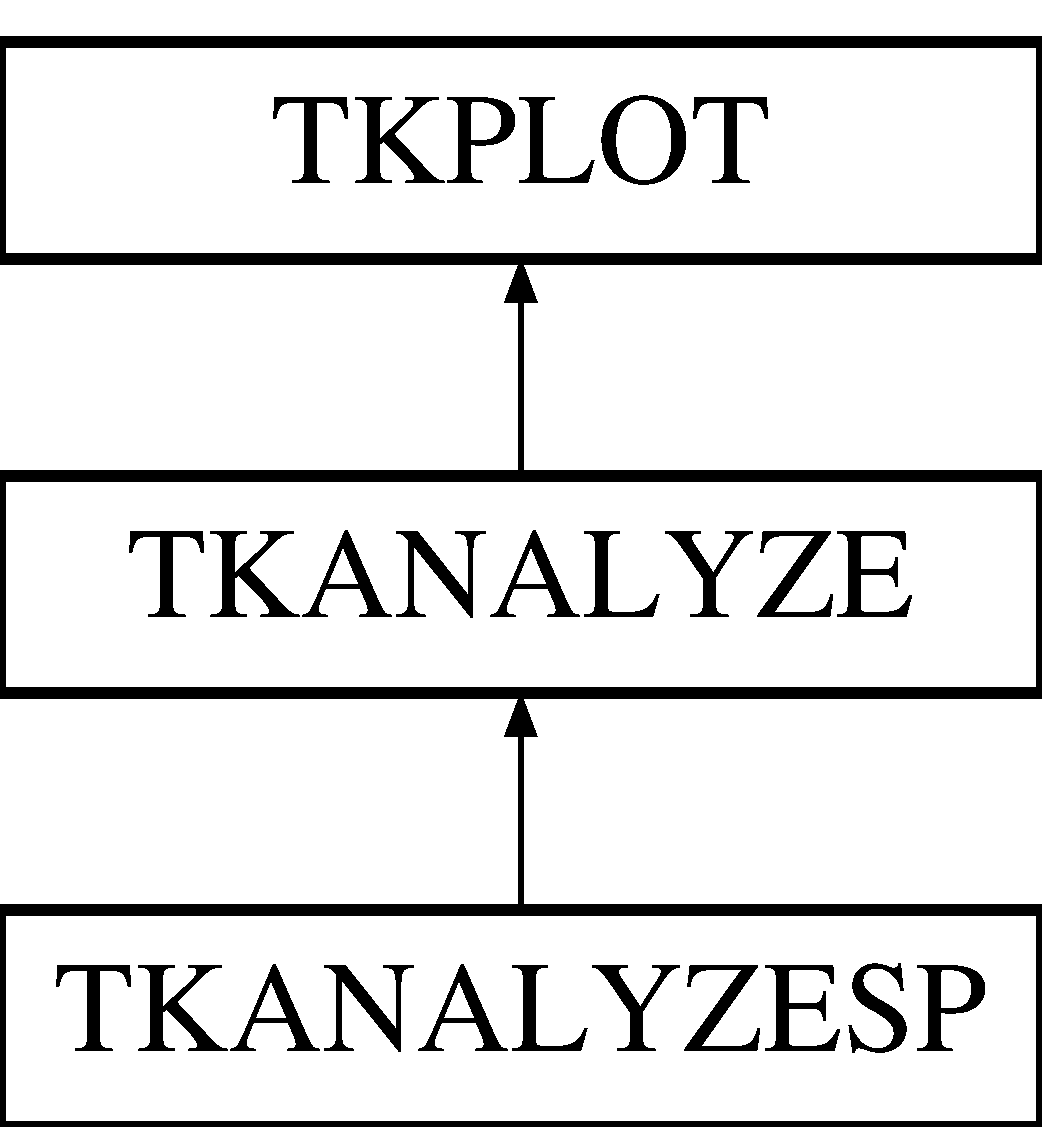
\includegraphics[height=3.000000cm]{class_t_k_a_n_a_l_y_z_e_s_p}
\end{center}
\end{figure}
\subsection*{公開メンバ関数}
\begin{DoxyCompactItemize}
\item 
\mbox{\Hypertarget{class_t_k_a_n_a_l_y_z_e_s_p_aa2acb0801185f8627c598bde433e53de}\label{class_t_k_a_n_a_l_y_z_e_s_p_aa2acb0801185f8627c598bde433e53de}} 
{\bfseries T\+K\+A\+N\+A\+L\+Y\+Z\+E\+SP} (\hyperlink{class_t_k_s_h_o_t}{T\+K\+S\+H\+OT} $\ast$T\+K\+Shot\+\_\+, clx\+::ini $\ast$Setting\+\_\+, std\+::string group\+\_\+)
\item 
\mbox{\Hypertarget{class_t_k_a_n_a_l_y_z_e_s_p_a960444249fc72e7b65c8d7176be04201}\label{class_t_k_a_n_a_l_y_z_e_s_p_a960444249fc72e7b65c8d7176be04201}} 
void {\bfseries Set\+M\+A\+Sample\+Number} (int sample\+\_\+number)
\item 
\mbox{\Hypertarget{class_t_k_a_n_a_l_y_z_e_s_p_a1b8358ffef8bcce3c2855f523247d9bb}\label{class_t_k_a_n_a_l_y_z_e_s_p_a1b8358ffef8bcce3c2855f523247d9bb}} 
int {\bfseries Plot\+Analyze\+SP} (\hyperlink{class_t_k_p_l_o_t_a158082ae168750554cf23edde9a27416}{T\+K\+P\+L\+O\+T\+::\+P\+L\+O\+T\+S\+I\+ZE} plot\+\_\+size, int shot\+\_\+number)
\end{DoxyCompactItemize}
\subsection*{その他の継承メンバ}


このクラス詳解は次のファイルから抽出されました\+:\begin{DoxyCompactItemize}
\item 
tkanalyzesp.\+h\end{DoxyCompactItemize}

\hypertarget{class_t_k_d_a_t_a}{}\section{T\+K\+D\+A\+TA クラス}
\label{class_t_k_d_a_t_a}\index{T\+K\+D\+A\+TA@{T\+K\+D\+A\+TA}}
\subsection*{公開型}
\begin{DoxyCompactItemize}
\item 
\mbox{\Hypertarget{class_t_k_d_a_t_a_ab55f2c2d1c76bbeb3c1820ad2e749f38}\label{class_t_k_d_a_t_a_ab55f2c2d1c76bbeb3c1820ad2e749f38}} 
enum {\bfseries B\+Y\+T\+E\+O\+R\+D\+ER} \{ {\bfseries B\+I\+G\+\_\+\+E\+N\+D\+I\+AN}, 
{\bfseries L\+I\+T\+T\+L\+E\+\_\+\+E\+N\+D\+I\+AN}
 \}
\item 
\mbox{\Hypertarget{class_t_k_d_a_t_a_add3f58dbf65c97f4c9998e3a8b3f79fd}\label{class_t_k_d_a_t_a_add3f58dbf65c97f4c9998e3a8b3f79fd}} 
enum {\bfseries D\+A\+T\+A\+F\+O\+R\+M\+AT} \{ {\bfseries T\+R\+A\+CE}, 
{\bfseries B\+L\+O\+CK}
 \}
\end{DoxyCompactItemize}
\subsection*{公開メンバ関数}
\begin{DoxyCompactItemize}
\item 
\mbox{\Hypertarget{class_t_k_d_a_t_a_ad142911ef868b94bd2607ab4ca69f84d}\label{class_t_k_d_a_t_a_ad142911ef868b94bd2607ab4ca69f84d}} 
int {\bfseries Parse\+H\+DR} ()
\item 
\mbox{\Hypertarget{class_t_k_d_a_t_a_a64f288a761012bf276a5aa7f74dfcb44}\label{class_t_k_d_a_t_a_a64f288a761012bf276a5aa7f74dfcb44}} 
int {\bfseries Set\+A\+D\+C\+ID} (int iadc\+\_\+id)
\item 
\mbox{\Hypertarget{class_t_k_d_a_t_a_ad0a8defdf8de2ef2bbe42d7d8a53e051}\label{class_t_k_d_a_t_a_ad0a8defdf8de2ef2bbe42d7d8a53e051}} 
int {\bfseries Get\+A\+D\+C\+ID} ()
\item 
\mbox{\Hypertarget{class_t_k_d_a_t_a_ae63b673fda97ff6fef659f51fe40dbe8}\label{class_t_k_d_a_t_a_ae63b673fda97ff6fef659f51fe40dbe8}} 
int {\bfseries Set\+Data\+File\+Name} (std\+::string idata\+\_\+file\+\_\+name)
\item 
\mbox{\Hypertarget{class_t_k_d_a_t_a_a3f354a0eb29025867cbd1e3e27f8e41a}\label{class_t_k_d_a_t_a_a3f354a0eb29025867cbd1e3e27f8e41a}} 
std\+::string {\bfseries Get\+Data\+File\+Name} ()
\item 
\mbox{\Hypertarget{class_t_k_d_a_t_a_a0f0c38948586490c1bfe1f820418c5ef}\label{class_t_k_d_a_t_a_a0f0c38948586490c1bfe1f820418c5ef}} 
float {\bfseries Get\+H\+Resolution} ()
\item 
\mbox{\Hypertarget{class_t_k_d_a_t_a_a6c83babefbef168db08ca1c00cfe560d}\label{class_t_k_d_a_t_a_a6c83babefbef168db08ca1c00cfe560d}} 
float {\bfseries Get\+V\+Offset} (int const trace\+\_\+index)
\item 
\mbox{\Hypertarget{class_t_k_d_a_t_a_a78fccdabf4c7326ecb9dbe30ebe765e4}\label{class_t_k_d_a_t_a_a78fccdabf4c7326ecb9dbe30ebe765e4}} 
float {\bfseries Get\+V\+Resolution} (int const trace\+\_\+index)
\item 
\mbox{\Hypertarget{class_t_k_d_a_t_a_aaa91499a0c86542c6d240f07b2c7a5a6}\label{class_t_k_d_a_t_a_aaa91499a0c86542c6d240f07b2c7a5a6}} 
int {\bfseries Get\+V\+Max\+Data} (int const trace\+\_\+index)
\item 
\mbox{\Hypertarget{class_t_k_d_a_t_a_aed38093c0f7a086ab190c89770567531}\label{class_t_k_d_a_t_a_aed38093c0f7a086ab190c89770567531}} 
int {\bfseries Get\+V\+Min\+Data} (int const trace\+\_\+index)
\item 
\mbox{\Hypertarget{class_t_k_d_a_t_a_a5fe237cba051e352845786e13c0cd54f}\label{class_t_k_d_a_t_a_a5fe237cba051e352845786e13c0cd54f}} 
int {\bfseries Get\+Block\+Size} ()
\item 
\mbox{\Hypertarget{class_t_k_d_a_t_a_ac823854fcfb02d7788ec491b38f4d615}\label{class_t_k_d_a_t_a_ac823854fcfb02d7788ec491b38f4d615}} 
float {\bfseries Get\+H\+Offset} ()
\item 
\mbox{\Hypertarget{class_t_k_d_a_t_a_af0a676448ec4d492290517a7e60a2de3}\label{class_t_k_d_a_t_a_af0a676448ec4d492290517a7e60a2de3}} 
std\+::string {\bfseries Get\+Model\+Name} ()
\item 
\mbox{\Hypertarget{class_t_k_d_a_t_a_a63437cd1b2448b0b54ee6ec56da1321e}\label{class_t_k_d_a_t_a_a63437cd1b2448b0b54ee6ec56da1321e}} 
T\+K\+D\+A\+T\+A\+::\+B\+Y\+T\+E\+O\+R\+D\+ER {\bfseries Get\+Byte\+Order} ()
\item 
\mbox{\Hypertarget{class_t_k_d_a_t_a_a86117b4edecbf2e3013973fb016877e2}\label{class_t_k_d_a_t_a_a86117b4edecbf2e3013973fb016877e2}} 
T\+K\+D\+A\+T\+A\+::\+D\+A\+T\+A\+F\+O\+R\+M\+AT {\bfseries Get\+Data\+Format} ()
\item 
\mbox{\Hypertarget{class_t_k_d_a_t_a_a11fad512e15a5b8dd7be2ff786d5fd8e}\label{class_t_k_d_a_t_a_a11fad512e15a5b8dd7be2ff786d5fd8e}} 
int {\bfseries Get\+Data\+Offset} ()
\item 
\mbox{\Hypertarget{class_t_k_d_a_t_a_a0e9270376ed47917048fdd38f2f4a81d}\label{class_t_k_d_a_t_a_a0e9270376ed47917048fdd38f2f4a81d}} 
int {\bfseries Get\+Trace\+Total\+Number} ()
\item 
\mbox{\Hypertarget{class_t_k_d_a_t_a_ad70108b9612759566d7cc90e60f293c5}\label{class_t_k_d_a_t_a_ad70108b9612759566d7cc90e60f293c5}} 
int {\bfseries Channnel\+Number\+To\+Trace\+Number} (int const channel\+\_\+number)
\item 
\mbox{\Hypertarget{class_t_k_d_a_t_a_a8282e57fcee3618dfe533b6771adce96}\label{class_t_k_d_a_t_a_a8282e57fcee3618dfe533b6771adce96}} 
int {\bfseries Get\+Channel\+Number} (int const trace\+\_\+index)
\end{DoxyCompactItemize}


このクラス詳解は次のファイルから抽出されました\+:\begin{DoxyCompactItemize}
\item 
tkshotinfo.\+h\item 
tkshotinfo.\+cpp\end{DoxyCompactItemize}

\hypertarget{class_t_k_particle_palameter}{}\section{T\+K\+Particle\+Palameter クラス}
\label{class_t_k_particle_palameter}\index{T\+K\+Particle\+Palameter@{T\+K\+Particle\+Palameter}}
\subsection*{公開変数類}
\begin{DoxyCompactItemize}
\item 
\mbox{\Hypertarget{class_t_k_particle_palameter_a23ae16244a4143ee0642cf6620facf31}\label{class_t_k_particle_palameter_a23ae16244a4143ee0642cf6620facf31}} 
double {\bfseries density}
\item 
\mbox{\Hypertarget{class_t_k_particle_palameter_a65c396039f6aaf454837c2139af9da65}\label{class_t_k_particle_palameter_a65c396039f6aaf454837c2139af9da65}} 
double {\bfseries temperature}
\item 
\mbox{\Hypertarget{class_t_k_particle_palameter_a9be89d1ba1cb6c97e6154bf9f91f2437}\label{class_t_k_particle_palameter_a9be89d1ba1cb6c97e6154bf9f91f2437}} 
double {\bfseries mass}
\end{DoxyCompactItemize}


このクラス詳解は次のファイルから抽出されました\+:\begin{DoxyCompactItemize}
\item 
U\+I/\+Project1/tkphysics.\+h\end{DoxyCompactItemize}

\hypertarget{class_t_k_plasma}{}\section{T\+K\+Plasma クラス}
\label{class_t_k_plasma}\index{T\+K\+Plasma@{T\+K\+Plasma}}
\subsection*{公開変数類}
\begin{DoxyCompactItemize}
\item 
\mbox{\Hypertarget{class_t_k_plasma_ab2ba31fba9c3b255fa454d557b46c552}\label{class_t_k_plasma_ab2ba31fba9c3b255fa454d557b46c552}} 
double const  \& {\bfseries n\+\_\+e} = electron.\+density
\item 
\mbox{\Hypertarget{class_t_k_plasma_af742f3b64a9c48f6f0e3184bf7ebb0c2}\label{class_t_k_plasma_af742f3b64a9c48f6f0e3184bf7ebb0c2}} 
double const  \& {\bfseries n\+\_\+n} = neutral.\+density
\item 
\mbox{\Hypertarget{class_t_k_plasma_a0074fb0c178f69de84d5509d0bfd4ac0}\label{class_t_k_plasma_a0074fb0c178f69de84d5509d0bfd4ac0}} 
double const {\bfseries a}
\end{DoxyCompactItemize}


このクラス詳解は次のファイルから抽出されました\+:\begin{DoxyCompactItemize}
\item 
U\+I/\+Project1/tkphysics.\+h\end{DoxyCompactItemize}

\hypertarget{class_t_k_plasma_parameter}{}\section{T\+K\+Plasma\+Parameter クラス}
\label{class_t_k_plasma_parameter}\index{T\+K\+Plasma\+Parameter@{T\+K\+Plasma\+Parameter}}


このクラス詳解は次のファイルから抽出されました\+:\begin{DoxyCompactItemize}
\item 
tkphysics.\+h\end{DoxyCompactItemize}

\hypertarget{class_t_k_p_l_o_t}{}\section{T\+K\+P\+L\+OT クラス}
\label{class_t_k_p_l_o_t}\index{T\+K\+P\+L\+OT@{T\+K\+P\+L\+OT}}


{\ttfamily \#include $<$tkplot.\+h$>$}

T\+K\+P\+L\+OT の継承関係図\begin{figure}[H]
\begin{center}
\leavevmode
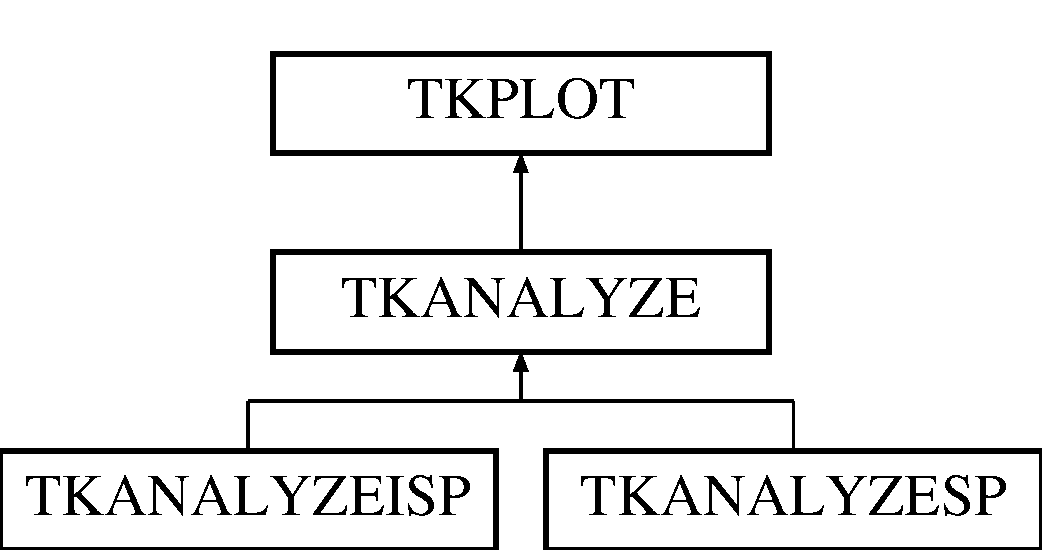
\includegraphics[height=3.000000cm]{class_t_k_p_l_o_t}
\end{center}
\end{figure}
\subsection*{クラス}
\begin{DoxyCompactItemize}
\item 
class \hyperlink{class_t_k_p_l_o_t_1_1_p_l_o_t_i_n_f_o}{P\+L\+O\+T\+I\+N\+FO}
\item 
class \hyperlink{class_t_k_p_l_o_t_1_1_p_o_s_i_t_i_o_n}{P\+O\+S\+I\+T\+I\+ON}
\item 
class \hyperlink{class_t_k_p_l_o_t_1_1_r_a_n_g_e}{R\+A\+N\+GE}
\item 
class \hyperlink{class_t_k_p_l_o_t_1_1_s_i_z_e}{S\+I\+ZE}
\end{DoxyCompactItemize}
\subsection*{公開型}
\begin{DoxyCompactItemize}
\item 
enum \hyperlink{class_t_k_p_l_o_t_a158082ae168750554cf23edde9a27416}{P\+L\+O\+T\+S\+I\+ZE} \{ {\bfseries S\+M\+A\+L\+L\+\_\+\+S\+I\+ZE}, 
{\bfseries M\+E\+D\+I\+U\+M\+\_\+\+S\+I\+ZE}
 \}
\item 
enum \hyperlink{class_t_k_p_l_o_t_a28dfea1dd78dfc49c1926518da615bfa}{D\+A\+T\+A\+S\+O\+U\+R\+CE} \{ \hyperlink{class_t_k_p_l_o_t_a28dfea1dd78dfc49c1926518da615bfaa98ad0e8750ae10ad556ed7a62affb452}{D\+A\+T\+A\+S\+O\+U\+R\+C\+E\+::\+B\+I\+N\+A\+RY}, 
\hyperlink{class_t_k_p_l_o_t_a28dfea1dd78dfc49c1926518da615bfaad2cd8253361a9c732d21ca1d336599cc}{D\+A\+T\+A\+S\+O\+U\+R\+C\+E\+::\+A\+S\+C\+II}
 \}
\end{DoxyCompactItemize}
\subsection*{公開メンバ関数}
\begin{DoxyCompactItemize}
\item 
\mbox{\Hypertarget{class_t_k_p_l_o_t_aeb9168bcf7e45c45fc38dab63e6b90b3}\label{class_t_k_p_l_o_t_aeb9168bcf7e45c45fc38dab63e6b90b3}} 
{\bfseries T\+K\+P\+L\+OT} (\hyperlink{class_t_k_s_h_o_t}{T\+K\+S\+H\+OT} $\ast$T\+K\+Shot\+\_\+)
\item 
\mbox{\Hypertarget{class_t_k_p_l_o_t_a0dcffb0672762042e8dca5791b97e182}\label{class_t_k_p_l_o_t_a0dcffb0672762042e8dca5791b97e182}} 
int {\bfseries Plot\+Raw} (const \hyperlink{class_t_k_p_l_o_t_a158082ae168750554cf23edde9a27416}{T\+K\+P\+L\+O\+T\+::\+P\+L\+O\+T\+S\+I\+ZE} plot\+\_\+size, const int shot\+\_\+number, bool replot=true)
\item 
\mbox{\Hypertarget{class_t_k_p_l_o_t_a5ddc4ef2a68d8649cfb2aebf507121fd}\label{class_t_k_p_l_o_t_a5ddc4ef2a68d8649cfb2aebf507121fd}} 
std\+::vector$<$ \hyperlink{class_t_k_p_l_o_t_1_1_p_l_o_t_i_n_f_o}{T\+K\+P\+L\+O\+T\+::\+P\+L\+O\+T\+I\+N\+FO} $>$ {\bfseries Get\+Plot\+Info} ()
\item 
\mbox{\Hypertarget{class_t_k_p_l_o_t_a4087cc1a73e760ac8eb32cbdf78a4433}\label{class_t_k_p_l_o_t_a4087cc1a73e760ac8eb32cbdf78a4433}} 
std\+::vector$<$ \hyperlink{class_t_k_p_l_o_t_1_1_p_l_o_t_i_n_f_o}{T\+K\+P\+L\+O\+T\+::\+P\+L\+O\+T\+I\+N\+FO} $>$\+::pointer {\bfseries Get\+Plot\+Info\+Ptr} ()
\end{DoxyCompactItemize}
\subsection*{限定公開メンバ関数}
\begin{DoxyCompactItemize}
\item 
\mbox{\Hypertarget{class_t_k_p_l_o_t_aae92c92917093101c52d08d132aee75b}\label{class_t_k_p_l_o_t_aae92c92917093101c52d08d132aee75b}} 
\hyperlink{class_t_k_p_l_o_t_1_1_p_l_o_t_i_n_f_o}{P\+L\+O\+T\+I\+N\+FO} \& {\bfseries load\+Plot\+Info\+Instance} (const int data\+\_\+index, const int trace\+\_\+index, const \hyperlink{class_t_k_p_l_o_t_a158082ae168750554cf23edde9a27416}{P\+L\+O\+T\+S\+I\+ZE} plot\+\_\+size=P\+L\+O\+T\+S\+I\+Z\+E\+::\+S\+M\+A\+L\+L\+\_\+\+S\+I\+ZE)
\end{DoxyCompactItemize}


\subsection{詳解}
グラフ描画に関するクラスです。 

\subsection{列挙型メンバ詳解}
\mbox{\Hypertarget{class_t_k_p_l_o_t_a28dfea1dd78dfc49c1926518da615bfa}\label{class_t_k_p_l_o_t_a28dfea1dd78dfc49c1926518da615bfa}} 
\index{T\+K\+P\+L\+OT@{T\+K\+P\+L\+OT}!D\+A\+T\+A\+S\+O\+U\+R\+CE@{D\+A\+T\+A\+S\+O\+U\+R\+CE}}
\index{D\+A\+T\+A\+S\+O\+U\+R\+CE@{D\+A\+T\+A\+S\+O\+U\+R\+CE}!T\+K\+P\+L\+OT@{T\+K\+P\+L\+OT}}
\subsubsection{\texorpdfstring{D\+A\+T\+A\+S\+O\+U\+R\+CE}{DATASOURCE}}
{\footnotesize\ttfamily enum \hyperlink{class_t_k_p_l_o_t_a28dfea1dd78dfc49c1926518da615bfa}{T\+K\+P\+L\+O\+T\+::\+D\+A\+T\+A\+S\+O\+U\+R\+CE}\hspace{0.3cm}{\ttfamily [strong]}}

データファイル形式型 \begin{DoxyEnumFields}{列挙値}
\raisebox{\heightof{T}}[0pt][0pt]{\index{B\+I\+N\+A\+RY@{B\+I\+N\+A\+RY}!T\+K\+P\+L\+OT@{T\+K\+P\+L\+OT}}\index{T\+K\+P\+L\+OT@{T\+K\+P\+L\+OT}!B\+I\+N\+A\+RY@{B\+I\+N\+A\+RY}}}\mbox{\Hypertarget{class_t_k_p_l_o_t_a28dfea1dd78dfc49c1926518da615bfaa98ad0e8750ae10ad556ed7a62affb452}\label{class_t_k_p_l_o_t_a28dfea1dd78dfc49c1926518da615bfaa98ad0e8750ae10ad556ed7a62affb452}} 
B\+I\+N\+A\+RY&バイナリファイル~\newline
 非常に高速に処理できますが、柔軟性にかけるため使用できないことがあります。 \\
\hline

\raisebox{\heightof{T}}[0pt][0pt]{\index{A\+S\+C\+II@{A\+S\+C\+II}!T\+K\+P\+L\+OT@{T\+K\+P\+L\+OT}}\index{T\+K\+P\+L\+OT@{T\+K\+P\+L\+OT}!A\+S\+C\+II@{A\+S\+C\+II}}}\mbox{\Hypertarget{class_t_k_p_l_o_t_a28dfea1dd78dfc49c1926518da615bfaad2cd8253361a9c732d21ca1d336599cc}\label{class_t_k_p_l_o_t_a28dfea1dd78dfc49c1926518da615bfaad2cd8253361a9c732d21ca1d336599cc}} 
A\+S\+C\+II&A\+S\+C\+I\+Iファイル~\newline
 データ変換のイニシャルタイムが必要であり、データ読み込みもハイコストなため、処理は遅くなりますが、全ての機能を利用できます。 \\
\hline

\end{DoxyEnumFields}
\mbox{\Hypertarget{class_t_k_p_l_o_t_a158082ae168750554cf23edde9a27416}\label{class_t_k_p_l_o_t_a158082ae168750554cf23edde9a27416}} 
\index{T\+K\+P\+L\+OT@{T\+K\+P\+L\+OT}!P\+L\+O\+T\+S\+I\+ZE@{P\+L\+O\+T\+S\+I\+ZE}}
\index{P\+L\+O\+T\+S\+I\+ZE@{P\+L\+O\+T\+S\+I\+ZE}!T\+K\+P\+L\+OT@{T\+K\+P\+L\+OT}}
\subsubsection{\texorpdfstring{P\+L\+O\+T\+S\+I\+ZE}{PLOTSIZE}}
{\footnotesize\ttfamily enum \hyperlink{class_t_k_p_l_o_t_a158082ae168750554cf23edde9a27416}{T\+K\+P\+L\+O\+T\+::\+P\+L\+O\+T\+S\+I\+ZE}\hspace{0.3cm}{\ttfamily [strong]}}

グラフサイズ型 

このクラス詳解は次のファイルから抽出されました\+:\begin{DoxyCompactItemize}
\item 
tkplot.\+h\end{DoxyCompactItemize}

\hypertarget{class_t_k_s_h_o_t}{}\section{T\+K\+S\+H\+OT クラス}
\label{class_t_k_s_h_o_t}\index{T\+K\+S\+H\+OT@{T\+K\+S\+H\+OT}}
\subsection*{公開メンバ関数}
\begin{DoxyCompactItemize}
\item 
\mbox{\Hypertarget{class_t_k_s_h_o_t_af116d5e195d9853c78d3e4ddb00e2c57}\label{class_t_k_s_h_o_t_af116d5e195d9853c78d3e4ddb00e2c57}} 
int {\bfseries Get\+A\+D\+C\+Number} ()
\item 
\mbox{\Hypertarget{class_t_k_s_h_o_t_ac102eb99258f9950569960d73f9ce946}\label{class_t_k_s_h_o_t_ac102eb99258f9950569960d73f9ce946}} 
std\+::string {\bfseries Get\+Data\+File\+Name} (T\+K\+A\+D\+C\+I\+N\+F\+O\+::\+A\+D\+C\+ID adc\+\_\+id)
\item 
\mbox{\Hypertarget{class_t_k_s_h_o_t_a8f91dff3640a574152c6fb3c5e542f62}\label{class_t_k_s_h_o_t_a8f91dff3640a574152c6fb3c5e542f62}} 
int {\bfseries Name\+Shot\+Number} (int ishot\+\_\+number)
\item 
\mbox{\Hypertarget{class_t_k_s_h_o_t_a8edc2c710c0dd04d619ddb5f105c41fe}\label{class_t_k_s_h_o_t_a8edc2c710c0dd04d619ddb5f105c41fe}} 
int {\bfseries Clear} ()
\item 
\mbox{\Hypertarget{class_t_k_s_h_o_t_a6337475c0a3915a1c9ecdea289c30258}\label{class_t_k_s_h_o_t_a6337475c0a3915a1c9ecdea289c30258}} 
int {\bfseries Append\+Data\+File} (T\+K\+A\+D\+C\+I\+N\+F\+O\+::\+A\+D\+C\+ID adc\+\_\+id, std\+::string data\+\_\+file\+\_\+name)
\item 
\mbox{\Hypertarget{class_t_k_s_h_o_t_a1d6b251b7f6606df57fcd727ea062433}\label{class_t_k_s_h_o_t_a1d6b251b7f6606df57fcd727ea062433}} 
float {\bfseries Get\+H\+Resolution} (T\+K\+A\+D\+C\+I\+N\+F\+O\+::\+A\+D\+C\+ID adc\+\_\+id)
\item 
\mbox{\Hypertarget{class_t_k_s_h_o_t_a5edbf2e53db13a8577fea4d8e9c7757b}\label{class_t_k_s_h_o_t_a5edbf2e53db13a8577fea4d8e9c7757b}} 
int {\bfseries Get\+Block\+Size} (T\+K\+A\+D\+C\+I\+N\+F\+O\+::\+A\+D\+C\+ID adc\+\_\+id)
\item 
\mbox{\Hypertarget{class_t_k_s_h_o_t_a94ad848c94a6328f12fa77af5be167f9}\label{class_t_k_s_h_o_t_a94ad848c94a6328f12fa77af5be167f9}} 
float {\bfseries Get\+V\+Offset} (T\+K\+A\+D\+C\+I\+N\+F\+O\+::\+A\+D\+C\+ID adc\+\_\+id, int trace\+\_\+index)
\item 
\mbox{\Hypertarget{class_t_k_s_h_o_t_a46eb57e1564b7f64647c4a7450219780}\label{class_t_k_s_h_o_t_a46eb57e1564b7f64647c4a7450219780}} 
float {\bfseries Get\+V\+Resolution} (T\+K\+A\+D\+C\+I\+N\+F\+O\+::\+A\+D\+C\+ID adc\+\_\+id, int trace\+\_\+index)
\item 
\mbox{\Hypertarget{class_t_k_s_h_o_t_ad6d95c6c53f8b406e24fd05daa9a96b0}\label{class_t_k_s_h_o_t_ad6d95c6c53f8b406e24fd05daa9a96b0}} 
int {\bfseries Get\+V\+Max\+Data} (T\+K\+A\+D\+C\+I\+N\+F\+O\+::\+A\+D\+C\+ID adc\+\_\+id, int trace\+\_\+index)
\item 
\mbox{\Hypertarget{class_t_k_s_h_o_t_a65e951c7890ee7b9bef635beb54070cf}\label{class_t_k_s_h_o_t_a65e951c7890ee7b9bef635beb54070cf}} 
int {\bfseries Get\+V\+Min\+Data} (T\+K\+A\+D\+C\+I\+N\+F\+O\+::\+A\+D\+C\+ID adc\+\_\+id, int trace\+\_\+index)
\item 
\mbox{\Hypertarget{class_t_k_s_h_o_t_ae502263f7b666c4c7d1e5f044a89924f}\label{class_t_k_s_h_o_t_ae502263f7b666c4c7d1e5f044a89924f}} 
float {\bfseries Get\+H\+Offset} (T\+K\+A\+D\+C\+I\+N\+F\+O\+::\+A\+D\+C\+ID adc\+\_\+id)
\item 
\mbox{\Hypertarget{class_t_k_s_h_o_t_a11a6d38c2cd9a720e5df9c7b482f479d}\label{class_t_k_s_h_o_t_a11a6d38c2cd9a720e5df9c7b482f479d}} 
std\+::string {\bfseries Get\+Model\+Name} (T\+K\+A\+D\+C\+I\+N\+F\+O\+::\+A\+D\+C\+ID adc\+\_\+id)
\item 
\mbox{\Hypertarget{class_t_k_s_h_o_t_a283bdf8a375795d36e9a985dd2920bfa}\label{class_t_k_s_h_o_t_a283bdf8a375795d36e9a985dd2920bfa}} 
int {\bfseries Get\+Trace\+Total\+Number} (T\+K\+A\+D\+C\+I\+N\+F\+O\+::\+A\+D\+C\+ID adc\+\_\+id)
\item 
\mbox{\Hypertarget{class_t_k_s_h_o_t_a9bc227a4b7645835e479fcbded5943bd}\label{class_t_k_s_h_o_t_a9bc227a4b7645835e479fcbded5943bd}} 
int {\bfseries A\+D\+C\+I\+D\+To\+A\+D\+C\+Data\+Index} (T\+K\+A\+D\+C\+I\+N\+F\+O\+::\+A\+D\+C\+ID adc\+\_\+id)
\item 
\mbox{\Hypertarget{class_t_k_s_h_o_t_a4194894bebb1794a6e5a89817f0deaf0}\label{class_t_k_s_h_o_t_a4194894bebb1794a6e5a89817f0deaf0}} 
T\+K\+A\+D\+C\+I\+N\+F\+O\+::\+A\+D\+C\+ID {\bfseries Get\+A\+D\+C\+ID} (int adc\+\_\+index)
\item 
\mbox{\Hypertarget{class_t_k_s_h_o_t_ac7be926f62c580023119be4cb23fb4d2}\label{class_t_k_s_h_o_t_ac7be926f62c580023119be4cb23fb4d2}} 
int {\bfseries Get\+Channel\+Number} (T\+K\+A\+D\+C\+I\+N\+F\+O\+::\+A\+D\+C\+ID adc\+\_\+id, int trace\+\_\+index)
\end{DoxyCompactItemize}


このクラス詳解は次のファイルから抽出されました\+:\begin{DoxyCompactItemize}
\item 
tkshotinfo.\+h\end{DoxyCompactItemize}

\hypertarget{struct_project1_1_1_my_form_1_1clx_1_1detail_1_1widest__char}{}\section{Project1\+:\+:My\+Form\+:\+:clx\+:\+:detail\+:\+:widest\+\_\+char$<$ Type\+Char, Source\+Char $>$ 構造体テンプレート}
\label{struct_project1_1_1_my_form_1_1clx_1_1detail_1_1widest__char}\index{Project1\+::\+My\+Form\+::clx\+::detail\+::widest\+\_\+char$<$ Type\+Char, Source\+Char $>$@{Project1\+::\+My\+Form\+::clx\+::detail\+::widest\+\_\+char$<$ Type\+Char, Source\+Char $>$}}
\subsection*{公開型}
\begin{DoxyCompactItemize}
\item 
\mbox{\Hypertarget{struct_project1_1_1_my_form_1_1clx_1_1detail_1_1widest__char_a4aa71a0d7a47cc56ba9b8520126f8b21}\label{struct_project1_1_1_my_form_1_1clx_1_1detail_1_1widest__char_a4aa71a0d7a47cc56ba9b8520126f8b21}} 
typedef Type\+Char {\bfseries type}
\end{DoxyCompactItemize}


この構造体詳解は次のファイルから抽出されました\+:\begin{DoxyCompactItemize}
\item 
My\+Form.\+h\end{DoxyCompactItemize}

\chapter{ファイル詳解}
\hypertarget{tkadc_8h}{}\section{tkadc.\+h ファイル}
\label{tkadc_8h}\index{tkadc.\+h@{tkadc.\+h}}


A\+D\+Cをコントロールするためのクラスを宣言しています。 A\+D\+Cの制御に関して、モデルに依存する部分はここに記述してください。  


{\ttfamily \#include $<$string$>$}\newline
{\ttfamily \#include $<$iostream$>$}\newline
{\ttfamily \#include \char`\"{}tmctl.\+h\char`\"{}}\newline
\subsection*{クラス}
\begin{DoxyCompactItemize}
\item 
class \hyperlink{class_t_k_a_d_c_c_o_n_t_r_o_l}{T\+K\+A\+D\+C\+C\+O\+N\+T\+R\+OL}
\item 
class \hyperlink{class_t_k_a_d_c_c_o_n_t_r_o_l_1_1_exception}{T\+K\+A\+D\+C\+C\+O\+N\+T\+R\+O\+L\+::\+Exception}
\item 
class \hyperlink{class_t_k_a_d_c_c_o_n_t_r_o_l___d_l750}{T\+K\+A\+D\+C\+C\+O\+N\+T\+R\+O\+L\+\_\+\+D\+L750}
\item 
class \hyperlink{class_t_k_a_d_c_c_o_n_t_r_o_l___d_l850}{T\+K\+A\+D\+C\+C\+O\+N\+T\+R\+O\+L\+\_\+\+D\+L850}
\end{DoxyCompactItemize}
\subsection*{マクロ定義}
\begin{DoxyCompactItemize}
\item 
\mbox{\Hypertarget{tkadc_8h_adc3098545276669ab4c4771eb395bbc2}\label{tkadc_8h_adc3098545276669ab4c4771eb395bbc2}} 
\#define {\bfseries T\+K\+A\+D\+C\+\_\+\+A\+D\+C\+\_\+\+M\+O\+D\+E\+L\+\_\+\+D\+L750}~T\+K\+A\+D\+C\+C\+O\+N\+T\+R\+O\+L\+::\+A\+D\+C\+M\+O\+D\+E\+L\+::\+D\+L750
\item 
\mbox{\Hypertarget{tkadc_8h_a97e18823dd95e64bea5292f9d23ea048}\label{tkadc_8h_a97e18823dd95e64bea5292f9d23ea048}} 
\#define {\bfseries T\+K\+A\+D\+C\+\_\+\+A\+D\+C\+\_\+\+M\+O\+D\+E\+L\+\_\+\+D\+L850}~T\+K\+A\+D\+C\+C\+O\+N\+T\+R\+O\+L\+::\+A\+D\+C\+M\+O\+D\+E\+L\+::\+D\+L850
\item 
\mbox{\Hypertarget{tkadc_8h_a881027a2354a0e19afa983c2dc4b3e11}\label{tkadc_8h_a881027a2354a0e19afa983c2dc4b3e11}} 
\#define {\bfseries T\+K\+A\+D\+C\+\_\+\+A\+D\+C\+\_\+\+C\+H\+A\+N\+N\+E\+L\+\_\+\+M\+AX}~18
\end{DoxyCompactItemize}


\subsection{詳解}
A\+D\+Cをコントロールするためのクラスを宣言しています。 A\+D\+Cの制御に関して、モデルに依存する部分はここに記述してください。 

\begin{DoxyAuthor}{著者}
Kobayashi Takahiko 
\end{DoxyAuthor}
\begin{DoxyDate}{日付}
2017 
\end{DoxyDate}

\hypertarget{tkutil_8h}{}\section{U\+I/\+Project1/tkutil.h ファイル}
\label{tkutil_8h}\index{U\+I/\+Project1/tkutil.\+h@{U\+I/\+Project1/tkutil.\+h}}


�֗��Ȕėp�֐����ł��B  


{\ttfamily \#include $<$iostream$>$}\newline
{\ttfamily \#include $<$string$>$}\newline
{\ttfamily \#include $<$sstream$>$}\newline
{\ttfamily \#include $<$iomanip$>$}\newline
{\ttfamily \#include $<$fstream$>$}\newline
\subsection*{関数}
\begin{DoxyCompactItemize}
\item 
std\+::string \hyperlink{tkutil_8h_a02b37f2f23e258b7a44b83e1ac5b81b7}{T\+K\+U\+T\+I\+L\+::\+Zero\+Fill} (int const number, int const length)
\item 
bool \hyperlink{tkutil_8h_ab26eef58ef280f33492f52cb4fbe6b5d}{T\+K\+U\+T\+I\+L\+::\+Is\+Exist\+File} (std\+::string const file\+\_\+name)
\end{DoxyCompactItemize}


\subsection{詳解}
�֗��Ȕėp�֐����ł��B 

\begin{DoxyAuthor}{著者}
Kobayashi Takahiko 
\end{DoxyAuthor}
\begin{DoxyDate}{日付}
2017 
\end{DoxyDate}


\subsection{関数詳解}
\mbox{\Hypertarget{tkutil_8h_file_ab26eef58ef280f33492f52cb4fbe6b5d}\label{tkutil_8h_file_ab26eef58ef280f33492f52cb4fbe6b5d}} 
\index{tkutil.\+h@{tkutil.\+h}!Is\+Exist\+File@{Is\+Exist\+File}}
\index{Is\+Exist\+File@{Is\+Exist\+File}!tkutil.\+h@{tkutil.\+h}}
\subsubsection{\texorpdfstring{Is\+Exist\+File()}{IsExistFile()}}
{\footnotesize\ttfamily bool T\+K\+U\+T\+I\+L\+::\+Is\+Exist\+File (\begin{DoxyParamCaption}\item[{std\+::string const}]{file\+\_\+name }\end{DoxyParamCaption})}

�w�肵���t�@�\+C�������݂��邩�ǂ������m���߂܂��B 
\begin{DoxyParams}[1]{引数}
\mbox{\tt in}  & {\em file\+\_\+name} & ���݂��m�\+F����t�@�\+C�����ł��B \\
\hline
\end{DoxyParams}
\begin{DoxyReturn}{戻り値}
true\+: �t�@�\+C���͑��݂��܂��B 

false\+: �t�@�\+C���͑��݂��܂���B 
\end{DoxyReturn}
\begin{DoxyNote}{覚え書き}
�\+J�����Ƃ̂ł��Ȃ��t�@�\+C���͑��݂��Ȃ��Ƃ݂Ȃ���܂��B 
\end{DoxyNote}
\mbox{\Hypertarget{tkutil_8h_file_a02b37f2f23e258b7a44b83e1ac5b81b7}\label{tkutil_8h_file_a02b37f2f23e258b7a44b83e1ac5b81b7}} 
\index{tkutil.\+h@{tkutil.\+h}!Zero\+Fill@{Zero\+Fill}}
\index{Zero\+Fill@{Zero\+Fill}!tkutil.\+h@{tkutil.\+h}}
\subsubsection{\texorpdfstring{Zero\+Fill()}{ZeroFill()}}
{\footnotesize\ttfamily std\+::string T\+K\+U\+T\+I\+L\+::\+Zero\+Fill (\begin{DoxyParamCaption}\item[{int const}]{number,  }\item[{int const}]{length }\end{DoxyParamCaption})}

������\+C�ӌ�����0�Ŗ��߂�������𐶐����܂��B 
\begin{DoxyParams}[1]{引数}
\mbox{\tt in}  & {\em number} & �ΏۂƂȂ鐮���ł��B \\
\hline
\mbox{\tt in}  & {\em length} & �ŏ\+I�\+I�Ȍ����ł��B \\
\hline
\end{DoxyParams}
\begin{DoxyReturn}{戻り値}
�������ꂽstd\+::string�$^\wedge$�̕����񂪕Ԃ���܂��B 
\end{DoxyReturn}

%--- End generated contents ---

% Index
\backmatter
\newpage
\phantomsection
\clearemptydoublepage
\addcontentsline{toc}{chapter}{索引}
\printindex

\end{document}
